\documentclass[12pt,a4paper,hyperref]{ctexrep}
\usepackage{amsmath,amsfonts,amscd,amsthm,dsfont,amssymb,extarrows,mathtools}
\usepackage{color}                           
\usepackage[dvipsnames, svgnames, x11names]{xcolor}
\usepackage{physics}
\usepackage{subfigure}
\usepackage{amsmath}
\usepackage{tikz}
\usepackage{mathdots}
\usepackage{yhmath}
\usepackage{cancel}
\usepackage{color}
\usepackage{siunitx}
\usepackage{array}
\usepackage{multirow}
\usepackage{amssymb}
\usepackage{gensymb}
\usepackage{tabularx}
\usepackage{extarrows}
\usepackage{booktabs}
\usepackage[percent]{overpic}
\usepackage{float}
\usetikzlibrary{fadings}
\usetikzlibrary{patterns}
\usetikzlibrary{shadows.blur}
\usetikzlibrary{shapes}
\usetikzlibrary{arrows}
\usepgflibrary{decorations.markings}
\usetikzlibrary{decorations.markings}

\usetikzlibrary{decorations.pathreplacing}
\usetikzlibrary{shapes,arrows}
\usepackage{footmisc}

\tikzset{
  % style to apply some styles to each segment of a path
  on each segment/.style={
    decorate,
    decoration={
      show path construction,
      moveto code={},
      lineto code={
        \path [#1]
        (\tikzinputsegmentfirst) -- (\tikzinputsegmentlast);
      },
      curveto code={
        \path [#1] (\tikzinputsegmentfirst)
        .. controls
        (\tikzinputsegmentsupporta) and (\tikzinputsegmentsupportb)
        ..
        (\tikzinputsegmentlast);
      },
      closepath code={
        \path [#1]
        (\tikzinputsegmentfirst) -- (\tikzinputsegmentlast);
      },
    },
  },
  % style to add an arrow in the middle of a path
  mid arrow/.style={postaction={decorate,decoration={
        markings,
        mark=at position .5 with {\arrow[#1]{stealth}}
      }}},
}

\newcommand{\dbar}{\overline{\partial}}
\newcommand{\striu}[2][1]{\begin{psmallmatrix} #1 & #2 \\ 0 & #1 \end{psmallmatrix}}
\newcommand{\stril}[2][1]{\begin{psmallmatrix} #1 & 0 \\ #2 & #1 \end{psmallmatrix}}






\begin{document}
\begin{figure}
   \centerline{
   \begin{tikzpicture}[scale=0.8]
                  %\path [fill=pink] (-5,4)--(-5,0) to (-9,0) -- (-9,4);
                  %\path [fill=pink] (-5,-4)--(-5,0) to (-1,0) -- (-1,-4);
      \draw[->][thick](-8,0)--(8,0)node[right]{$Rez$};
      \draw[fill] (0,0) circle [radius=0.05];
      \draw[fill] (-0.4,0)node[below]{$0$} ;
                  %\draw[fill] (4,0)circle [radius=0.05];
                  %\draw[fill] (4.2,0)node[below]{$\xi_{0}$};
                  %\draw[fill] (5.5,0)node[below]{$\xi_{0}+\rho$};
                  %\draw[fill] (2.5,0)node[below]{$\xi_{0}-\rho$};
                  %\draw[-][dashed](3.5,5)--(3.5,-5);
                  %\draw[-][dashed](4.5,5)--(4.5,-5);
      \draw[->][dashed](0,-6)--(0,6);
      \draw[fill] (0,5.5) circle [radius=0.05];
      \draw[fill] (0.2,5.5)node[right]{$\frac{i}{2}$};
      \draw[fill] (0,2) circle [radius=0.05];
      \draw[fill] (-0.2,2)node[left]{$i\kappa_0$};
      \draw[fill] (0,-5.5) circle [radius=0.05];
      \draw[fill] (0.2,-5.5)node[right]{$-\frac{i}{2}$};
      \draw[fill] (0,-2) circle [radius=0.05];
      \draw[fill] (-0.2,-2)node[left]{$-i\kappa_0$};
      \draw[fill] (0,4.8) circle [radius=0.05]node[left]{$z_{j_0}$};
      \draw(0,4.1) [blue, line width=0.5] circle(0.3);
      \draw[fill] (0.3,4.1)node[right]{$z_{j_1}$};
      \draw(0,2.5) [blue, line width=0.5] circle(0.3);
      \draw[fill] (0.3,2.5)node[right]{$z_{j_2}$};
      \draw(0,1) [blue, line width=0.5] circle(0.3);
      \draw[fill] (0.3,1)node[right]{$z_{j_3}$};
      \draw[fill] (0,-5) circle [radius=0.05]node[left]{$\bar{z}_{j_0}$};
      \draw(0,-4.1) [blue, line width=0.5] circle(0.3);
      \draw[fill] (0.3,-4.1)node[right]{$\bar{z}_{j_1}$};
      \draw(0,-2.5) [blue, line width=0.5] circle(0.3);
      \draw[fill] (0.3,-2.5)node[right]{$\bar{z}_{j_2}$};
      \draw(0,-1) [blue, line width=0.5] circle(0.3);
      \draw[fill] (0.3,-1)node[right]{$\bar{z}_{j_3}$};
   \end{tikzpicture}
   }
   \caption{caption}\label{Fig-V-1}
\end{figure}



\clearpage



\begin{figure}
   \centering
   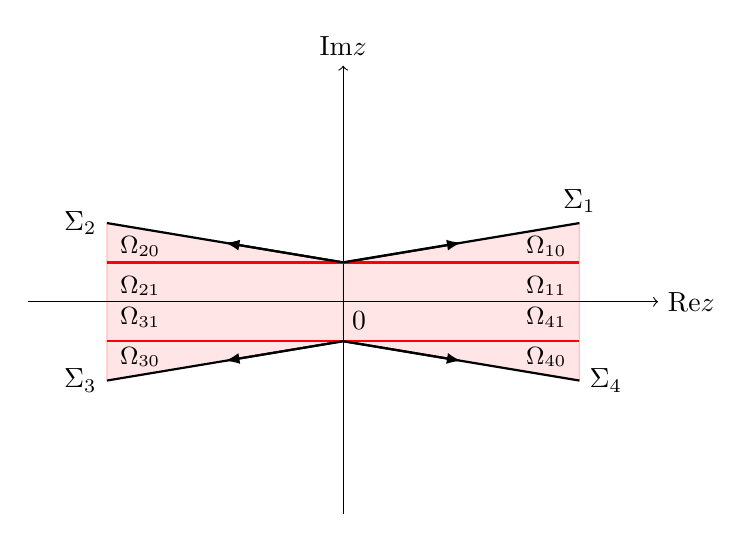
\begin{tikzpicture}[node distance=5cm]
      \draw[pink, fill=pink!40] (0,-0.5)--(3,-1)--(3,1)--(0,0.5)--(0,-0.5)--(-3,-1)--(-3,1)--(0,0.5);
      \draw[thick](0,0.5)--(3,1)node[above]{$\Sigma_1$};
      \draw[thick](0,0.5)--(-3,1)node[left]{$\Sigma_2$};
      \draw[thick](0,-0.5)--(-3,-1)node[left]{$\Sigma_3$};
      \draw[thick](0,-0.5)--(3,-1)node[right]{$\Sigma_4$};
      \draw[->](-4,0)--(4,0)node[right]{ Re$z$};
      \draw[->](0,-2.7)--(0,3)node[above]{ Im$z$};
      \draw[-][thick,red](-3,0.5)--(3,0.5);
      \draw[-][thick,red](-3,-0.5)--(3,-0.5);
      \draw[-latex][thick](0,-0.5)--(-1.5,-0.75);
      \draw[-latex][thick](0,0.5)--(-1.5,0.75);
      \draw[-latex][thick](0,0.5)--(1.5,0.75);
      \draw[-latex][thick](0,-0.5)--(1.5,-0.75);
      \coordinate (I) at (0.2,0);
      \coordinate (C) at (-0.2,2.2);
      \coordinate (D) at (2.2,0.2);
      \fill (D) circle (0pt) node[right] {\small$\Omega_{11}$};
      \coordinate (J) at (-2.2,-0.2);
      \fill (J) circle (0pt) node[left] {\small$\Omega_{31}$};
      \coordinate (k) at (-2.2,0.2);
      \fill (k) circle (0pt) node[left] {\small$\Omega_{21}$};
      \coordinate (k) at (2.2,-0.2);
      \fill (k) circle (0pt) node[right] {\small$\Omega_{41}$};
      \fill (I) circle (0pt) node[below] {$0$};
      \coordinate (a) at (2.2,0.7);
      \fill (a) circle (0pt) node[right] {\small$\Omega_{10}$};
                  %\coordinate (b) at (0.2,2);
                  %     \fill (b) circle (0pt) node[right] {\small$\Omega_{2}$};
      \coordinate (c) at (-2.2,0.7);
      \fill (c) circle (0pt) node[left] {\small$\Omega_{20}$};
      \coordinate (d) at (-2.2,-0.7);
      \fill (d) circle (0pt) node[left] {\small$\Omega_{30}$};
                  %\coordinate (e) at (-0.2,-2);
                  %     \fill (e) circle (0pt) node[left] {\small$\Omega_{5}$};
      \coordinate (f) at (2.2,-0.7);
      \fill (f) circle (0pt) node[right] {\small$\Omega_{40}$};
                  %\coordinate (A) at (2,2.6);
                  %     \coordinate (B) at (2,-2.6);
                  %     \coordinate (C) at (-0.616996232,1.4);
                  %     \coordinate (D) at (-0.616996232,-1.4);
                  %     \coordinate (E) at (1.4,1);
                  %     \coordinate (F) at (1.4,-1);
                  %     \coordinate (G) at (-1.8,2);
                  %     \coordinate (H) at (-1.8,-2);
                  %  \fill (A) circle (1pt) node[right] {$z_1$};
                  %  \fill (B) circle (1pt) node[right] {$\bar{z}_1$};
                  %  \fill (C) circle (1pt) node[left] {$z_2$};
                  %  \fill (D) circle (1pt) node[left] {$\bar{z}_2$};
                  %  \fill (E) circle (1pt) node[right] {$z_3$};
                  %  \fill (F) circle (1pt) node[right] {$\bar{z}_3$};
                  %  \fill (G) circle (1pt) node[left] {$z_4$};
                  %  \fill (H) circle (1pt) node[left] {$\bar{z}_4$};
   \end{tikzpicture}
   \caption{caption}\label{Fig-2}
\end{figure}



\clearpage



\begin{figure}
   \subfigure[]{
   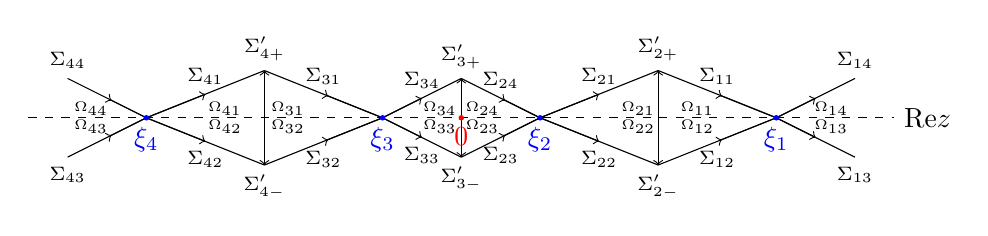
\begin{tikzpicture}
      \draw(-4,0)--(-5,0.5)node[above]{\scriptsize$\Sigma_{44}$};
      \draw[-<](-4,0)--(-4.5,0.25);
      \draw(-4,0)--(-2.5,0.6);
      \draw[->](-4,0)--(-3.25,-0.3)node[below]{\scriptsize$\Sigma_{42}$};
      \draw(-4,0)--(-5,-0.5)node[below]{\scriptsize$\Sigma_{43}$};
      \draw[->](-4,0)--(-3.25,0.3)node[above]{\scriptsize$\Sigma_{41}$};
      \draw(-4,0)--(-2.5,-0.6);
      \draw[-<](-4,0)--(-4.5,-0.25);
      \draw(-1,0)--(0,0.5);
      \draw[->](-1,0)--(-0.5,0.25)node[above]{\scriptsize$\Sigma_{34}$};
      \draw(-1,0)--(-2.5,0.6);
      \draw[-<](-1,0)--(-1.75,-0.3)node[below]{\scriptsize$\Sigma_{32}$};
      \draw(-1,0)--(0,-0.5);
      \draw[-<](-1,0)--(-1.75,0.3)node[above]{\scriptsize$\Sigma_{31}$};
      \draw(-1,0)--(-2.5,-0.6);
      \draw[->](-1,0)--(-0.5,-0.25)node[below]{\scriptsize$\Sigma_{33}$};
      \draw[dashed](-5.5,0)--(5.5,0)node[right]{ Re$z$};
      \draw(1,0)--(0,0.5);
      \draw[-<](1,0)--(0.5,0.25)node[above]{\scriptsize$\Sigma_{24}$};
      \draw(1,0)--(2.5,0.6);
      \draw[->](1,0)--(1.75,-0.3)node[below]{\scriptsize$\Sigma_{22}$};
      \draw(1,0)--(0,-0.5);
      \draw[->](1,0)--(1.75,0.3)node[above]{\scriptsize$\Sigma_{21}$};
      \draw(1,0)--(2.5,-0.6);
      \draw[-<](1,0)--(0.5,-0.25)node[below]{\scriptsize$\Sigma_{23}$};
      \draw(4,0)--(5,0.5)node[above]{\scriptsize$\Sigma_{14}$};
      \draw[->](4,0)--(4.5,0.25);
      \draw(4,0)--(2.5,0.6);
      \draw[-<](4,0)--(3.25,-0.3)node[below]{\scriptsize$\Sigma_{12}$};
      \draw(4,0)--(5,-0.5)node[below]{\scriptsize$\Sigma_{13}$};
      \draw[-<](4,0)--(3.25,0.3)node[above]{\scriptsize$\Sigma_{11}$};
      \draw(4,0)--(2.5,-0.6);
      \draw[->](4,0)--(4.5,-0.25);
      \draw[->](2.5,0)--(2.5,0.6)node[above]{\scriptsize$\Sigma_{2+}'$};
      \draw[->](2.5,0)--(2.5,-0.6)node[below]{\scriptsize$\Sigma_{2-}'$};
      \draw[->](-2.5,0)--(-2.5,0.6)node[above]{\scriptsize$\Sigma_{4+}'$};
      \draw[->](-2.5,0)--(-2.5,-0.6)node[below]{\scriptsize$\Sigma_{4-}'$};
      \draw[->](0,0)--(0,0.5)node[above]{\scriptsize$\Sigma_{3+}'$};
      \draw[->](0,0)--(0,-0.5)node[below]{\scriptsize$\Sigma_{3-}'$};
      \coordinate (I) at (0,0);
      \fill[red] (I) circle (1pt) node[below] {$0$};
      \coordinate (A) at (-4,0);
      \fill[blue] (A) circle (1pt) node[below] {$\xi_4$};
      \coordinate (b) at (-1,0);
      \fill[blue] (b) circle (1pt) node[below] {$\xi_3$};
      \coordinate (e) at (4,0);
      \fill[blue] (e) circle (1pt) node[below] {$\xi_1$};
      \coordinate (f) at (1,0);
      \fill[blue] (f) circle (1pt) node[below] {$\xi_2$};
      \coordinate (ke) at (4.7,0.1);
      \fill (ke) circle (0pt) node[below] {\tiny$\Omega_{13}$};
      \coordinate (k1e) at (4.7,-0.1);
      \fill (k1e) circle (0pt) node[above] {\tiny$\Omega_{14}$};
      \coordinate (le) at (3,0.1);
      \fill (le) circle (0pt) node[below] {\tiny$\Omega_{12}$};
      \coordinate (l1e) at (3,-0.1);
      \fill (l1e) circle (0pt) node[above] {\tiny$\Omega_{11}$};
      \coordinate (n2) at (0.27,0.1);
      \fill (n2) circle (0pt) node[below] {\tiny$\Omega_{23}$};
      \coordinate (n12) at (0.27,-0.1);
      \fill (n12) circle (0pt) node[above] {\tiny$\Omega_{24}$};
      \coordinate (m2) at (2.25,0.1);
      \fill (m2) circle (0pt) node[below] {\tiny$\Omega_{22}$};
      \coordinate (m12) at (2.25,-0.1);
      \fill (m12) circle (0pt) node[above] {\tiny$\Omega_{21}$};
      \coordinate (k) at (-4.7,0.1);
      \fill (k) circle (0pt) node[below] {\tiny$\Omega_{43}$};
      \coordinate (k1) at (-4.7,-0.1);
      \fill (k1) circle (0pt) node[above] {\tiny$\Omega_{44}$};
      \coordinate (l) at (-3,0.1);
      \fill (l) circle (0pt) node[below] {\tiny$\Omega_{42}$};
      \coordinate (l1) at (-3,-0.1);
      \fill (l1) circle (0pt) node[above] {\tiny$\Omega_{41}$};
      \coordinate (n) at (-0.27,0.1);
      \fill (n) circle (0pt) node[below] {\tiny$\Omega_{33}$};
      \coordinate (n1) at (-0.27,-0.1);
      \fill (n1) circle (0pt) node[above] {\tiny$\Omega_{34}$};
      \coordinate (m) at (-2.2,0.1);
      \fill (m) circle (0pt) node[below] {\tiny$\Omega_{32}$};
      \coordinate (m1) at (-2.2,-0.1);
      \fill (m1) circle (0pt) node[above] {\tiny$\Omega_{31}$};
                  %\coordinate (c) at (-2,0);
                  %\fill[red] (c) circle (1pt) node[below] {\scriptsize$-1$};
                  %\coordinate (d) at (2,0);
                  %\fill[red] (d) circle (1pt) node[below] {\scriptsize$1$};
   \end{tikzpicture}
   \label{case1}}
   \subfigure[]{
   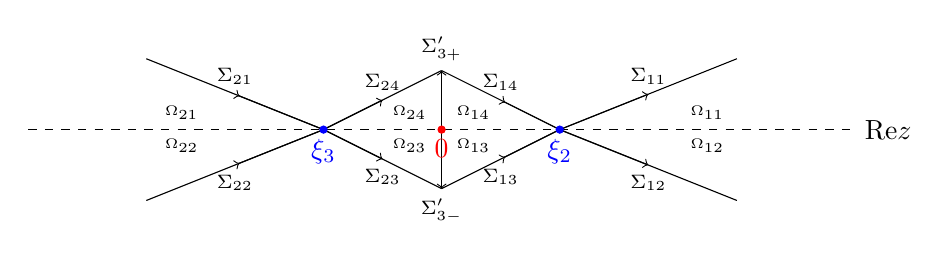
\begin{tikzpicture}[scale=1.5]
                  %\draw(-4,0)--(-5,0.5)node[above]{\scriptsize$\Sigma_{44}$};
                  %\draw[-<](-4,0)--(-4.5,0.25);
                  %\draw(-4,0)--(-2.5,0.6);
                  %\draw[->](-4,0)--(-3.25,-0.3)node[below]{\scriptsize$\Sigma_{42}$};
                  %\draw(-4,0)--(-5,-0.5)node[below]{\scriptsize$\Sigma_{43}$};
                  %\draw[->](-4,0)--(-3.25,0.3)node[above]{\scriptsize$\Sigma_{41}$};
                  %\draw(-4,0)--(-2.5,-0.6);
                  %\draw[-<](-4,0)--(-4.5,-0.25);
      \draw(-1,0)--(0,0.5);
      \draw[->](-1,0)--(-0.5,0.25)node[above]{\scriptsize$\Sigma_{24}$};
      \draw(-1,0)--(-2.5,0.6);
      \draw[-<](-1,0)--(-1.75,-0.3)node[below]{\scriptsize$\Sigma_{22}$};
      \draw(-1,0)--(0,-0.5);
      \draw[-<](-1,0)--(-1.75,0.3)node[above]{\scriptsize$\Sigma_{21}$};
      \draw(-1,0)--(-2.5,-0.6);
      \draw[->](-1,0)--(-0.5,-0.25)node[below]{\scriptsize$\Sigma_{23}$};
      \draw[dashed](-3.5,0)--(3.5,0)node[right]{ Re$z$};
      \draw(1,0)--(0,0.5);
      \draw[-<](1,0)--(0.5,0.25)node[above]{\scriptsize$\Sigma_{14}$};
      \draw(1,0)--(2.5,0.6);
      \draw[->](1,0)--(1.75,-0.3)node[below]{\scriptsize$\Sigma_{12}$};
      \draw(1,0)--(0,-0.5);
      \draw[->](1,0)--(1.75,0.3)node[above]{\scriptsize$\Sigma_{11}$};
      \draw(1,0)--(2.5,-0.6);
      \draw[-<](1,0)--(0.5,-0.25)node[below]{\scriptsize$\Sigma_{13}$};
                  %\draw(4,0)--(5,0.5)node[above]{\scriptsize$\Sigma_{14}$};
                  %\draw[->](4,0)--(4.5,0.25);
                  %\draw(4,0)--(2.5,0.6);
                  %\draw[-<](4,0)--(3.25,-0.3)node[below]{\scriptsize$\Sigma_{12}$};
                  %\draw(4,0)--(5,-0.5)node[below]{\scriptsize$\Sigma_{13}$};
                  %\draw[-<](4,0)--(3.25,0.3)node[above]{\scriptsize$\Sigma_{11}$};
                  %\draw(4,0)--(2.5,-0.6);
                  %\draw[->](4,0)--(4.5,-0.25);
                  %\draw[->](2.5,0)--(2.5,0.6)node[above]{\scriptsize$\Sigma_{2+}'$};
                  %\draw[->](2.5,0)--(2.5,-0.6)node[below]{\scriptsize$\Sigma_{2-}'$};
                  %\draw[->](-2.5,0)--(-2.5,0.6)node[above]{\scriptsize$\Sigma_{4+}'$};
                  %\draw[->](-2.5,0)--(-2.5,-0.6)node[below]{\scriptsize$\Sigma_{4-}'$};
      \draw[->](0,0)--(0,0.5)node[above]{\scriptsize$\Sigma_{3+}'$};
      \draw[->](0,0)--(0,-0.5)node[below]{\scriptsize$\Sigma_{3-}'$};
      \coordinate (I) at (0,0);
      \fill[red] (I) circle (1pt) node[below] {$0$};
                  %\coordinate (A) at (-4,0);
                  %\fill[blue] (A) circle (1pt) node[below] {$\xi_4$};
      \coordinate (b) at (-1,0);
      \fill[blue] (b) circle (1pt) node[below] {$\xi_3$};
                  %\coordinate (e) at (4,0);
                  %\fill[blue] (e) circle (1pt) node[below] {$\xi_1$};
      \coordinate (f) at (1,0);
      \fill[blue] (f) circle (1pt) node[below] {$\xi_2$};
                  %\coordinate (ke) at (4.7,0.1);
                  %\fill (ke) circle (0pt) node[below] {\tiny$\Omega_{13}$};
                  %\coordinate (k1e) at (4.7,-0.1);
                  %\fill (k1e) circle (0pt) node[above] {\tiny$\Omega_{14}$};
                  %\coordinate (le) at (3,0.1);
                  %\fill (le) circle (0pt) node[below] {\tiny$\Omega_{12}$};
                  %\coordinate (l1e) at (3,-0.1);
                  %\fill (l1e) circle (0pt) node[above] {\tiny$\Omega_{11}$};
      \coordinate (n2) at (0.27,0);
      \fill (n2) circle (0pt) node[below] {\tiny$\Omega_{13}$};
      \coordinate (n12) at (0.27,0);
      \fill (n12) circle (0pt) node[above] {\tiny$\Omega_{14}$};
      \coordinate (m2) at (2.25,0);
      \fill (m2) circle (0pt) node[below] {\tiny$\Omega_{12}$};
      \coordinate (m12) at (2.25,0);
      \fill (m12) circle (0pt) node[above] {\tiny$\Omega_{11}$};
                  %\coordinate (k) at (-4.7,0.1);
                  %\fill (k) circle (0pt) node[below] {\tiny$\Omega_{43}$};
                  %\coordinate (k1) at (-4.7,-0.1);
                  %\fill (k1) circle (0pt) node[above] {\tiny$\Omega_{44}$};
                  %\coordinate (l) at (-3,0.1);
                  %\fill (l) circle (0pt) node[below] {\tiny$\Omega_{42}$};
                  %\coordinate (l1) at (-3,-0.1);
                  %\fill (l1) circle (0pt) node[above] {\tiny$\Omega_{41}$};
      \coordinate (n) at (-0.27,0);
      \fill (n) circle (0pt) node[below] {\tiny$\Omega_{23}$};
      \coordinate (n1) at (-0.27,0);
      \fill (n1) circle (0pt) node[above] {\tiny$\Omega_{24}$};
      \coordinate (m) at (-2.2,0);
      \fill (m) circle (0pt) node[below] {\tiny$\Omega_{22}$};
      \coordinate (m1) at (-2.2,0);
      \fill (m1) circle (0pt) node[above] {\tiny$\Omega_{21}$};
                  %\coordinate (c) at (-2,0);
                  %\fill[red] (c) circle (1pt) node[below] {\scriptsize$-1$};
                  %\coordinate (d) at (2,0);
                  %\fill[red] (d) circle (1pt) node[below] {\scriptsize$1$};
   \end{tikzpicture}
   \label{case2}}
   \caption{caption}\label{test}
\end{figure}



\clearpage



\begin{figure}
   \subfigure[]{
   \begin{tikzpicture}[scale=1.2]
      \draw(-4,0)--(-4.8,0.4);
      \draw[dashed](0,2)node[right]{ Im$z$}--(0,-2);
      \draw[-latex](0,2)--(0,2.1);
      \draw[-latex](5.3,0)--(5.4,0);
      \draw[-<](-4,0)--(-4.4,0.2);
      \draw(-4,0)--(-3.2,0.4);
      \draw[->](-4,0)--(-3.6,-0.2);
      \draw(-4,0)--(-4.8,-0.4);
      \draw[->](-4,0)--(-3.6,0.2);
      \draw(-4,0)--(-3.2,-0.4);
      \draw[-<](-4,0)--(-4.4,-0.2);
      \draw(-1,0)--(-0.2,0.4);
      \draw[->](-1,0)--(-0.6,0.2);
      \draw(-1,0)--(-1.8,0.4);
      \draw[-<](-1,0)--(-1.4,-0.2);
      \draw(-1,0)--(-0.2,-0.4);
      \draw[-<](-1,0)--(-1.4,0.2);
      \draw(-1,0)--(-1.8,-0.4);
      \draw[->](-1,0)--(-0.6,-0.2);
      \draw[dashed](-5,0)--(5.4,0)node[right]{ Re$z$};
      \draw(1,0)--(0.2,0.4);
      \draw[-<](1,0)--(0.6,0.2);
      \draw(1,0)--(0.2,-0.4);
      \draw[->](1,0)--(1.4,-0.2);
      \draw(1,0)--(1.8,0.4);
      \draw[->](1,0)--(1.4,0.2);
      \draw(1,0)--(1.8,-0.4);
      \draw[-<](1,0)--(0.6,-0.2);
      \draw(4,0)--(4.8,0.4);
      \draw[->](4,0)--(4.4,0.2);
      \draw(4,0)--(3.2,0.4);
      \draw[-<](4,0)--(3.6,-0.2);
      \draw(4,0)--(4.8,-0.4);
      \draw[-<](4,0)--(3.6,0.2);
      \draw(4,0)--(3.2,-0.4);
      \draw[->](4,0)--(4.4,-0.2);
      \coordinate (I) at (0,0);
      \fill[red] (I) circle (1pt) node[below right] {$0$};
      \coordinate (A) at (-4,0);
      \fill (A) circle (1pt) node[below] {$\xi_4$};
      \coordinate (b) at (-1,0);
      \fill (b) circle (1pt) node[below] {$\xi_3$};
      \coordinate (e) at (4,0);
      \fill (e) circle (1pt) node[below] {$\xi_1$};
      \coordinate (f) at (1,0);
      \fill (f) circle (1pt) node[below] {$\xi_2$};
      \coordinate (c) at (-2,0);
      \fill[red] (c) circle (1pt) node[below] {\scriptsize$-1$};
      \coordinate (d) at (2,0);
      \fill[red] (d) circle (1pt) node[below] {\scriptsize$1$};
   \end{tikzpicture}
   \label{si1}}
   \subfigure[]{
   \begin{tikzpicture}[scale=1.7]
                  %\draw(-4,0)--(-4.8,0.4);
      \draw[dashed](0,1.5)node[right]{ Im$z$}--(0,-1.5);
      \draw[-latex](0,1.5)--(0,1.6);
      \draw[-latex](3.3,0)--(3.4,0);
                  %\draw[-<](-4,0)--(-4.4,0.2);
                  %\draw(-4,0)--(-3.2,0.4);
                  %\draw[->](-4,0)--(-3.6,-0.2);
                  %\draw(-4,0)--(-4.8,-0.4);
                  %\draw[->](-4,0)--(-3.6,0.2);
                  %\draw(-4,0)--(-3.2,-0.4);
                  %\draw[-<](-4,0)--(-4.4,-0.2);
      \draw(-1,0)--(-0.2,0.4);
      \draw[->](-1,0)--(-0.6,0.2);
      \draw(-1,0)--(-1.8,0.4);
      \draw[-<](-1,0)--(-1.4,-0.2);
      \draw(-1,0)--(-0.2,-0.4);
      \draw[-<](-1,0)--(-1.4,0.2);
      \draw(-1,0)--(-1.8,-0.4);
      \draw[->](-1,0)--(-0.6,-0.2);
      \draw[dashed](-3,0)--(3.4,0)node[right]{ Re$z$};
      \draw(1,0)--(0.2,0.4);
      \draw[-<](1,0)--(0.6,0.2);
      \draw(1,0)--(0.2,-0.4);
      \draw[->](1,0)--(1.4,-0.2);
      \draw(1,0)--(1.8,0.4);
      \draw[->](1,0)--(1.4,0.2);
      \draw(1,0)--(1.8,-0.4);
      \draw[-<](1,0)--(0.6,-0.2);
                  %\draw(4,0)--(4.8,0.4);
                  %\draw[->](4,0)--(4.4,0.2);
                  %\draw(4,0)--(3.2,0.4);
                  %\draw[-<](4,0)--(3.6,-0.2);
                  %\draw(4,0)--(4.8,-0.4);
                  %\draw[-<](4,0)--(3.6,0.2);
                  %\draw(4,0)--(3.2,-0.4);
                  %\draw[->](4,0)--(4.4,-0.2);
      \coordinate (I) at (0,0);
      \fill[red] (I) circle (1pt) node[below right] {$0$};
                  %\coordinate (A) at (-4,0);
                  %\fill (A) circle (1pt) node[below] {$\xi_4$};
      \coordinate (b) at (-1,0);
      \fill (b) circle (1pt) node[below] {$\xi_3$};
                  %\coordinate (e) at (4,0);
                  %\fill (e) circle (1pt) node[below] {$\xi_1$};
      \coordinate (f) at (1,0);
      \fill (f) circle (1pt) node[below] {$\xi_2$};
      \coordinate (c) at (-2,0);
      \fill[red] (c) circle (1pt) node[below] {\scriptsize$-1$};
      \coordinate (d) at (2,0);
      \fill[red] (d) circle (1pt) node[below] {\scriptsize$1$};
   \end{tikzpicture}
   \label{si2}}
   \caption{caption}\label{fig-5}
\end{figure}



\clearpage



\begin{figure}
   \centering
   \subfigure[]{
   \begin{tikzpicture}[node distance=3cm]
      \draw[thick](0,0.5)--(3,1)node[above]{$\Sigma_1$};
      \draw[thick](0,0.5)--(-3,1)node[left]{$\Sigma_2$};
      \draw[thick](0,-0.5)--(-3,-1)node[left]{$\Sigma_3$};
      \draw[thick](0,-0.5)--(3,-1)node[right]{$\Sigma_4$};
      \draw[dashed,->](-4,0)--(4,0)node[right]{ Re$z$};
      \draw[dashed,->](0,-2)--(0,2)node[above]{ Im$z$};
      \draw[-latex][thick](0,-0.5)--(-1.5,-0.75);
      \draw[-latex][thick](0,0.5)--(-1.5,0.75);
      \draw[-latex][thick](0,0.5)--(1.5,0.75);
      \draw[-latex][thick](0,-0.5)--(1.5,-0.75);
   \end{tikzpicture}
   }
   \subfigure[]{
   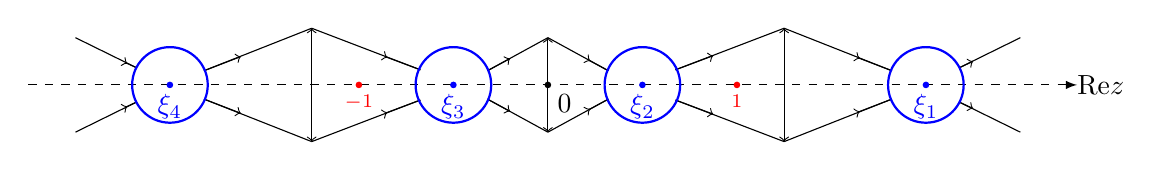
\begin{tikzpicture}[scale=1.2]
      \draw(4.35,0.18)--(5,0.5);
      \draw[->](4.35,0.18)--(4.5,0.25);
      \draw(3.64,0.15)--(2.5,0.6);
      \draw[-<](3.64,-0.15)--(3.25,-0.3);
      \draw(4.35,-0.18)--(5,-0.5);
      \draw[-<](3.64,0.15)--(3.25,0.3);
      \draw(3.64,-0.15)--(2.5,-0.6);
      \draw[->](4.35,-0.18)--(4.5,-0.25);
      \draw(-4.35,0.18)--(-5,0.5);
      \draw[-<](-4.35,0.18)--(-4.5,0.25);
      \draw(-3.64,0.15)--(-2.5,0.6);
      \draw[->](-3.64,-0.15)--(-3.25,-0.3);
      \draw(-4.35,-0.18)--(-5,-0.5);
      \draw[->](-3.64,0.15)--(-3.25,0.3);
      \draw(-3.64,-0.15)--(-2.5,-0.6);
      \draw[-<](-4.35,-0.18)--(-4.5,-0.25);
      \draw(-0.64,0.15)--(0,0.5);
      \draw[->](-0.64,0.15)--(-0.4,0.28);
      \draw(-1.35,0.16)--(-2.5,0.6);
      \draw[-<](-1.35,-0.16)--(-1.75,-0.31);
      \draw(-0.64,-0.15)--(0,-0.5);
      \draw[-<](-1.35,0.16)--(-1.75,0.31);
      \draw(-1.35,-0.16)--(-2.5,-0.6);
      \draw[->](-0.64,-0.15)--(-0.4,-0.28);
      \draw[dashed](-5.5,0)--(5.5,0)node[right]{Re$z$};
      \draw [-latex](5.5,0)--(5.6,0);
      \draw(0.64,0.15)--(0,0.5);
      \draw[-<](0.64,0.15)--(0.4,0.28);
      \draw(1.35,0.16)--(2.5,0.6);
      \draw[->](1.35,-0.16)--(1.75,-0.31);
      \draw(0.64,-0.15)--(0,-0.5);
      \draw[->](1.35,0.16)--(1.75,0.31);
      \draw(1.35,-0.16)--(2.5,-0.6);
      \draw[-<](0.64,-0.15)--(0.4,-0.28);
      \draw[->](2.5,0)--(2.5,0.6);
      \draw[->](2.5,0)--(2.5,-0.6);
      \draw[->](-2.5,0)--(-2.5,0.6);
      \draw[->](-2.5,0)--(-2.5,-0.6);
      \draw[->](0,0)--(0,0.5);
      \draw[->](0,0)--(0,-0.5);
      \coordinate (I) at (0,0);
      \fill (I) circle (1pt) node[below right] {$0$};
      \coordinate (A) at (-4,0);
      \fill[blue] (A) circle (1pt) node[below] {$\xi_4$};
      \coordinate (b) at (-1,0);
      \fill[blue] (b) circle (1pt) node[below] {$\xi_3$};
      \coordinate (e) at (4,0);
      \fill[blue] (e) circle (1pt) node[below] {$\xi_1$};
      \coordinate (f) at (1,0);
      \draw[thick,blue](1,0) circle (0.4);
      \fill[blue] (f) circle (1pt) node[below] {$\xi_2$};
      \draw[thick,blue](4,0) circle (0.4);
      \draw[thick,blue](-1,0) circle (0.4);
      \draw[thick,blue](-4,0) circle (0.4);
      \coordinate (c) at (-2,0);
      \fill[red] (c) circle (1pt) node[below] {\scriptsize$-1$};
      \coordinate (d) at (2,0);
      \fill[red] (d) circle (1pt) node[below] {\scriptsize$1$};
   \end{tikzpicture}
   }
   \subfigure[]{
   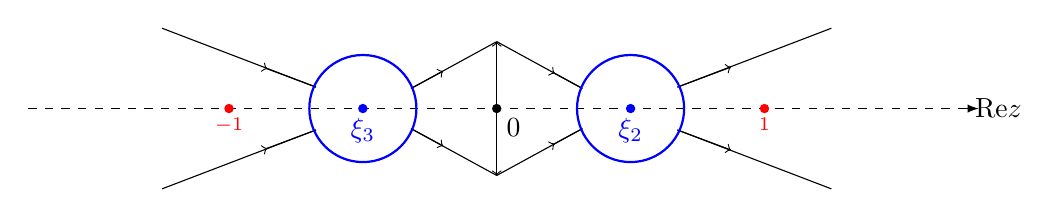
\begin{tikzpicture}[scale=1.7]
                  %\draw(4.35,0.18)--(5,0.5);
                  %\draw[->](4.35,0.18)--(4.5,0.25);
                  %\draw(3.64,0.15)--(2.5,0.6);
                  %\draw[-<](3.64,-0.15)--(3.25,-0.3);
                  %\draw(4.35,-0.18)--(5,-0.5);
                  %\draw[-<](3.64,0.15)--(3.25,0.3);
                  %\draw(3.64,-0.15)--(2.5,-0.6);
                  %\draw[->](4.35,-0.18)--(4.5,-0.25);
                  %\draw(-4.35,0.18)--(-5,0.5);
                  %\draw[-<](-4.35,0.18)--(-4.5,0.25);
                  %\draw(-3.64,0.15)--(-2.5,0.6);
                  %\draw[->](-3.64,-0.15)--(-3.25,-0.3);
                  %\draw(-4.35,-0.18)--(-5,-0.5);
                  %\draw[->](-3.64,0.15)--(-3.25,0.3);
                  %\draw(-3.64,-0.15)--(-2.5,-0.6);
                  %\draw[-<](-4.35,-0.18)--(-4.5,-0.25);
      \draw(-0.64,0.15)--(0,0.5);
      \draw[->](-0.64,0.15)--(-0.4,0.28);
      \draw(-1.35,0.16)--(-2.5,0.6);
      \draw[-<](-1.35,-0.16)--(-1.75,-0.31);
      \draw(-0.64,-0.15)--(0,-0.5);
      \draw[-<](-1.35,0.16)--(-1.75,0.31);
      \draw(-1.35,-0.16)--(-2.5,-0.6);
      \draw[->](-0.64,-0.15)--(-0.4,-0.28);
      \draw[dashed](-3.5,0)--(3.5,0)node[right]{Re$z$};
      \draw [-latex](3.5,0)--(3.6,0);
      \draw(0.64,0.15)--(0,0.5);
      \draw[-<](0.64,0.15)--(0.4,0.28);
      \draw(1.35,0.16)--(2.5,0.6);
      \draw[->](1.35,-0.16)--(1.75,-0.31);
      \draw(0.64,-0.15)--(0,-0.5);
      \draw[->](1.35,0.16)--(1.75,0.31);
      \draw(1.35,-0.16)--(2.5,-0.6);
      \draw[-<](0.64,-0.15)--(0.4,-0.28);
                  %\draw[->](2.5,0)--(2.5,0.6);
                  %\draw[->](2.5,0)--(2.5,-0.6);
                  %\draw[->](-2.5,0)--(-2.5,0.6);
                  %\draw[->](-2.5,0)--(-2.5,-0.6);
      \draw[->](0,0)--(0,0.5);
      \draw[->](0,0)--(0,-0.5);
      \coordinate (I) at (0,0);
      \fill (I) circle (1pt) node[below right] {$0$};
                  %\coordinate (A) at (-4,0);
                  %\fill[blue] (A) circle (1pt) node[below] {$\xi_4$};
      \coordinate (b) at (-1,0);
      \fill[blue] (b) circle (1pt) node[below] {$\xi_3$};
                  %\coordinate (e) at (4,0);
                  %\fill[blue] (e) circle (1pt) node[below] {$\xi_1$};
      \coordinate (f) at (1,0);
      \draw[thick,blue](1,0) circle (0.4);
      \fill[blue] (f) circle (1pt) node[below] {$\xi_2$};
                  %\draw[thick,red](4,0) circle (0.4);
      \draw[thick,blue](-1,0) circle (0.4);
                  %\draw[thick,red](-4,0) circle (0.4);
      \coordinate (c) at (-2,0);
      \fill[red] (c) circle (1pt) node[below] {\scriptsize$-1$};
      \coordinate (d) at (2,0);
      \fill[red] (d) circle (1pt) node[below] {\scriptsize$1$};
   \end{tikzpicture}
   }
   \caption{caption}\label{fig-7}
\end{figure}



\clearpage



\begin{figure}
   \centerline{
   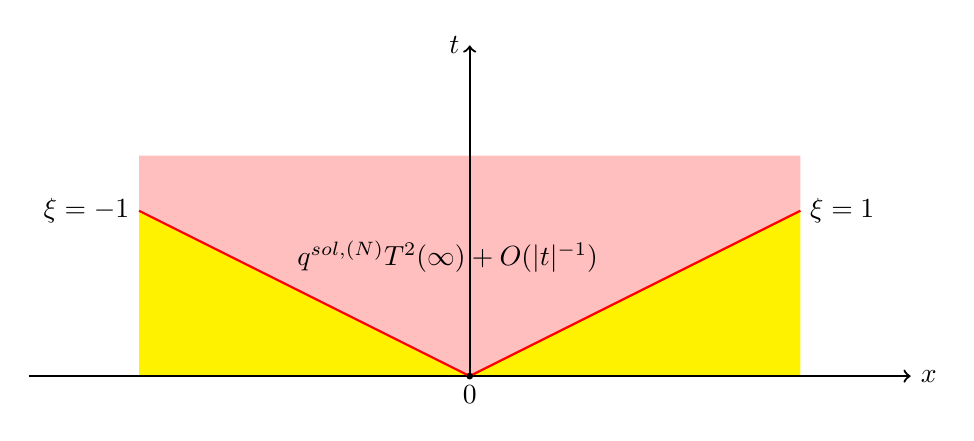
\begin{tikzpicture}[scale=0.7]
      \path [fill=pink] (-6,3)--(-6,4) to (0,4) -- (0,0);
      \path [fill=pink] (0,4)--(0,0) to (6,3) -- (6,4);
      \path [fill=yellow] (-6,0)--(-6,3) to (0,0) -- (0,0);
      \path [fill=yellow] (0,0)--(0,0) to (6,3) -- (6,0);
      \draw[->][thick](-8,0)--(8,0)node[right]{$x$};
      \draw[->][thick](0,0)--(0,6)node[left]{$t$};
      \draw[-][red][thick](0,0)--(6,3);
      \draw[-][red][thick](0,0)--(-6,3);
      \draw[fill] (0,0) circle [radius=0.05];
      \draw[fill] (0,0)node[below]{$0$};
      \draw[fill] (6,3)node[right]{$\xi=1$};
      \draw[fill] (-6,3)node[left]{$\xi=-1$};
      \draw[fill] (-0.4,1.7)node[above]{$q^{sol,(N)}T^2(\infty)+O(|t|^{-1})$};
   \end{tikzpicture}
   }
   \caption{caption}\label{fig01}
\end{figure}



\clearpage



\begin{figure}
   \centerline{
   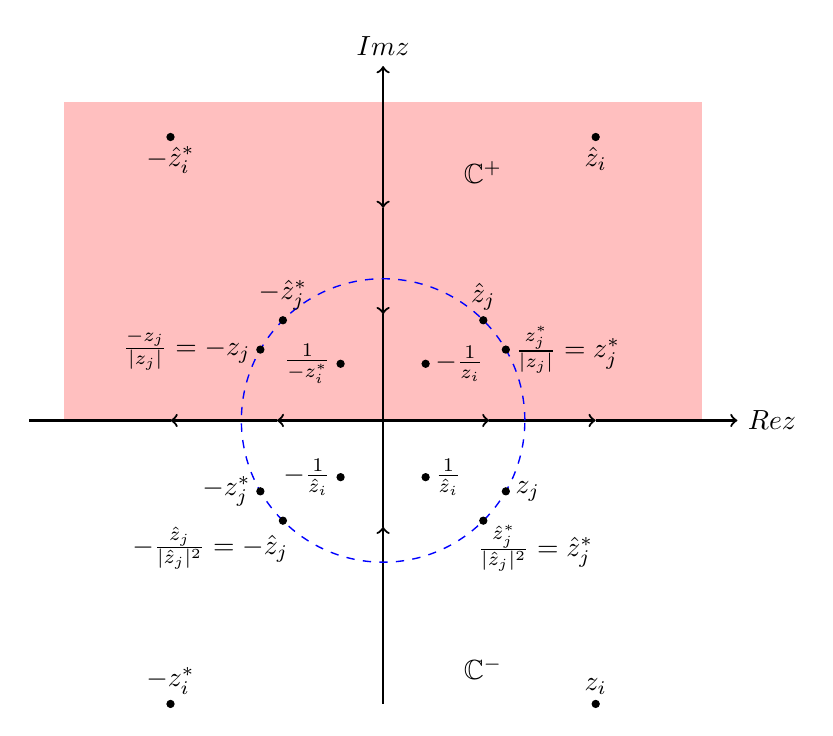
\begin{tikzpicture}[scale=0.9]
      \path [fill=pink] (-4.5,0)--(-4.5,4.5) to (4.5,4.5) -- (4.5,0);
                  %\path [fill=pink] (-5,-4)--(-5,0) to (-1,0) -- (-1,-4);
      \draw[->][thick](3,0)--(5,0)node[right]{$Rez$};
      \draw[->][thick](1.5,0)--(3,0);
      \draw[->][thick](0,0)--(1.5,0);
      \draw[->][thick](0,0)--(-1.5,0);
      \draw[->][thick](-1.5,0)--(-3,0);
      \draw[-][thick](-3,0)--(-5,0);
      \draw[<->][thick](0,3)--(0,5)node[above]{$Imz$};
      \draw[->][thick](0,3)--(0,1.5);
      \draw[-][thick](0,1.5)--(0,0);
      \draw[-][thick](0,-1.5)--(0,0);
      \draw[->][thick](0,-4)--(0,-1.5);
                  %\draw[->][thick](0,-5)--(0,-3);
      \draw(0,0) [dashed][blue, line width=0.5] circle(2);
      \draw[fill] (1.414,1.414) circle [radius=0.05];
      \draw[fill] (1.414,1.414)node[above]{$\hat{z}_{j}$};
      \draw[fill] (-1.414,1.414) circle [radius=0.05];
      \draw[fill] (-1.414,1.414)node[above]{$-\hat{z}^*_{j}$};
      \draw[fill] (1.414,-1.414) circle [radius=0.05];
      \draw[fill] (-1.2,-1.8)node[left]{$-\frac{\hat{z}_{j}}{|\hat{z}_j|^2}=-\hat z_{j}$};
      \draw[fill] (-1.414,-1.414) circle [radius=0.05];
      \draw[fill] (1.2,-1.8)node[right]{$\frac{\hat z^*_{j}}{|\hat{z}_j|^2}=\hat{z}^*_{j}$};
      \draw[fill] (3,4) circle [radius=0.05];
      \draw[fill] (3,4)node[below]{$\hat z_i$};
      \draw[fill] (-3,4) circle [radius=0.05];
      \draw[fill] (-3,4)node[below]{$-\hat z^*_i$};
      \draw[fill] (3,-4) circle [radius=0.05];
      \draw[fill] (3,-4)node[above]{$z_i$};
      \draw[fill] (-3,-4) circle [radius=0.05];
      \draw[fill] (-3,-4)node[above]{$-z^*_i$};
      \draw[fill] (0.6,-0.8) circle [radius=0.05];
      \draw[fill] (0.6,-0.8)node[right]{$\frac{1}{\hat z_i}$};
      \draw[fill] (-0.6,-0.8) circle [radius=0.05];
      \draw[fill] (-0.6,-0.8)node[left]{$-\frac{1}{\hat z_i}$};
      \draw[fill] (1,3.5)node[right]{$\mathbb C^+$};
      \draw[fill] (1,-3.5)node[right]{$\mathbb C^-$};
      \draw[fill] (-0.6,0.8) circle [radius=0.05];
      \draw[fill] (-0.6,0.8)node[left]{$\frac{1}{-z^*_i}$};
      \draw[fill] (0.6,0.8) circle [radius=0.05];
      \draw[fill] (0.6,0.8)node[right]{$-\frac{1}{z_i}$};
      \draw[fill] (1.732,1) circle [radius=0.05];
      \draw[fill] (1.732,1)node[right]{$\frac{z^*_{j}}{|z_{j}|}=z^*_{j}$};
      \draw[fill] (-1.732,1) circle [radius=0.05];
      \draw[fill] (-1.732,1)node[left]{$\frac{-z_{j}}{|z_{j}|}=-z_{j}$};
      \draw[fill] (1.732,-1) circle [radius=0.05];
      \draw[fill] (1.732,-1)node[right]{$z_{j}$};
      \draw[fill] (-1.732,-1) circle [radius=0.05];
      \draw[fill] (-1.732,-1)node[left]{$-z^*_{j}$};
                  %\draw[fill] (4,0)circle [radius=0.05];
                  %\draw[fill] (4.2,0)node[below]{$\xi_{0}$};
                  %\draw[fill] (5.5,0)node[below]{$\xi_{0}+\rho$};
                  %\draw[fill] (2.5,0)node[below]{$\xi_{0}-\rho$};
                  %\draw[-][dashed](3.5,5)--(3.5,-5);
   \end{tikzpicture}
   }
   \caption{caption}\label{fig02}
\end{figure}



\clearpage



\begin{figure}
   \centerline{
   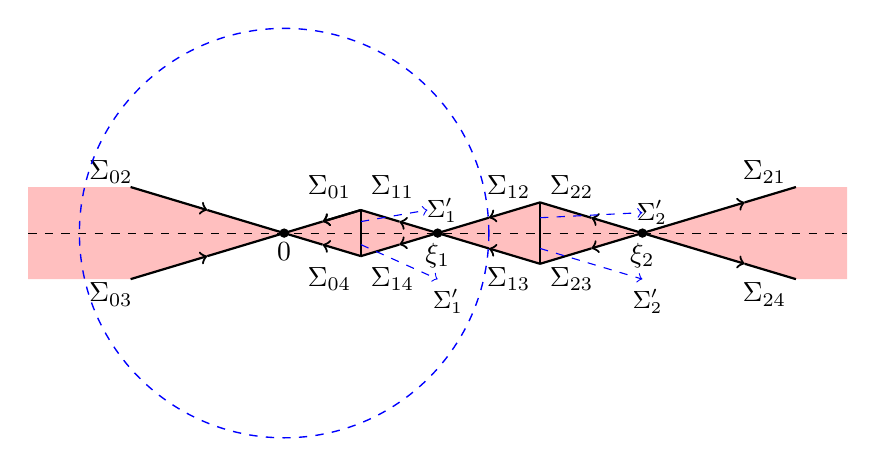
\begin{tikzpicture}[scale=0.65]
      \path [fill=pink] (-3,0) -- (-1.5,0.45) to (0,0) -- (-1.5,-0.45);
      \path [fill=pink] (4,0) -- (2,0.6) to (0,0) -- (2,-0.6);
      \path [fill=pink] (4,0) -- (7,0.9) to (8,0.9) -- (8,0);
      \path [fill=pink] (4,0) -- (7,-0.9) to (8,-0.9) -- (8,0);
      \path [fill=pink] (-3,0) -- (-6,0.9) to (-8,0.9) -- (-8,0);
      \path [fill=pink] (-3,0) -- (-6,-0.9) to (-8,-0.9) -- (-8,0);
      \draw [dashed](-8,0)--(8,0);
      \draw[->][thick](4,0)--(6,0.6);
      \draw[-][thick](6,0.6)--(7,0.9);
      \draw[-][thick](2,0.6)--(2,-0.6);
      \draw[-][thick](-1.5,0.45)--(-1.5,-0.45);
      \draw[->][thick](4,0)--(6,-0.6);
      \draw[-][thick](6,-0.6)--(7,-0.9);
      \draw[->][thick](4,0)--(3,0.3);
      \draw[-][thick](3,0.3)--(2,0.6);
      \draw[->][thick](4,0)--(3,-0.3);
      \draw[-][thick](3,-0.3)--(2,-0.6);
      \draw[->][thick](2,0.6)--(1,0.3);
      \draw[->][thick](1,0.3)--(-0.75,-0.225);
      \draw[->][thick](2,-0.6)--(1,-0.3);
      \draw[->][thick](1,-0.3)--(-0.75,0.225);
      \draw[-][thick](-0.75,0.225)--(-1.5,0.45);
      \draw[->][thick](-1.5,0.45)--(-2.25,0.225);
      \draw[-][thick](-2.25,0.225)--(-4.5,-0.45);
      \draw[->][thick](-1.5,0.45)--(-2.25,0.225);
      \draw[->][thick](-6,0.9)--(-4.5,0.45);
      \draw[-][thick](-0.75,-0.225)--(-1.5,-0.45);
      \draw[->][thick](-1.5,-0.45)--(-2.25,-0.225);
      \draw[-][thick](-2.25,-0.225)--(-4.5,0.45);
      \draw[->][thick](-6,-0.9)--(-4.5,-0.45);
      \draw[fill] (0,0)node[below]{$\xi_1$} circle [radius=0.08];
      \draw[fill] (4,0)node[below]{$\xi_2$} circle [radius=0.08];
      \draw[fill] (-3,0)node[below]{$0$} circle [radius=0.08];
      \draw[fill] (7,1.2)node[left]{$\Sigma_{21}$};
      \draw[fill] (7,-1.2)node[left]{$\Sigma_{24}$};
      \draw[fill] (-7,1.2)node[right]{$\Sigma_{02}$};
      \draw[fill] (-7,-1.2)node[right]{$\Sigma_{03}$};
      \draw[fill] (-1.5,0.9)node[left]{$\Sigma_{01}$};
      \draw[fill] (-1.5,0.9)node[right]{$\Sigma_{11}$};
      \draw[fill] (-1.5,-0.9)node[left]{$\Sigma_{04}$};
      \draw[fill] (-1.5,-0.9)node[right]{$\Sigma_{14}$};
      \draw[fill] (2,0.9)node[left]{$\Sigma_{12}$};
      \draw[fill] (2,0.9)node[right]{$\Sigma_{22}$};
      \draw[fill] (2,-0.9)node[left]{$\Sigma_{13}$};
      \draw[fill] (2,-0.9)node[right]{$\Sigma_{23}$};
      \draw[->][blue,dashed](-1.5,0.225)--(-0.2,0.45);
      \draw[fill] (-0.4,0.45)node[right]{{\small$\Sigma_{1}'$}};
      \draw[->][blue,dashed](-1.5,-0.225)--(0,-0.9);
      \draw[fill] (0.2,-0.9)node[below]{\small{$\Sigma_{1}'$}};
      \draw[->][blue,dashed](2,0.3)--(4,0.4);
      \draw[fill] (3.7,0.4)node[right]{{\small$\Sigma_{2}'$}};
      \draw[->][blue,dashed](2,-0.3)--(4,-0.9);
      \draw[fill] (4.1,-0.9)node[below]{\small{$\Sigma_{2}'$}};
      \draw(-3,0) [dashed][blue, line width=0.5] circle(4);
   \end{tikzpicture}
   }
   
   \caption{caption}\label{fig-2}
\end{figure}



\clearpage



\begin{figure}
   \centerline{
   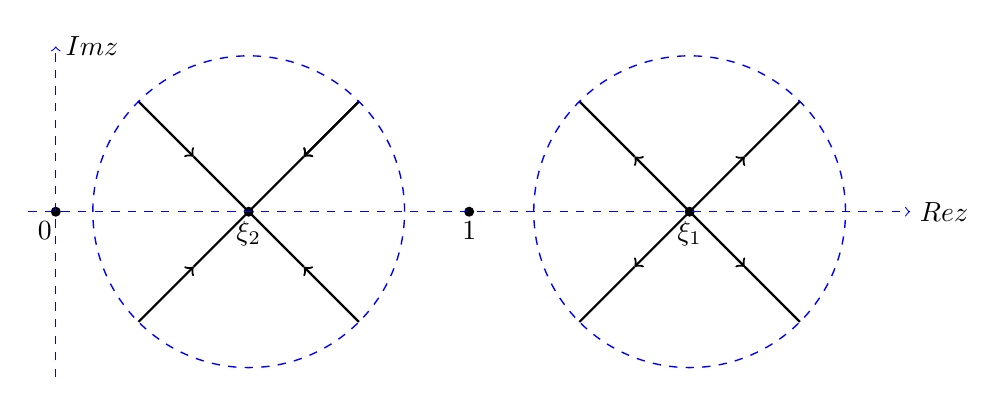
\begin{tikzpicture}[scale=0.7]
      \draw[->][thick](4,0)--(5,1);
      \draw[-][thick](5,1)--(6,2);
      \draw[->][thick](4,0)--(5,-1);
      \draw[-][thick](5,-1)--(6,-2);
      \draw[->][thick](4,0)--(3,1);
      \draw[-][thick](3,1)--(2,2);
      \draw[->][thick](4,0)--(3,-1);
      \draw[-][thick](3,-1)--(2,-2);
      \draw[->][thick](-2,2)--(-3,1);
      \draw[-][thick](-3,1)--(-5,-1);
      \draw[->][thick](-2,2)--(-3,1);
      \draw[->][thick](-6,2)--(-5,1);
      \draw[->][thick](-2,-2)--(-3,-1);
      \draw[-][thick](-3,-1)--(-5,1);
      \draw[->][thick](-6,-2)--(-5,-1);
      \draw[fill] (4,0)node[below]{$\xi_{1}$} circle [radius=0.08];
      \draw[fill] (-4,0)node[below]{$\xi_{2}$} circle [radius=0.08];
      \draw[fill] (0,0)node[below]{$1$} circle [radius=0.08];
      \draw[fill] (-7.5,0) circle [radius=0.08];
      \draw[fill] (-7.7,0)node[below]{$0$};
      \draw[fill] (8,0)node[right]{$Rez$};
      \draw[fill] (-7.5,3)node[right]{$Imz$};
      \draw[->][blue,dashed](-8,0)--(8,0);
      \draw[->][blue,dashed](-7.5,-3)--(-7.5,3);
      \draw(4,0) [dashed][blue, line width=0.5] circle(2.828);
      \draw(-4,0) [dashed][blue, line width=0.5] circle(2.828);
   \end{tikzpicture}
   }
   \caption{caption}\label{fig-5}
\end{figure}



\clearpage



\begin{figure}
   \centerline{
   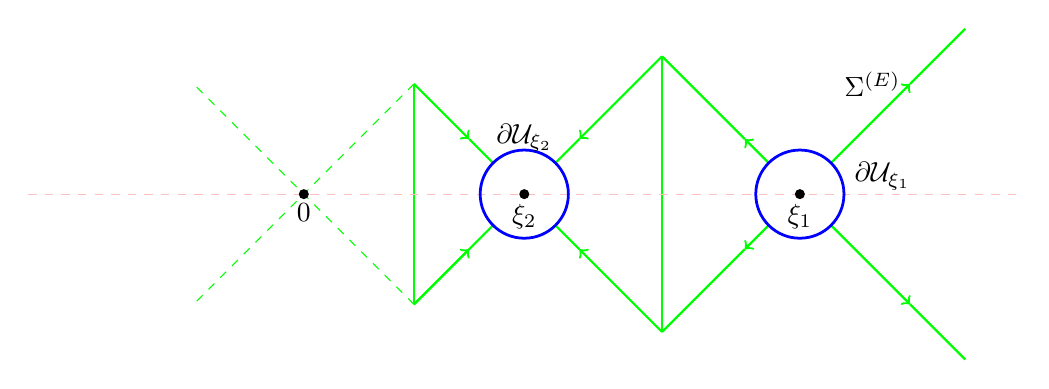
\begin{tikzpicture}[scale=0.7]
      \draw[green, ->][thick](4,0)--(6,2);
      \draw[green,-][thick](6,2)--(7,3);
      \draw[green,->][thick](4,0)--(6,-2);
      \draw[green,-][thick](6,-2)--(7,-3);
      \draw[green,->][thick](4,0)--(3,1);
      \draw[green,-][thick](3,1)--(1.5,2.5);
      \draw[green,->][thick](4,0)--(3,-1);
      \draw[green,-][thick](3,-1)--(1.5,-2.5);
      \draw[green,-][thick](1.5,2.5)--(1.5,-2.5);
                  %\draw[green,->][thick](2,2)--(1,1);
                  %\draw[green,->][thick](1,1)--(-1,-1);
                  %\draw[green,->][thick](2,-2)--(1,-1);
                  %\draw[green,->][thick](1,-1)--(-1,1);
                  %\draw[green,-][thick](-1,1)--(-2,2);
      \draw[green,->][thick](1.5,2.5)--(0,1);
      \draw[green,-][thick](0,1)--(-3,-2);
                  %\draw[green,->][thick](1,2)--(0,1);
      \draw[green,->][thick](-3,2)--(-2,1);
                  %\draw[green,-][thick](2,-1)--(1,-2);
      \draw[green,->][thick](1.5,-2.5)--(0,-1);
      \draw[green,-][thick](0,-1)--(-2,1);
      \draw[green,->][thick](-3,-2)--(-2,-1);
      \draw[green,-][thick](-3,2)--(-3,-2);
      \draw[green,-][dashed](-3,2)--(-7,-2);
      \draw[green,-][dashed](-3,-2)--(-7,2);
      \filldraw[white, line width=0.5](-0.2,0) arc (0:360:0.8);
      \filldraw[white, line width=0.5](4.8,0) arc (-360:0:0.8);
      \draw [pink, dashed](-10,0)--(8,0);
      \draw(4,0) [blue, line width=1] circle(0.8);
      \draw(-1,0) [blue, line width=1] circle(0.8);
      \draw[fill] (-5,0)node[below]{$0$} circle [radius=0.08];
      \draw[fill] (4,0)node[below]{$\xi_1$} circle [radius=0.08];
      \draw[fill] (-1,0)node[below]{$\xi_2$} circle [radius=0.08];
      \draw[fill] (6,2)node[left]{$\Sigma^{(E)}$};
      \draw[fill] (5.5,-0.1)node[above]{$\partial \mathcal{U}_{\xi_1}$};
      \draw[fill] (-1,0.6)node[above]{$\partial \mathcal{U}_{\xi_2}$};
   \end{tikzpicture}
   }
   \caption{caption}\label{fig-7}
\end{figure}



\clearpage



\begin{figure}
   \centerline{
   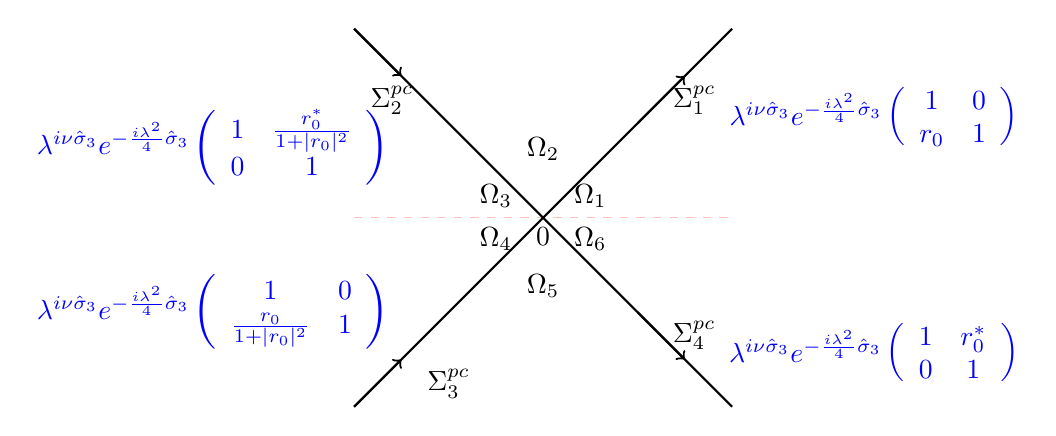
\begin{tikzpicture}[scale=0.6]
      \draw[-][pink,dashed](-4,0)--(4,0);
                  %\draw[-][dashed](-3,0)--(-2,0);
                  %\draw[-][dashed](-2,0)--(-1,0);
                  %\draw[-][dashed](-1,0)--(0,0);
                  %\draw[-][dashed](0,0)--(1,0);
                  %\draw[-][dashed](1,0)--(2,0);
                  %\draw[-][dashed](2,0)--(3,0);
                  %\draw[-][dashed](3,0)--(4,0);
                  %\draw[-][thick](0,4)--(0,3);
                  %\draw[-][thick](0,3)--(0,2);
                  %\draw[-][thick](0,2)--(0,1);
                  %\draw[-][thick](0,1)--(0,0);
                  %\draw[-][thick](0,-4)--(0,-3);
                  %\draw[-][thick](0,-3)--(0,-2);
                  %\draw[-][thick](0,-2)--(0,-1);
                  %\draw[-][thick](0,-1)--(0,-0);
      \draw[-][thick](-4,-4)--(4,4);
      \draw[-][thick](-4,4)--(4,-4);
      \draw[->][thick](2,2)--(3,3);
      \draw[->][thick](-4,4)--(-3,3);
      \draw[->][thick](-4,-4)--(-3,-3);
      \draw[->][thick](2,-2)--(3,-3);
      \draw[fill] (3.2,3)node[below]{$\Sigma_{1}^{pc}$};
      \draw[fill] (3.2,-3)node[above]{$\Sigma_{4}^{pc}$};
      \draw[fill] (-3.2,3)node[below]{$\Sigma_{2}^{pc}$};
      \draw[fill] (-2,-3)node[below]{$\Sigma_{3}^{pc}$};
      \draw[fill] (0,0)node[below]{$0$};
      \draw[fill] (1,0)node[below]{$\Omega_{6}$};
      \draw[fill] (1,0)node[above]{$\Omega_{1}$};
      \draw[fill] (0,-1)node[below]{$\Omega_{5}$};
      \draw[fill] (0,1)node[above]{$\Omega_{2}$};
      \draw[fill] (-1,0)node[below]{$\Omega_{4}$};
      \draw[fill] (-1,0)node[above]{$\Omega_{3}$};
      \draw[fill] (7,3)node[blue,below]{$\lambda^{i\nu\hat{\sigma}_{3}}e^{-\frac{i\lambda^{2}}{4}\hat{\sigma}_{3}}
      \left(
      \begin{array}{cc}
         1 & 0 \\
         r_{0} & 1 \\
      \end{array}
      \right)
      $};
      \draw[blue,fill] (7,-2)node[below]{$\lambda^{i\nu\hat{\sigma}_{3}}e^{-\frac{i\lambda^{2}}{4}\hat{\sigma}_{3}}
      \left(
      \begin{array}{cc}
         1 & r^{*}_{0} \\
         0 & 1 \\
      \end{array}
      \right)
      $};
      \draw[blue,fill] (-7,2.5)node[below]{$\lambda^{i\nu\hat{\sigma}_{3}}e^{-\frac{i\lambda^{2}}{4}\hat{\sigma}_{3}}
      \left(
      \begin{array}{cc}
         1 & \frac{r^{*}_{0}}{1+|r_{0}|^{2}} \\
         0 & 1 \\
      \end{array}
      \right)
      $};
      \draw[blue,fill] (-7,-1)node[below]{$\lambda^{i\nu\hat{\sigma}_{3}}e^{-\frac{i\lambda^{2}}{4}\hat{\sigma}_{3}}
      \left(
      \begin{array}{cc}
         1 & 0 \\
         \frac{r_{0}}{1+|r_{0}|^{2}} & 1 \\
      \end{array}
      \right)
      $};
   \end{tikzpicture}
   }
   \caption{caption}\label{fig-6}
\end{figure}



\clearpage



\begin{figure}
   \begin{center}
      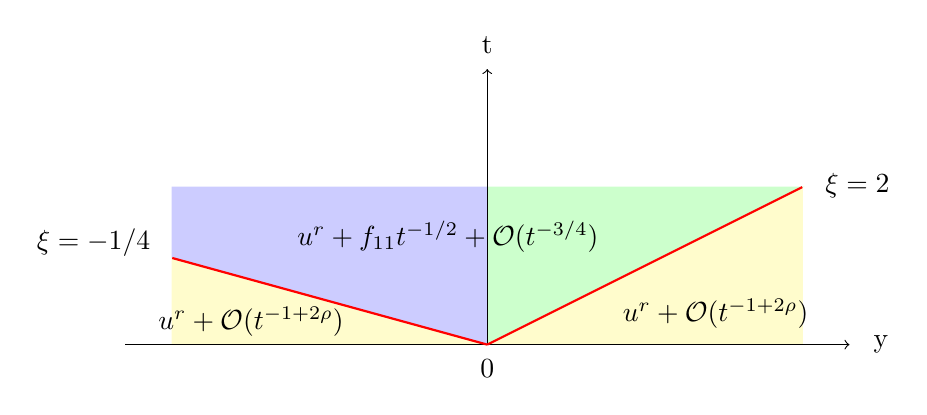
\begin{tikzpicture}
         \draw[yellow!20, fill=yellow!20] (0,0)--(4,0)--(4,2)--(0, 2);
         \draw[green!20, fill=green!20] (0,0 )--(4,2)--(0,2)--(0,0);
         \draw[blue!20, fill=blue!20] (0,0 )--(-4,1.1)--(-4,2)--(0, 2)--(0,0);
         \draw[yellow!20, fill=yellow!20] (0,0 )--(-4,0)--(-4,1.1)--(0,0);
         \draw [ -> ] (-4.6,0)--(4.6,0);
         \draw [ -> ](0,0)--(0,3.5);
         \draw [red,thick  ](0,0 )--(4,2);
         \draw [red,thick  ](0,0 )--(-4,1.1);
         \node    at (0,-0.3)  {$0$};
         \node    at (5,0)  {y};
         \node    at (0,3.8 )  {t};
         \node  [below]  at (-0.5,1.7) {$u^r  +f_{11}t^{-1/2}+\mathcal{O}(t^{-3/4})$};
                           %\node  [below]  at (-1.5,1.8) {$-1/4<\xi<0 $};
         \node  [below]  at (2.9,0.7) {$  u^r +\mathcal{O}(t^{-1+2\rho})$};
         \node  [below]  at (-3,0.6) {$     u^r +\mathcal{O}(t^{-1+2\rho}) $};
         \node  [below]  at (-5,1.6) {$ \xi=-1/4 $};
         \node  [below]  at (4.7,2.3) {$ \xi=2 $};
      \end{tikzpicture}
   \end{center}
   \caption{caption}\label{result1}
\end{figure}



\clearpage



\begin{figure}
   \centerline{
   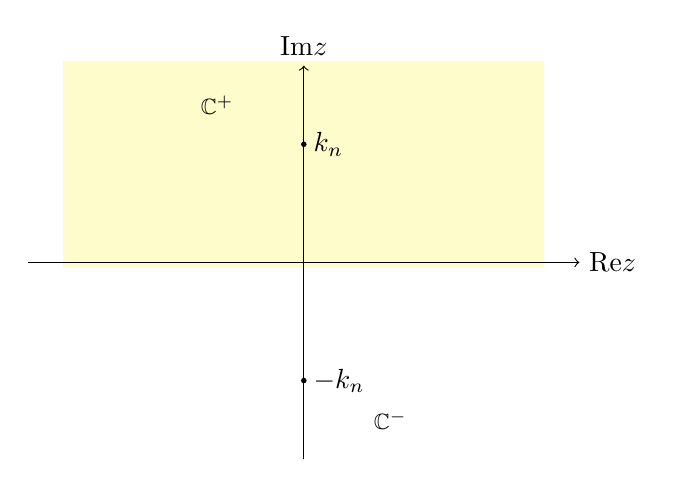
\begin{tikzpicture}[node distance=2cm]
      \filldraw[yellow!20,line width=3] (3,0) rectangle (0,2.5);
      \filldraw[yellow!20,line width=3] (-3,0) rectangle (-0,2.5);
                  %\filldraw[green!20,line width=3] (3,0) rectangle (0,-3);
                  %\filldraw[green!20,line width=3] (-3,0) rectangle (-0,-3);
      \draw[->](-3.5,0)--(3.5,0)node[right]{Re$z$};
      \draw[->](0,-2.5)--(0,2.5)node[above]{Im$z$};
      \node   at (-1.1,2) {\footnotesize $\mathbb{C}^+$};
      \node   at (1.1,-2) {\footnotesize $\mathbb{C}^-$};
      \coordinate (A) at (0,1.5);
      \coordinate (B) at (0,-1.5);
      
      \fill (A) circle (1pt) node[right] {$k_n$};
      \fill (B) circle (1pt) node[right] {$-k_n$};
   \end{tikzpicture}
   }
   \caption{caption}\label{fig:figure2}
\end{figure}



\clearpage



\begin{figure}
   \begin{center}
      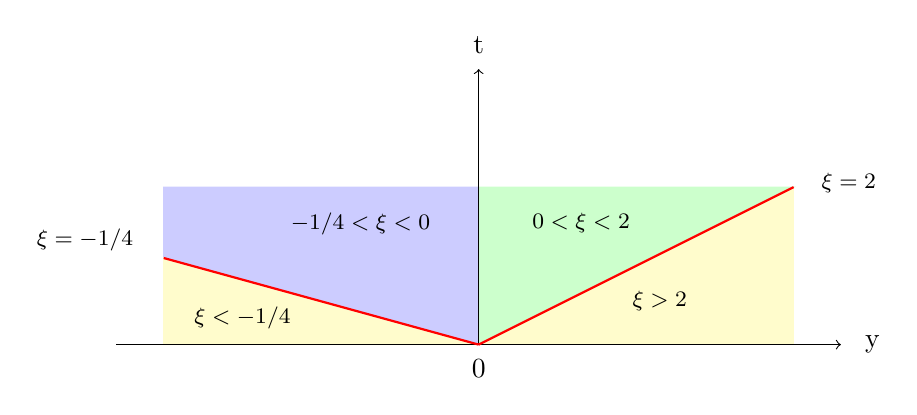
\begin{tikzpicture}
         \draw[yellow!20, fill=yellow!20] (0,0)--(4,0)--(4,2)--(0, 2);
         \draw[green!20, fill=green!20] (0,0 )--(4,2)--(0,2)--(0,0);
         \draw[blue!20, fill=blue!20] (0,0 )--(-4,1.1)--(-4,2)--(0, 2)--(0,0);
         \draw[yellow!20, fill=yellow!20] (0,0 )--(-4,0)--(-4,1.1)--(0,0);
         \draw [ -> ] (-4.6,0)--(4.6,0);
         \draw [ -> ](0,0)--(0,3.5);
         \draw [red,thick  ](0,0 )--(4,2);
         \draw [red,thick  ](0,0 )--(-4,1.1);
         \node    at (0,-0.3)  {$0$};
         \node    at (5,0)  {y};
         \node    at (0,3.8 )  {t};
         \node  [below]  at (1.3,1.8) {\footnotesize $0<\xi<2$};
         \node  [below]  at (-1.5,1.8) {\footnotesize $-1/4<\xi<0 $};
         \node  [below]  at (2.3,0.8) {\footnotesize $ \xi>2$};
         \node  [below]  at (-3,0.6) {\footnotesize $ \xi<-1/4 $};
         \node  [below]  at (-5,1.6) {\footnotesize $ \xi=-1/4 $};
         \node  [below]  at (4.7,2.3) {\footnotesize $ \xi=2 $};
      \end{tikzpicture}
   \end{center}
   \caption{caption}\label{regions1}
\end{figure}



\clearpage



\begin{figure}
   \begin{center}
      \subfigure[]{
      \begin{tikzpicture}
         \draw[->, red](-5.5,0)--(5.5,0)node[right]{ \textcolor{black}{Re$z$}};
         \draw[->, red](0,-1.5)--(0,1.5)node[right]{\textcolor{black}{Im$z$}};
         \coordinate (I) at (0,0);
         \fill (I) circle (1pt) node[below] {$0$};
         \coordinate (A) at (-4,0);
         \fill (A) circle (1pt) node[blue,below] {$\xi_4$};
         \coordinate (b) at (-2,0);
         \fill (b) circle (1pt) node[blue,below] {$\xi_3$};
         \coordinate (e) at (4,0);
         \fill (e) circle (1pt) node[blue,below] {$\xi_1$};
         \coordinate (f) at (2,0);
         \fill (f) circle (1pt) node[blue,below] {$\xi_2$};
      \end{tikzpicture}
      \label{pcase1}}
      \subfigure[]{
      \begin{tikzpicture}
         \draw[->,red](-5.5,0)--(5.5,0) node[right] {\textcolor{black}{ Re$z$}};
         \draw[->,red](0,-1.5)--(0,1.5)node[right]{\textcolor{black}{Im$z$}};
         \coordinate (I) at (0,0);
         \fill (I) circle (1pt) node[below] {$0$};
         \coordinate (E) at (3,0);
         \fill (E) circle (1pt) node[blue,below] {$\xi_1$};
         \coordinate (R) at (-3,0);
         \fill (R) circle (1pt) node[blue,below] {$\xi_2$};
      \end{tikzpicture}
      \label{phase2}}
      \caption{caption}\label{phase}
   \end{center}
\end{figure}



\clearpage



\begin{figure}
   \centering
   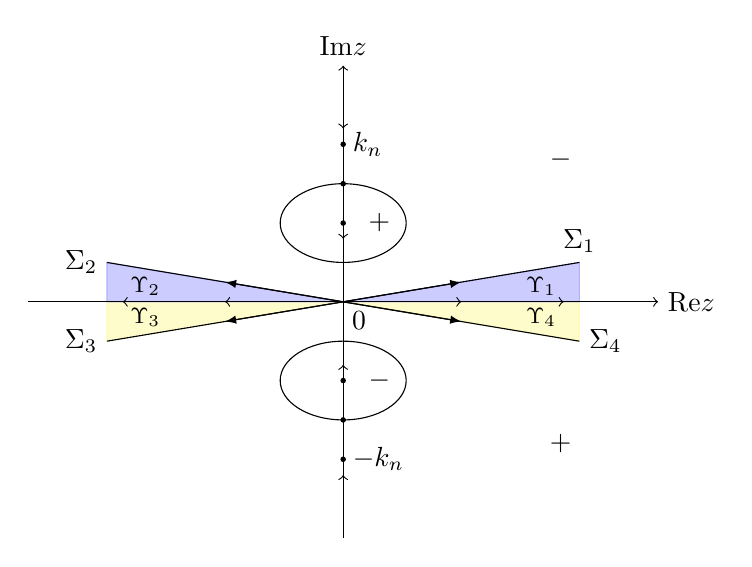
\begin{tikzpicture}[node distance=2cm]
      \draw[yellow!30, fill=yellow!20] (0,0)--(3,-0.5)--(3,0)--(0,0)--(-3,-0.5)--(-3,0)--(0,0);
      \draw[blue!30, fill=blue!20] (0,0)--(3,0.5)--(3,0)--(0,0)--(-3, 0.5)--(-3,0)--(0,0);
      \draw(0,0)--(3,0.5)node[above]{$\Sigma_1$};
      \draw(0,0)--(-3,0.5)node[left]{$\Sigma_2$};
      \draw(0,0)--(-3,-0.5)node[left]{$\Sigma_3$};
      \draw(0,0)--(3,-0.5)node[right]{$\Sigma_4$};
      \draw[->](-4,0)--(4,0)node[right]{ Re$z$};
      \draw[->](0,-3)--(0,3)node[above]{ Im$z$};
      \draw[-latex](0,0)--(-1.5,-0.25);
      \draw[-latex](0,0)--(-1.5,0.25);
      \draw[-latex](0,0)--(1.5,0.25);
      \draw[-latex](0,0)--(1.5,-0.25);
      \coordinate (C) at (-0.2,2.2);
      \coordinate (D) at (2.2,0.2);
      \fill (D) circle (0pt) node[right] {\footnotesize $\Upsilon_1$};
      \coordinate (J) at (-2.2,-0.2);
      \fill (J) circle (0pt) node[left] {\footnotesize $\Upsilon_3$};
      \coordinate (k) at (-2.2,0.2);
      \fill (k) circle (0pt) node[left] {\footnotesize $\Upsilon_2$};
      \coordinate (k) at (2.2,-0.2);
      \fill (k) circle (0pt) node[right] {\footnotesize $\Upsilon_4$};
      \coordinate (I) at (0.2,0);
      \fill (I) circle (0pt) node[below] {$0$};
      \draw[  ][->](0,0)--(-1.5,0);
      \draw[ ][->](-1.5,0)--(-2.8,0);
      \draw[ ][->](0,0)--(1.5,0);
      \draw[ ][->](1.5,0)--(2.8,0);
      \draw[ ][->](0,2.7)--(0,2.2);
      \draw[ ][->](0,1.6)--(0,0.8);
      \draw[ ][->](0,-2.7)--(0,-2.2);
      \draw[ ][->](0,-1.6)--(0,-0.8);
      \draw[ ](0,1) ellipse (0.8 and 0.5);
      \draw[ ](0,-1) ellipse (0.8 and 0.5);
      \coordinate (A) at (0.2,1);
      \fill (A) circle (0pt) node[right] {$+$};
      \coordinate (B) at (0.2,-1);
      \fill (B) circle (0pt) node[right] {$-$};
      \coordinate (C) at (2.5,1.8);
      \fill (C) circle (0pt) node[right] {$-$};
      \coordinate (D) at (2.5,-1.8);
      \fill (D) circle (0pt) node[right] {$+$};
      \coordinate (E) at (0,1.5);
      \fill (E) circle (1pt) ;
      \coordinate (F) at (0,-1.5);
      \fill (F) circle (1pt) ;
      \coordinate (G) at (0,-2);
      \fill (G) circle (1pt)node[right] {$-k_n$}; %node[right] {$-k_n$};
      \coordinate (H) at (0,2);
      \fill (H) circle (1pt) node[right] {$k_n$}; %node[right] {$\bar{k}_n$};
      \coordinate (I) at (0,1);
      \fill (I) circle (1pt) ;
      \coordinate (J) at (0,-1);
      \fill (J) circle (1pt) ;
                         % \coordinate (K) at (0.18,-1);
                          %\fill (K) circle (1pt) ;
                         % \coordinate (L) at (-0.18,-1);
                          %\fill (L) circle (1pt) ;
                          %\coordinate (M) at (0.613,0.679);
                          %\fill (M) circle (1pt) ;
                         % \coordinate (N) at (-0.613,0.679);
                         % \fill (N) circle (1pt) ;
                          %\coordinate (O) at (0.613,-0.679);
                          %\fill (O) circle (1pt) ;
                         % \coordinate (P) at (-0.613,-0.679);
                          %\fill (P) circle (1pt) ;
                  %\coordinate (F) at (0.5546996232,-0.8320505887);
                  %\coordinate (G) at (-2,3);
                  %\coordinate (H) at (-2,-3);
                  %\coordinate (K) at (1.7320508075688774,-1);
                  %\coordinate (L) at (-1.7320508075688774,1);
                  %\coordinate (M) at (-1.7320508075688774,-1);
      
                  %\fill (F) circle (1pt) node[right] {$\frac{1}{z_n}$};
                  %\fill (G) circle (1pt) node[left] {$-\bar{z}_n$};
                  %\fill (H) circle (1pt) node[left] {$-z_n$};
                  %\fill (J) circle (1pt) node[right] {$w_m$};
                  %\fill (K) circle (1pt) node[right] {$\bar{w}_m$};
                  %\fill (M) circle (1pt) node[left] {$-w_m$};
   \end{tikzpicture}
   \caption{caption}\label{figR2}
\end{figure}



\clearpage



\begin{figure}
   \centering
   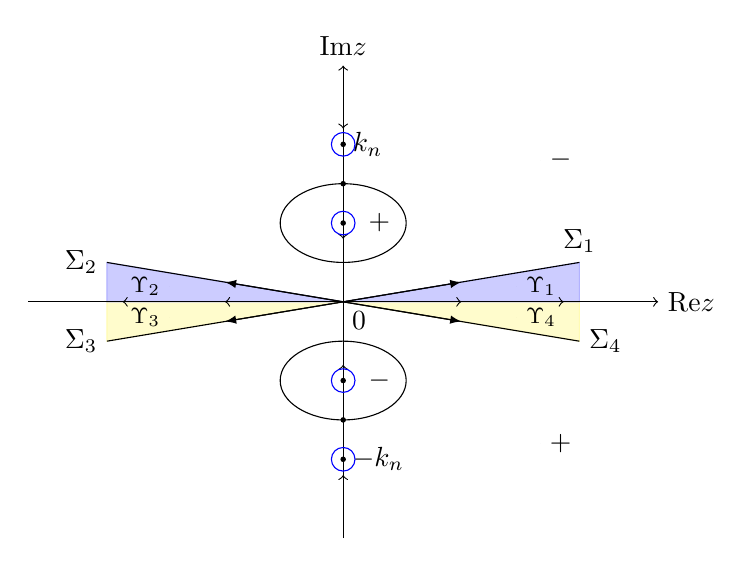
\begin{tikzpicture}[node distance=2cm]
      \draw[yellow!30, fill=yellow!20] (0,0)--(3,-0.5)--(3,0)--(0,0)--(-3,-0.5)--(-3,0)--(0,0);
      \draw[blue!30, fill=blue!20] (0,0)--(3,0.5)--(3,0)--(0,0)--(-3, 0.5)--(-3,0)--(0,0);
      \draw(0,0)--(3,0.5)node[above]{$\Sigma_1$};
      \draw(0,0)--(-3,0.5)node[left]{$\Sigma_2$};
      \draw(0,0)--(-3,-0.5)node[left]{$\Sigma_3$};
      \draw(0,0)--(3,-0.5)node[right]{$\Sigma_4$};
      \draw[->](-4,0)--(4,0)node[right]{ Re$z$};
      \draw[->](0,-3)--(0,3)node[above]{ Im$z$};
      \draw[-latex](0,0)--(-1.5,-0.25);
      \draw[-latex](0,0)--(-1.5,0.25);
      \draw[-latex](0,0)--(1.5,0.25);
      \draw[-latex](0,0)--(1.5,-0.25);
      \coordinate (C) at (-0.2,2.2);
      \coordinate (D) at (2.2,0.2);
      \fill (D) circle (0pt) node[right] {\footnotesize $\Upsilon_1$};
      \coordinate (J) at (-2.2,-0.2);
      \fill (J) circle (0pt) node[left] {\footnotesize $\Upsilon_3$};
      \coordinate (k) at (-2.2,0.2);
      \fill (k) circle (0pt) node[left] {\footnotesize $\Upsilon_2$};
      \coordinate (k) at (2.2,-0.2);
      \fill (k) circle (0pt) node[right] {\footnotesize $\Upsilon_4$};
      \coordinate (I) at (0.2,0);
      \fill (I) circle (0pt) node[below] {$0$};
      \draw[  ][->](0,0)--(-1.5,0);
      \draw[ ][->](-1.5,0)--(-2.8,0);
      \draw[ ][->](0,0)--(1.5,0);
      \draw[ ][->](1.5,0)--(2.8,0);
      \draw[ ][->](0,2.7)--(0,2.2);
      \draw[ ][->](0,1.6)--(0,0.8);
      \draw[ ][->](0,-2.7)--(0,-2.2);
      \draw[ ][->](0,-1.6)--(0,-0.8);
      \draw[ ](0,1) ellipse (0.8 and 0.5);
      \draw[ ](0,-1) ellipse (0.8 and 0.5);
      \coordinate (A) at (0.2,1);
      \fill (A) circle (0pt) node[right] {$+$};
      \coordinate (B) at (0.2,-1);
      \fill (B) circle (0pt) node[right] {$-$};
      \coordinate (C) at (2.5,1.8);
      \fill (C) circle (0pt) node[right] {$-$};
      \coordinate (D) at (2.5,-1.8);
      \fill (D) circle (0pt) node[right] {$+$};
      \coordinate (E) at (0,1.5);
      \fill (E) circle (1pt) ;
      \coordinate (F) at (0,-1.5);
      \fill (F) circle (1pt) ;
      \coordinate (G) at (0,-2);
      \fill (G) circle (1pt)node[right] {$-k_n$}; %node[right] {$-k_n$};
      \coordinate (H) at (0,2);
      \fill (H) circle (1pt) node[right] {$k_n$}; %node[right] {$\bar{k}_n$};
      \coordinate (I) at (0,1);
      \fill (I) circle (1pt) ;
      \coordinate (J) at (0,-1);
      \fill (J) circle (1pt) ;
      \draw[blue] (0,2) circle (0.15);
      \draw[blue] (0,-2) circle (0.15);
      \draw[blue] (0,1) circle (0.15);
      \draw[blue] (0,-1) circle (0.15);
                          %\fill (K) circle (1pt) ;
                         % \coordinate (L) at (-0.18,-1);
                          %\fill (L) circle (1pt) ;
                          %\coordinate (M) at (0.613,0.679);
                          %\fill (M) circle (1pt) ;
                         % \coordinate (N) at (-0.613,0.679);
                         % \fill (N) circle (1pt) ;
                          %\coordinate (O) at (0.613,-0.679);
                          %\fill (O) circle (1pt) ;
                         % \coordinate (P) at (-0.613,-0.679);
                          %\fill (P) circle (1pt) ;
                  %\coordinate (F) at (0.5546996232,-0.8320505887);
                  %\coordinate (G) at (-2,3);
                  %\coordinate (H) at (-2,-3);
                  %\coordinate (K) at (1.7320508075688774,-1);
                  %\coordinate (L) at (-1.7320508075688774,1);
                  %\coordinate (M) at (-1.7320508075688774,-1);
      
                  %\fill (F) circle (1pt) node[right] {$\frac{1}{z_n}$};
                  %\fill (G) circle (1pt) node[left] {$-\bar{z}_n$};
                  %\fill (H) circle (1pt) node[left] {$-z_n$};
                  %\fill (J) circle (1pt) node[right] {$w_m$};
                  %\fill (K) circle (1pt) node[right] {$\bar{w}_m$};
                  %\fill (M) circle (1pt) node[left] {$-w_m$};
   \end{tikzpicture}
   \caption{caption}\label{figVR}
\end{figure}



\clearpage



\begin{figure}
   \begin{center}
      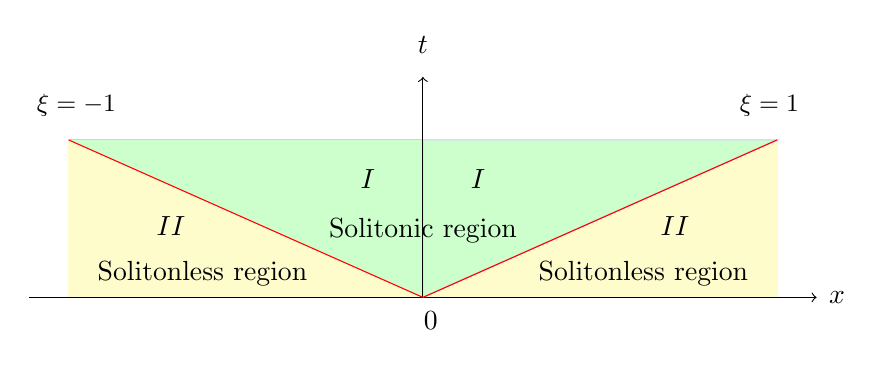
\begin{tikzpicture}
         \draw[yellow!20, fill=yellow!20] (0,0)--(4.5,0)--(4.5,2)--(0, 2);
         \draw[blue!20, fill=green!20] (0,0 )--(4.5,2)--(0,2)--(0,0);
         \draw[blue!20, fill=green!20] (0,0 )--(-4.5,0)--(-4.5,2)--(0, 2)--(0,0);
         \draw[yellow!20, fill=yellow!20] (0,0 )--(-4.5,0)--(-4.5,2)--(0,0);
                           %\draw[CadetBlue!20, fill=LightSteelBlue!20] (0,0)--(2.5,0)--(2.5,2)--(0, 2);
                           %\draw[CadetBlue!20, fill=LightSteelBlue!20] (-2.5,0)--(0,0)--(0,2)--(-2.5, 2);
                           %\draw[GreenYellow!20, fill=YellowGreen!20] (-2.5,-2)--(0,-2)--(0,0)--(-2.5, 0);
                           %\draw[GreenYellow!20, fill=YellowGreen!20] (0,-2)--(2.5,-2)--(2.5,0)--(0, 0);
                           %\draw[CadetBlue!20, fill=LightSteelBlue!20] (-3.5,2.5)--(0,0)--(3.5,2.5);
                           %\draw[GreenYellow!20, fill=LightSteelBlue!] (-3.5,2.5)--(-3.5,0)--(0,0);
                           %\draw[GreenYellow!20, fill=LightSteelBlue!] (3.5,2.5)--(3.5,0)--(0,0);
         \draw [-> ](-5,0)--(5,0);
         \draw [-> ](0,0)--(0,2.8);
         \node    at (0.1,-0.3)  {$0$};
         \node    at (5.26,0)  { $x$};
         \node    at (0,3.2)  { $t$};
                           %\draw [dashed](0,0)--(-4,2);
                           %\draw [dashed](0,0)--(4,2);
         \node  [below]  at (4.4,2.7) {\small$\xi=1$};
         \node  [below]  at (-4.4,2.7) {\small$\xi=-1$};
                           %\node at (-0.1,1.5) {\small$|x/t|<2$};
         \draw [red](0,0)--(-4.5,2);
         \draw [red](0,0)--(4.5,2);
                           %\node  []  at (4,0.8) {\small$\xi=K$};
                           %\node  []  at (-4,0.8) {\small$\xi=-K$};
         \node  []  at (0.7,1.5) { $I$};
         \node  []  at (-0.7,1.5) { $I$};
         \node [] at (0,0.85) {Solitonic region};
         \node  []  at (-3.2,0.9) { $II$};
         \node [] at (-2.8,0.3) {Solitonless region};
         \node  []  at (3.2,0.9) { $II$};
         \node [] at (2.8,0.3) {Solitonless region};
      \end{tikzpicture}
   \end{center}
   \caption{caption}\label{spacetime}
\end{figure}



\clearpage



\begin{figure}
   \begin{center}
      \begin{tikzpicture}
                           %\draw[CadetBlue!20, fill=LightSteelBlue!20] (0,0)--(2.5,0)--(2.5,2)--(0, 2);
                           %\draw[CadetBlue!20, fill=LightSteelBlue!20] (-2.5,0)--(0,0)--(0,2)--(-2.5, 2);
                           %\draw[GreenYellow!20, fill=YellowGreen!20] (-2.5,-2)--(0,-2)--(0,0)--(-2.5, 0);
                           %\draw[GreenYellow!20, fill=YellowGreen!20] (0,-2)--(2.5,-2)--(2.5,0)--(0, 0);
         \draw [-> ](-3.5,0)--(3.5,0);
         \draw [-> ](0,-2.8)--(0,2.8);
         \node    at (0.3,-0.3)  {$0$};
         \node    at (4,0)  { Re$z$};
         \node    at (0,3.2)  { Im$z$};
         \node  [below]  at (1.3,1.2) {$\mathbb{C}^+$};
         \node  [below]  at (-1.2,1.2) {$\mathbb{C}^+$};
         \node  [below]  at (-1.2,-0.8) {$\mathbb{C}^-$};
         \node  [below]  at (1.3,-0.8) {$\mathbb{C}^-$};
      \end{tikzpicture}
   \end{center}
   \caption{caption}\label{analytic}
\end{figure}



\clearpage



\begin{figure}
   \begin{center}
      \begin{tikzpicture}[node distance=2cm]
         \draw[->](-4,0)--(4,0)node[black,right]{Re$z$};
         \foreach \x [count=\p] in {0,...,11} {
         \node[shape=circle,fill=red, scale=0.25] (\p) at (-\x*30:2) {};};
         \foreach \x [count=\p] in {0,...,5} {
         \draw (-\x*60:2.4) ;
         \draw (-30-\x*60:2.4) ;};
         \node[shape=circle,fill=blue, scale=0.15]  at (0:2){0};
         \node[shape=circle,fill=blue, scale=0.15]  at (-6*30:2){0} ;
         \node[shape=circle,fill=blue,scale=0.15] at (0,0) {0};
         \node[below] at (2.1,0) {$1$};
         \node[below] at (0,0) {$0$};
         \node[below] at (-2.2,0) {$-1$};
         \node[right] at (1*30:2) {$z_j$};
         \node[right] at (-1*30:2) {$\bar{z}_j$};
                           %  \node[left] at (5*30:2) {$\bar{z}_k$};
                           %  \node[left] at (-5*30:2) {$z_j$};
         \draw [dashed, gray](1) arc (0:360:2);
      \end{tikzpicture}
      \caption{caption}\label{mjumpp}
   \end{center}
\end{figure}



\clearpage



\begin{figure}
   \begin{center}
      \subfigure[$ \xi>1$]{
      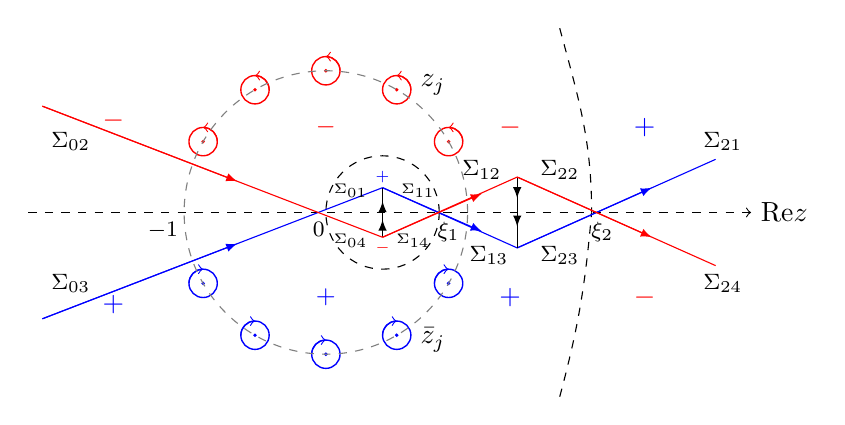
\begin{tikzpicture}[scale=0.9]
                                           %[node distance=2cm]
                               %\draw [yellow!10, fill=yellow!10] (5.6,0)--(5.6,2.6)--(3.3,2.6)--(3.7,0);
                               % \draw [yellow!10, fill=yellow!10] (-4,0)--(-4,-2.6)--(3.3,-2.6)--(3.7,0);
         \draw [dashed  ] (3.3,2.6) to [out=-75,in=90] (3.75,0);
         \draw [dashed  ] (3.3,-2.6) to [out=75,in=-95] (3.75,0);
                              %\filldraw[white](0,0)--(1.2,0) arc (0:-180:0.6);
         \draw[dashed,->](-4.2,0)--(6,0)node[black,right]{Re$z$};
         \foreach \x [count=\p] in {1,...,5} {
         \node[shape=circle,fill=red, scale=0.15] (\p) at (\x*30:2) {};
         \draw[red,line width=0.5] (\x*30:2) circle (0.2);
         \draw[red, ->] (\x*30:2)+(0.2,0) arc (0:90:0.2);
         \node[shape=circle,fill=blue, scale=0.15] (\p) at (180+\x*30:2) {};
         \draw[blue,line width=0.5] (180+\x*30:2) circle (0.2);
         \draw[blue, ->] (180+\x*30:2)+(-0.2,0) arc (180:90:0.2);
         };
                                    %   \draw[red,line width = 0.5](-1.8,0) arc(0:180:0.2);
                                    %   \draw[red,->] (-1.8,0) arc(0:90:0.2);
                                    %   \node[shape=circle,fill=black, scale=0.15] at (-2,0){};
                                   %    \draw[red,line width = 0.5](2.2,0) arc(0:180:0.2);
                                    %   \draw[red,->] (2.2,0) arc(0:90:0.2);
                                    %  \node[shape=circle,fill=black, scale=0.15] at (2,0){};
         
                                    %   \draw[blue,line width = 0.5](-2.15,0) arc(180:360:0.15);
                                   %    \draw[blue,line width = 0.5](1.85,0) arc(180:360:0.15);
         
                                      % \draw[red,line width=0.2] (\p) arc (0:360:0.2)
                                       %\foreach \x [count=\p] in {0,...,5} {
                                      %         \draw (-\x*60:2.4);
                                       %        \draw (-30-\x*60:2.4) ;};
                                         %  \node[shape=circle,fill=blue, scale=0.15]  at (0:2){0};
                                         %  \node[shape=circle,fill=blue, scale=0.15]  at (-6*30:2){0} ;
                                         %  \node[shape=circle,fill=blue,scale=0.15] at (-0.05,0) {0};
                                           %\node[below] at (2.15,0.05) {\footnotesize $1$};
         \node[below] at (-0.1,0) {\footnotesize $0$};
         \node[below] at (-2.3,0) {\footnotesize $-1$};
         \node[right] at (1.2,1.8) {$z_j$};
                                       %    \draw[red,line width=0.2] (1,1.8) arc (0:360:0.2);
         \node[right] at (1.2,-1.8) {$\bar{z}_j$};
                                       %  \node[left] at (5*30:2) {$\bar{z}_k$};
                                       %  \node[left] at (-5*30:2) {$z_k$};
         \draw [dashed, gray] (0,0) circle (2);
                                       %    \draw [dashed, gray](1) arc (0:360:2);
         \draw [dashed] (0.8,0) circle [radius=0.8];
         \draw [ blue] (-4, -1.5)--(0.8,0.35);
         \draw [ blue] (0.8,0.35 )--(2.7,-0.5);
         \draw [-latex,blue] (0.8,0.35 )--(2.2,-0.265);
         \draw [ blue] (2.7,-0.5)--(5.5, 0.75);
         \draw [-latex, blue] (2.7,-0.5)--(4.6, 0.35);
         \draw [-latex,blue] (-4, -1.5)--(-1.25,-0.44 );
         \draw[](0.8,-0.35)--(0.8,0.35);
         \draw[-latex](0.8,0)--(0.8,0.16);
         \draw[-latex](0.8,-0.35)--(0.8,-0.1);
         \draw[](2.7,-0.5)--(2.7,0.5);
         \draw[-latex](2.7,0.5)--(2.7,0.2);
         \draw[-latex](2.7,0)--(2.7,-0.2);
         \draw [ red] (0.8,-0.35)--(2.7, 0.5);
         \draw [-latex,red] (0.8,-0.35 )--(2.2,0.265);
         \draw [ red] (2.7,0.5)--(5.5, -0.75);
         \draw [ red] (-4, 1.5)--(0.8,-0.35 );
         \draw [-latex,red] (2.7, 0.5)--(4.6, -0.35);
         \draw [-latex,red] (-4,  1.5)--(-1.25, 0.44 );
         \node[blue,thick]  at (4.5,1.2) {\bf  $+$};
         \node[red,thick]  at (4.5,-1.2) {\bf  $-$};
         \node[red,thick]  at (2.6,1.2) {\bf  $-$};
         \node[blue,thick]  at (2.6,-1.2) {\bf  $+$};
         \node[red,thick]  at (0,1.2) {\small\bf $-$};
         \node[blue,thick]  at (0,-1.2) {\small\bf $+$};
         \node[blue,thick]  at (0.8,0.5) {\tiny\bf $+$};
         \node[red,thick]  at (0.8,-0.5) {\tiny\bf $-$};
         \node[blue,thick]  at (-3,-1.3) {\bf  $+$};
         \node[red,thick]  at (-3,1.3) {\bf  $-$};
         
         \node[below] at (3.9,0) {\footnotesize $\xi_2$};
         \node[below] at (1.73,0) {\footnotesize $\xi_1$};
         \node  at (5.6,1) {\footnotesize $\Sigma_{21}$};
         \node  at (5.6,-1) {\footnotesize $\Sigma_{24}$};
         \node  at (3.3,0.6) {\footnotesize $\Sigma_{22}$};
         \node  at (3.3,-0.6) {\footnotesize $\Sigma_{23}$};
         \node  at (2.2,0.6) {\footnotesize $\Sigma_{12}$};
         \node  at (2.3,-0.6) {\footnotesize $\Sigma_{13}$};
         \node  at (-3.6,1) {\footnotesize $\Sigma_{02}$};
         \node  at (-3.6,-1) {\footnotesize $\Sigma_{03}$};
         \node  at (1.3,0.3) {\tiny $\Sigma_{11}$};
         \node  at (0.35,0.3) {\tiny $\Sigma_{01}$};
         \node  at (1.23,-0.4) {\tiny $\Sigma_{14}$};
         \node  at (0.35,-0.4) {\tiny $\Sigma_{04}$};
      \end{tikzpicture}
      }%
      
      \subfigure[$ \xi<-1$]{
      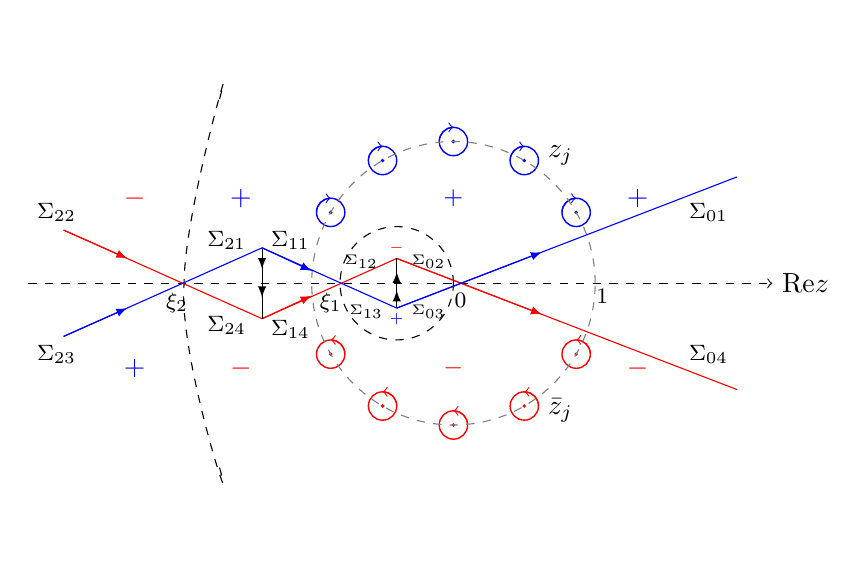
\begin{tikzpicture}[scale=0.9]
                                           %[node distance=2cm]
                               %\draw [yellow!10, fill=yellow!10] (5.6,0)--(5.6,2.6)--(3.3,2.6)--(3.7,0);
                               % \draw [yellow!10, fill=yellow!10] (-4,0)--(-4,-2.6)--(3.3,-2.6)--(3.7,0);
         \draw [dashed  ] (-3.3,2.6) to [out=75,in=90] (-3.8,0);
         \draw [dashed  ] (-3.3,-2.6) to [out=-75,in=-95] (-3.8,0);
                              %\filldraw[white](0,0)--(1.2,0) arc (0:-180:0.6);
         \draw[dashed,->](-6,0)--(4.5,0)node[black,right]{Re$z$};
         \foreach \x [count=\p] in {1,...,5} {
         \node[shape=circle,fill=blue, scale=0.15] (\p) at (\x*30:2) {};
         \draw[blue,line width=0.5] (\x*30:2) circle (0.2);
         \draw[blue, ->] (\x*30:2)+(-0.2,0) arc (180:90:0.2);
         \node[shape=circle,fill=red, scale=0.15] (\p) at (180+\x*30:2) {};
         \draw[red,line width=0.5] (180+\x*30:2) circle (0.2);
         \draw[red, ->] (180+\x*30:2)+(0.2,0) arc (0:90:0.2);
         };
         
                                       %    \foreach \x [count=\p] in {0,...,11} {
                                       %\node[shape=circle,fill=red, scale=0.25] (\p) at (-\x*30:2) {};};
                                        %   \foreach \x [count=\p] in {0,...,5} {
                                        %       \draw (-\x*60:2.4);
                                        %       \draw (-30-\x*60:2.4) ;};
                                       %    \node[shape=circle,fill=blue, scale=0.15]  at (0:2){0};
                                       %    \node[shape=circle,fill=blue, scale=0.15]  at (-6*30:2){0} ;
                                       %\node[shape=circle,fill=blue,scale=0.15] at (0.05,0) {0};
         \node[below] at (2.1,0.05) {\footnotesize $1$};
         \node[below] at (0.1,0) {\footnotesize $0$};
                                           % \node[below] at (-2.3,0) {\footnotesize $-1$};
         \node[right] at (1.2,1.8) {$z_j$};
         \node[right] at (1.2,-1.8) {$\bar{z}_j$};
                                       %  \node[left] at (5*30:2) {$\bar{z}_k$};
                                       %  \node[left] at (-5*30:2) {$z_k$};
         \draw [dashed, gray] (0,0) circle (2);
         \draw [dashed] (-0.8,0) circle [radius=0.8];
         
         \draw [ red] (4, -1.5)--(-0.8,0.35);
         \draw [ red] (-0.8,0.35 )--(-2.7,-0.5);
         \draw [-latex,red] (-2.7,-0.5)--(-2,-0.175);
         \draw [ red] (-2.7,-0.5)--(-5.5, 0.75);
         \draw [-latex, red] (-5.5, 0.75)--(-4.6, 0.35);
         \draw [-latex,red] (-0.8,0.35 )--(1.25,-0.44 );
         \draw[](-0.8,-0.35)--(-0.8,0.35);
         \draw[-latex](-0.8,0)--(-0.8,0.16);
         \draw[-latex](-0.8,-0.35)--(0-.8,-0.1);
         \draw[](-2.7,-0.5)--(-2.7,0.5);
         \draw[-latex](-2.7,0.5)--(-2.7,0.2);
         \draw[-latex](-2.7,0)--(-2.7,-0.2);
         \draw [ blue] (-0.8,-0.35)--(-2.7, 0.5);
         \draw [-latex,blue] (-2.7, 0.5)--(-2,0.175);
         \draw [blue] (-2.7,0.5)--(-5.5, -0.75);
         \draw [blue] (4, 1.5)--(-0.8,-0.35 );
         \draw [-latex,blue] (-5.5, -0.75)--(-4.6, -0.35);
         \draw [-latex,blue] (-0.8,-0.35 )--(1.25, 0.44 );
         
         \node[red,thick]  at (-4.5,1.2) {\bf  $-$};
         \node[blue,thick]  at (-4.5,-1.2) {\bf  $+$};
         \node[blue,thick]  at (2.6,1.2) {\bf  $+$};
         \node[red,thick]  at (2.6,-1.2) {\bf  $-$};
         \node[blue,thick]  at (0,1.2) {\small\bf $+$};
         \node[red,thick]  at (0,-1.2) {\small\bf $-$};
         \node[red,thick]  at (-0.8,0.5) {\tiny\bf $-$};
         \node[blue,thick]  at (-0.8,-0.5) {\tiny\bf $+$};
         \node[red,thick]  at (-3,-1.2) {\bf  $-$};
         \node[blue,thick]  at (-3,1.2) {\bf  $+$};
         
         \node[below] at (-3.9,0) {\footnotesize $\xi_2$};
         \node[below] at (-1.73,0) {\footnotesize $\xi_1$};
         \node  at (-5.6,1) {\footnotesize $\Sigma_{22}$};
         \node  at (-5.6,-1) {\footnotesize $\Sigma_{23}$};
         \node  at (-3.2,0.6) {\footnotesize $\Sigma_{21}$};
         \node  at (-3.2,-0.6) {\footnotesize $\Sigma_{24}$};
         \node  at (-2.3,0.6) {\footnotesize $\Sigma_{11}$};
         \node  at (-2.3,-0.65) {\footnotesize $\Sigma_{14}$};
         \node  at (3.6,1) {\footnotesize $\Sigma_{01}$};
         \node  at (3.6,-1) {\footnotesize $\Sigma_{04}$};
         \node  at (-1.3,0.3) {\tiny $\Sigma_{12}$};
         \node  at (-0.35,0.3) {\tiny $\Sigma_{02}$};
         \node  at (-1.23,-0.4) {\tiny $\Sigma_{13}$};
         \node  at (-0.35,-0.4) {\tiny $\Sigma_{03}$};
      \end{tikzpicture}
      }%
   \end{center}
   \caption{caption}\label{fig5}
\end{figure}



\clearpage



\begin{figure}
   \begin{center}
      \subfigure[$ \xi>1$]{
      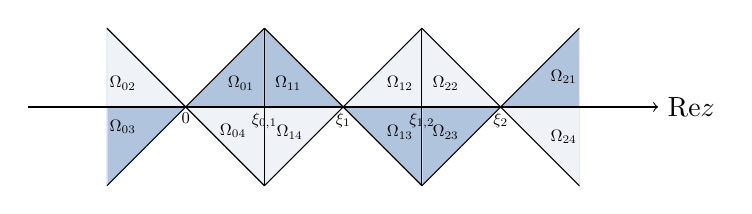
\begin{tikzpicture}
         \draw[Blue!10,fill=LightSteelBlue!] (2,0)--(3,1)--(3,0);
         \draw[Blue!10,fill=LightSteelBlue!] (2,0)--(1,-1)--(1,0);
         \draw[CadetBlue!20,fill=LightSteelBlue!20] (0,0)--(1,1)--(1,0);    
         \draw[CadetBlue!20,fill=LightSteelBlue!20] (0,0)--(-1,-1)--(-1,0);
         \draw[Blue!10,fill=LightSteelBlue!] (-2,0)--(-1,1)--(-1,0);    
         \draw[Blue!10,fill=LightSteelBlue!] (-2,0)--(-3,-1)--(-3,0);
         
         \draw[CadetBlue!20,fill=LightSteelBlue!20] (2,0)--(1,1)--(1,0);    \draw[CadetBlue!20,fill=LightSteelBlue!20] (2,0)--(3,-1)--(3,0);
         \draw[Blue!10,fill=LightSteelBlue!] (0,0)--(1,-1)--(1,0);    \draw[Blue!10,fill=LightSteelBlue!] (0,0)--(-1,1)--(-1,0);
         \draw[CadetBlue!20,fill=LightSteelBlue!20] (-2,0)--(-1,-1)--(-1,0);    \draw[CadetBlue!20,fill=LightSteelBlue!20] (-2,0)--(-3,1)--(-3,0);
         \draw[](-3.4,0)--(3.4,0);
         \draw[](0,0)--(0.5,0.5);
         \draw[](0.5,0.5)--(1,1);
         \node[below, scale=0.6] at (0,0) {$\xi_1$};
         \node[below, scale=0.6]   at (-2,0) {$0$};
         \node[below, scale=0.6]  at (2,0) {$\xi_2$};
         \node[below, scale=0.6]  at (-1,0) {$\xi_{0,1}$};
         \node[below, scale=0.6]  at (1,0) {$\xi_{1,2}$};
         \draw[](-2,0)--(-1.5,0.5);
         \draw[](-1.5,0.5)--(-1,1);
         \draw[](-3,1)--(-2.5,0.5);
         \draw[](-2.5,0.5)--(-2,0);
         \draw[](-3,-1)--(-2.5,-0.5);
         \draw[](-2.5,-0.5)--(-2,0);
         \draw[](-2,0)--(-1.5,-0.5);
         \draw[](-1.5,-0.5)--(-1,-1);    
         \draw[](-1,-1)--(-0.5,-0.5);
         \draw[](-0.5,-0.5)--(0,0);
         \draw[](0,0)--(-0.5,0.5);
         \draw[](-1,1)--(-0.5,0.5);
         \draw[](0,0)--(0.5,-0.5);
         \draw[]    (0.5,-0.5)--(1,-1);
         \draw[](1.5,0.5)--(2,0);
         \draw[](1,1)--(1.5,0.5);
         \draw[](2,0)--(1.5,-0.5);
         \draw[](1,-1)--(1.5,-0.5);
         \draw[](2,0)--(2.5,0.5);
         \draw[](3,1)--(2.5,0.5);
         \draw[](2.5,-0.5)--(3,-1);
         \draw[](2,0)--(2.5,-0.5);
         \draw[](1,0)--(1,0.5);
         \draw[](1,1)--(1,0.4);
         \draw[](1,0)--(1,-0.5);
         \draw[](1,0.5)--(1,-1);
         
         \node[scale=0.6] at (2.8,0.38) {$\Omega_{21}$};
                                    %  \node[scale=0.5] at (2.38,0.78) {$\Sigma_{21}$};
         \node[scale=0.6] at (2.8,-0.38) {$\Omega_{24}$};
                                    %  \node[scale=0.7] at (2.38,-0.78) {$\Sigma_{24}$};
         \node[scale=0.6] at (1.3,0.3) {$\Omega_{22}$};
                                    %  \node[scale=0.7] at (1.6,0.78) {$\Sigma_{22}$};
         \node[scale=0.6] at (1.3,-0.32) {$\Omega_{23}$};
                                    %  \node[scale=0.7] at (1.6,-0.78) {$\Sigma_{23}$};
         \node[scale=0.6] at (0.72,0.3) {$\Omega_{12}$};
                                    %  \node[scale=0.7] at (0.45,0.8) {$\Sigma_{12}$};
         \node[scale=0.6] at (0.72,-0.32) {$\Omega_{13}$};
                                    %  \node[scale=0.7] at (0.45,-0.8) {$\Sigma_{13}$};
         \node[scale=0.6] at (-0.7,0.3) {$\Omega_{11}$};
                                    %  \node[scale=0.7] at (-0.45,0.8) {$\Sigma_{11}$};
         \node[scale=0.6] at (-0.68,-0.32) {$\Omega_{14}$};
                                    %  \node[scale=0.7] at (-0.4,-0.8) {$\Sigma_{14}$};
         \node[scale=0.6] at (-1.3,0.3) {$\Omega_{01}$};
                                    %  \node[scale=0.7] at (-1.6,0.8) {$\Sigma_{01}$};
         \node[scale=0.6] at (-1.4,-0.3) {$\Omega_{04}$};
                                    %  \node[scale=0.7] at (-1.6,-0.8) {$\Sigma_{04}$};
         \node[scale=0.6] at (-2.8,0.3) {$\Omega_{02}$};
                                    %  \node[scale=0.7] at (-3.1,0.8) {$\Sigma_{02}$};
         \node[scale=0.6] at (-2.8,-0.25) {$\Omega_{03}$};
                                    %  \node[scale=0.7] at (-3.2,-0.8) {$\Sigma_{03}$};
         \draw[](-1,0)--(-1,0.5);
         \draw[](-1,0.5)--(-1,1);
         \draw[](-1,-1)--(-1,-0.4);
         \draw[](-1,0)--(-1,-0.5);
         \draw[ ->](-4,0)--(4,0)node[black,right]{Re$z$};
      \end{tikzpicture}
      }%
      
      \subfigure[$ \xi<-1$]{
      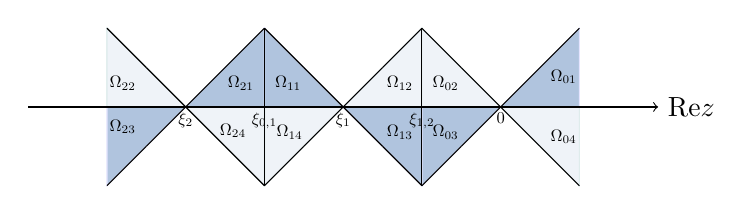
\begin{tikzpicture}
         \draw[Blue!10,fill=LightSteelBlue!] (2,0)--(3,1)--(3,0);
         \draw[Blue!10,fill=LightSteelBlue!] (2,0)--(1,-1)--(1,0);
         \draw[CadetBlue!20,fill=LightSteelBlue!20] (0,0)--(1,1)--(1,0);    
         \draw[CadetBlue!20,fill=LightSteelBlue!20] (0,0)--(-1,-1)--(-1,0);
         \draw[Blue!10,fill=LightSteelBlue!] (-2,0)--(-1,1)--(-1,0);    
         \draw[Blue!10,fill=LightSteelBlue!] (-2,0)--(-3,-1)--(-3,0);
         
         \draw[CadetBlue!20,fill=LightSteelBlue!20] (2,0)--(1,1)--(1,0);    \draw[CadetBlue!20,fill=LightSteelBlue!20] (2,0)--(3,-1)--(3,0);
         \draw[Blue!10,fill=LightSteelBlue!] (0,0)--(1,-1)--(1,0);    \draw[Blue!10,fill=LightSteelBlue!] (0,0)--(-1,1)--(-1,0);
         \draw[CadetBlue!20,fill=LightSteelBlue!20] (-2,0)--(-1,-1)--(-1,0);    \draw[CadetBlue!20,fill=LightSteelBlue!20] (-2,0)--(-3,1)--(-3,0);    \draw[CadetBlue!20,fill=LightSteelBlue!20] (-2,0)--(-3,1)--(-3,0);
         \draw[](-3.4,0)--(3.4,0);
         \draw[](0,0)--(0.5,0.5);
         \draw[](0.5,0.5)--(1,1);
         \node[below, scale=0.6] at (0,0) {$\xi_1$};
         \node[below, scale=0.6]   at (-2,0) {$\xi_2$};
         \node[below, scale=0.6]  at (2,0) {$0$};
         \node[below, scale=0.6]  at (-1,0) {$\xi_{0,1}$};
         \node[below, scale=0.6]  at (1,0) {$\xi_{1,2}$};
         \draw[](-2,0)--(-1.5,0.5);
         \draw[](-1.5,0.5)--(-1,1);
         \draw[](-3,1)--(-2.5,0.5);
         \draw[](-2.5,0.5)--(-2,0);
         \draw[](-3,-1)--(-2.5,-0.5);
         \draw[](-2.5,-0.5)--(-2,0);
         \draw[](-2,0)--(-1.5,-0.5);
         \draw[](-1.5,-0.5)--(-1,-1);    
         \draw[](-1,-1)--(-0.5,-0.5);
         \draw[](-0.5,-0.5)--(0,0);
         \draw[](0,0)--(-0.5,0.5);
         \draw[](-1,1)--(-0.5,0.5);
         \draw[](0,0)--(0.5,-0.5);
         \draw[]    (0.5,-0.5)--(1,-1);
         \draw[](1.5,0.5)--(2,0);
         \draw[](1,1)--(1.5,0.5);
         \draw[](2,0)--(1.5,-0.5);
         \draw[](1,-1)--(1.5,-0.5);
         \draw[](2,0)--(2.5,0.5);
         \draw[](3,1)--(2.5,0.5);
         \draw[](2.5,-0.5)--(3,-1);
         \draw[](2,0)--(2.5,-0.5);
         \draw[](1,0)--(1,0.5);
         \draw[](1,1)--(1,0.4);
         \draw[](1,0)--(1,-0.5);
         \draw[](1,0.5)--(1,-1);
         
         \node[scale=0.6] at (2.8,0.38) {$\Omega_{01}$};
                                    %  \node[scale=0.5] at (2.38,0.78) {$\Sigma_{21}$};
         \node[scale=0.6] at (2.8,-0.38) {$\Omega_{04}$};
                                    %  \node[scale=0.7] at (2.38,-0.78) {$\Sigma_{24}$};
         \node[scale=0.6] at (1.3,0.3) {$\Omega_{02}$};
                                    %  \node[scale=0.7] at (1.6,0.78) {$\Sigma_{22}$};
         \node[scale=0.6] at (1.3,-0.32) {$\Omega_{03}$};
                                    %  \node[scale=0.7] at (1.6,-0.78) {$\Sigma_{23}$};
         \node[scale=0.6] at (0.72,0.3) {$\Omega_{12}$};
                                    %  \node[scale=0.7] at (0.45,0.8) {$\Sigma_{12}$};
         \node[scale=0.6] at (0.72,-0.32) {$\Omega_{13}$};
                                    %  \node[scale=0.7] at (0.45,-0.8) {$\Sigma_{13}$};
         \node[scale=0.6] at (-0.7,0.3) {$\Omega_{11}$};
                                    %  \node[scale=0.7] at (-0.45,0.8) {$\Sigma_{11}$};
         \node[scale=0.6] at (-0.68,-0.32) {$\Omega_{14}$};
                                    %  \node[scale=0.7] at (-0.4,-0.8) {$\Sigma_{14}$};
         \node[scale=0.6] at (-1.3,0.3) {$\Omega_{21}$};
                                    %  \node[scale=0.7] at (-1.6,0.8) {$\Sigma_{01}$};
         \node[scale=0.6] at (-1.4,-0.3) {$\Omega_{24}$};
                                    %  \node[scale=0.7] at (-1.6,-0.8) {$\Sigma_{04}$};
         \node[scale=0.6] at (-2.8,0.3) {$\Omega_{22}$};
                                    %  \node[scale=0.7] at (-3.1,0.8) {$\Sigma_{02}$};
         \node[scale=0.6] at (-2.8,-0.25) {$\Omega_{23}$};
                                    %  \node[scale=0.7] at (-3.2,-0.8) {$\Sigma_{03}$};
         \draw[](-1,0)--(-1,0.5);
         \draw[](-1,0.5)--(-1,1);
         \draw[](-1,-1)--(-1,-0.4);
         \draw[](-1,0)--(-1,-0.5);
         \draw[](-1,0)--(-1,-0.5);
         \draw[ ->](-4,0)--(4,0)node[black,right]{Re$z$};
      \end{tikzpicture}
      }%
   \end{center}
   \caption{caption}\label{rj1}
\end{figure}



\clearpage



\begin{figure}
   \begin{center}
      \subfigure[\footnotesize\ \ $ \xi>1$]{
      \begin{tikzpicture}
         \draw(-1,0)--(-0.4,0.3);
         \draw[->](-1,0)--(-0.6,0.2);
         \draw(-1,0)--(-1.6,0.3);
         \draw[-<](-1,0)--(-1.4,-0.2);
         \draw(-1,0)--(-0.4,-0.3);
         \draw[-<](-1,0)--(-1.4,0.2);
         \draw(-1,0)--(-1.6,-0.3);
         \draw[->](-1,0)--(-0.6,-0.2);
         \draw[dashed,blue](-1,0) circle (0.65);
         \node at    ( 2,0.9) {\footnotesize $ \mathcal{U}_{\xi_2}$};
         \node at    (-1,0.9) {\footnotesize $ \mathcal{U}_{\xi_1}$};
         \draw[->,dashed](-4,0)--(4,0)node[right]{ \textcolor{black}{Re$z$}};
         \draw[->,dashed](-2.3,-1.5)--(-2.3,1.5)node[right]{\textcolor{black}{Im$z$}};
         \draw(2,0)--(1.4,0.3);
         \draw[-<](2,0)--(1.6,0.2);
         \draw(2,0)--(1.4,-0.3);
         \draw[->](2,0)--(2.4,-0.2);
         \draw(2,0)--(2.6,0.3);
         \draw[->](2,0)--(2.4,0.2);
         \draw(2,0)--(2.6,-0.3);
         \draw[-<](2,0)--(1.6,-0.2);
         \draw[dashed,blue](2,0) circle (0.65);
         \coordinate (I) at (0,0);
         \fill[red] (I) circle (1pt) node[below] {$1$};
         \coordinate (b) at (-1,0);
         \fill (b) circle (1pt) node[blue,below] {$\xi_1$};
         \coordinate (f) at (2,0);
         \fill (f) circle (1pt) node[blue,below] {$\xi_2$};
         \node[shape=circle,fill=red,scale=0.11] at (-2.3,0) {0};
         \node[below,red] at (-2.5,0) {$0$};
      \end{tikzpicture}
      \label{si1}}\\
      \subfigure[\footnotesize \ \ $ \xi<-1$]{
      \begin{tikzpicture}
         \draw(-1,0)--(-0.4,0.3);
         \draw[->](-1,0)--(-0.6,0.2);
         \draw(-1,0)--(-1.6,0.3);
         \draw[-<](-1,0)--(-1.4,-0.2);
         \draw(-1,0)--(-0.4,-0.3);
         \draw[-<](-1,0)--(-1.4,0.2);
         \draw(-1,0)--(-1.6,-0.3);
         \draw[->](-1,0)--(-.6,-0.2);
         
         \draw[->,dashed](-4,0)--(4,0)node[right]{ \textcolor{black}{Re$z$}};
         \draw[->,dashed,black](3.3,-1.5)--(3.3,1.5)node[right]{\textcolor{black}{Im$z$}};
         
         \draw(2,0)--(1.4,0.3);
         \draw[-<](2,0)--(1.6,0.2);
         \draw(2,0)--(2.6,-0.3);
         \draw[->](2,0)--(2.4,-0.2);
         \draw(2,0)--(2.6,0.3);
         \draw[->](2,0)--(2.4,0.2);
         \draw(2,0)--(1.4,-0.3);
         \draw[-<](2,0)--(1.6,-0.2);
         \coordinate (I) at (1,0);
         \fill[red] (I) circle (1pt) node[below] {$-1$};
                           %  \coordinate (A) at (-4,0);
                           %     \fill (A) circle (1pt) node[blue,below] {$\xi_4$};
         \coordinate (b) at (-1,0);
         \fill (b) circle (1pt) node[blue,below] {$\xi_2$};
                           %     \coordinate (e) at (4,0);
                           %  \fill (e) circle (1pt) node[blue,below] {$\xi_1$};
         \coordinate (f) at (2,0);
         \fill (f) circle (1pt) node[blue,below] {$\xi_1$};
                           %  \coordinate (c) at (2,0);
                           %  \fill[red] (c) circle (1pt) node[below] {$0$};
         \node[shape=circle,fill=red,scale=0.11] at (3.3,0) {0};
         \node[below,red] at (3.5,0) {$0$};
         \draw[dashed,blue](2,0) circle (0.65);
         \draw[dashed,blue](-1,0) circle (0.65);
      \end{tikzpicture}
      \label{si2}}
      \caption{caption}\label{local}
   \end{center}
\end{figure}



\clearpage



\begin{figure}
   \begin{center}
      \subfigure[The \ region $ \xi>1$]{
      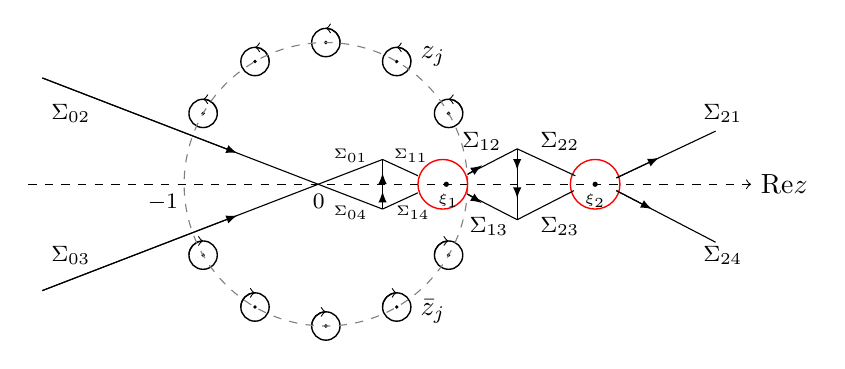
\begin{tikzpicture}[scale=0.9]
                           %\draw [dashed  ] (3.3,2.6) to [out=-75,in=90] (3.75,0);
                           %\draw [dashed  ] (3.3,-2.6) to [out=75,in=-95] (3.75,0);
         \draw[dashed,->](-4.2,0)--(6,0)node[black,right]{Re$z$};
         \foreach \x [count=\p] in {1,...,5} {
         \node[shape=circle,fill=black, scale=0.15] (\p) at (\x*30:2) {};
         \draw[line width=0.5] (\x*30:2) circle (0.2);
         \draw[ ->] (\x*30:2)+(0.2,0) arc (0:90:0.2);
         \node[shape=circle,fill=black, scale=0.15] (\p) at (180+\x*30:2) {};
         \draw[line width=0.5] (180+\x*30:2) circle (0.2);
         \draw[ ->] (180+\x*30:2)+(-0.2,0) arc (180:90:0.2);
         };
         
         \node[below] at (-0.1,0) {\footnotesize $0$};
         \node[below] at (-2.3,0) {\footnotesize $-1$};
         \node[right] at (1.2,1.8) {$z_j$};
         \node[right] at (1.2,-1.8) {$\bar{z}_j$};
         
         \draw [dashed, gray] (0,0) circle (2);
         \draw [red,line width=0.5] (1.65,0) circle (0.35);
         \node[shape=circle,fill=black, scale=0.2]  at (1.7,0) {};
         \node[below] at (1.73,0) {\tiny $\xi_1$};
         
         \draw [red,line width=0.5] (3.8,0) circle (0.35);
         \node[shape=circle,fill=black, scale=0.2]  at (3.8,0) {};
         \node[below] at (3.8,0) {\tiny $\xi_2$};
         
         \draw  (-4, -1.5)--(0.8,0.35);
         \draw  (2,-0.14 )--(2.7,-0.5);
         \draw  (0.8,0.35 )--(1.3,0.12);
         \draw [-latex] (2,-0.14 )--(2.2,-0.265);
         \draw  (2.7,-0.5)--(3.5, -0.09);
         \draw (2.7,0.5)--(3.52, 0.12);
         \draw  (4.1,0.09)--(5.5, 0.75);
         \draw [-latex]  (4.1,0.09)--(4.7, 0.373);
                                               %\draw [-latex] (2.7,-0.5)--(4.6, 0.35);
         
         \draw (0.8,-0.35)--(1.3, -0.12);
         \draw [-latex] (2,0.14 )--(2.2,0.265);
         \draw  (2,0.14 )--(2.7,0.5);
         \draw (4.1,-0.09)--(5.5, -0.818);
         \draw [-latex] (4.1, -0.09)--(4.6, -0.35);
         
         \draw [-latex] (-4, -1.5)--(-1.25,-0.44 );
         \draw[](0.8,-0.35)--(0.8,0.35);
         \draw[-latex](0.8,0)--(0.8,0.16);
         \draw[-latex](0.8,-0.35)--(0.8,-0.1);
         \draw[](2.7,-0.5)--(2.7,0.5);
         \draw[-latex](2.7,0.5)--(2.7,0.2);
         \draw[-latex](2.7,0)--(2.7,-0.2);
         
         \draw (-4, 1.5)--(0.8,-0.35 );
         \draw [-latex] (-4,  1.5)--(-1.25, 0.44 );
                                                        % \node[blue,thick]  at (4.5,1.2) {\bf  $+$};
                                                        %    \node[red,thick]  at (4.5,-1.2) {\bf  $-$};
                                                        %      \node[red,thick]  at (2.6,1.2) {\bf  $-$};
                                                        %    \node[blue,thick]  at (2.6,-1.2) {\bf  $+$};
                                                        %    \node[red,thick]  at (0,1.2) {\small\bf $-$};
                                                        %    \node[blue,thick]  at (0,-1.2) {\small\bf $+$};
                                                        %     \node[blue,thick]  at (0.8,0.5) {\tiny\bf $+$};
                                                        %        \node[red,thick]  at (0.8,-0.5) {\tiny\bf $-$};
                                                        %        \node[blue,thick]  at (-3,-1.3) {\bf  $+$};
                                                        %        \node[red,thick]  at (-3,1.3) {\bf  $-$};
         
         \node  at (5.6,1) {\footnotesize $\Sigma_{21}$};
         \node  at (5.6,-1) {\footnotesize $\Sigma_{24}$};
         \node  at (3.3,0.6) {\footnotesize $\Sigma_{22}$};
         \node  at (3.3,-0.6) {\footnotesize $\Sigma_{23}$};
         \node  at (2.2,0.6) {\footnotesize $\Sigma_{12}$};
         \node  at (2.3,-0.6) {\footnotesize $\Sigma_{13}$};
         \node  at (-3.6,1) {\footnotesize $\Sigma_{02}$};
         \node  at (-3.6,-1) {\footnotesize $\Sigma_{03}$};
         
         \node  at (1.2,0.4) {\tiny $\Sigma_{11}$};
         \node  at (0.35,0.4) {\tiny $\Sigma_{01}$};
         \node  at (1.23,-0.4) {\tiny $\Sigma_{14}$};
         \node  at (0.35,-0.4) {\tiny $\Sigma_{04}$};
      \end{tikzpicture}
      }%
      
      \subfigure[The \ region  $ \xi<-1$]{
      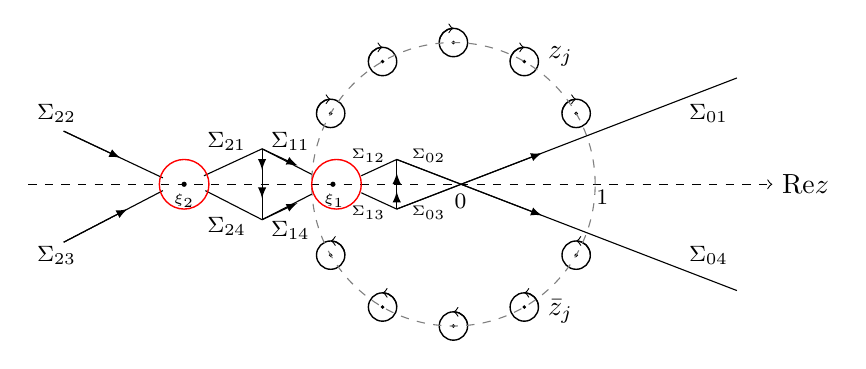
\begin{tikzpicture}[scale=0.9]
                           %\draw [dashed  ] (-3.3,2.6) to [out=75,in=90] (-3.8,0);
                           %\draw [dashed  ] (-3.3,-2.6) to [out=-75,in=-95] (-3.8,0);
         
         \draw[dashed,->](-6,0)--(4.5,0)node[black,right]{Re$z$};
         \foreach \x [count=\p] in {1,...,5} {
         \node[shape=circle,fill=black, scale=0.15] (\p) at (\x*30:2) {};
         \draw[line width=0.5] (\x*30:2) circle (0.2);
         \draw[ ->] (\x*30:2)+(-0.2,0) arc (180:90:0.2);
         \node[shape=circle,fill=black, scale=0.15] (\p) at (180+\x*30:2) {};
         \draw[line width=0.5] (180+\x*30:2) circle (0.2);
         \draw[ ->] (180+\x*30:2)+(0.2,0) arc (0:90:0.2);
         };
         
         \node[below] at (2.1,0.05) {\footnotesize $1$};
         \node[below] at (0.1,0) {\footnotesize $0$};
         \node[right] at (1.2,1.8) {$z_j$};
         \node[right] at (1.2,-1.8) {$\bar{z}_j$};
         \draw [dashed, gray] (0,0) circle (2);
                           %           \draw [dashed] (-0.8,0) circle [radius=0.8];
         
                           %                             \draw [ red] (4, -1.5)--(-0.8,0.35);
                           %                             \draw [ red] (-0.8,0.35 )--(-2.7,-0.5);
                           %                             \draw [-latex,red] (-2.7,-0.5)--(-2,-0.175);
                           %                       \draw [ red] (-2.7,-0.5)--(-5.5, 0.75);
                           %                       \draw [-latex, red] (-5.5, 0.75)--(-4.6, 0.35);
                           %\draw [-latex,red] (-0.8,0.35 )--(1.25,-0.44 );
                           %\draw[](-0.8,-0.35)--(-0.8,0.35);
                           %\draw[->](-0.8,0)--(-0.8,0.16);
                           %\draw[->](-0.8,-0.35)--(0-.8,-0.1);
                           %\draw[](-2.7,-0.5)--(-2.7,0.5);
                           %\draw[->](-2.7,0.5)--(-2.7,0.2);
                           %\draw[->](-2.7,0)--(-2.7,-0.2);
                           %                         \draw [ blue] (-0.8,-0.35)--(-2.7, 0.5);
                           %                            \draw [-latex,blue] (-2.7, 0.5)--(-2,0.175);
                           %                            \draw [blue] (-2.7,0.5)--(-5.5, -0.75);
                           %                            \draw [blue] (4, 1.5)--(-0.8,-0.35 );
                           %                             \draw [-latex,blue] (-5.5, -0.75)--(-4.6, -0.35);
                           %                               \draw [-latex,blue] (-0.8,-0.35 )--(1.25, 0.44 );
         
         \draw  (4, -1.5)--(-0.8,0.35);
         \draw[-latex] (-0.8,0.35)--(1.25,-0.44 );
         
         \draw (4, 1.5)--(-0.8,-0.35 );
         \draw [-latex] (-0.8,-0.35 )--(1.25, 0.44 );
         
         \draw  (-4.1,0.09)--(-5.5, 0.75);
         \draw [-latex]  (-5.5, 0.75)--(-4.7, 0.373);
         
         \draw (-4.1,-0.09)--(-5.5, -0.818);
         \draw [-latex] (-5.5, -0.818)--(-4.6, -0.35);
         
         \draw  (-2,-0.14 )--(-2.7,-0.5);
         \draw [-latex] (-2.7,-0.5)--(-2.2,-0.265);
         \draw  (-0.8,0.35 )--(-1.3,0.12);
         
         \draw  (-2.7,-0.5)--(-3.5, -0.09);
         \draw (-2.7,0.5)--(-3.52, 0.12);
         \draw (-0.8,-0.35)--(-1.3, -0.12);
         \draw [-latex] (-2.7,0.5)--(-2.2,0.265);
         
         \draw  (-2,0.14 )--(-2.7,0.5);
         
         \draw[](-0.8,-0.35)--(-0.8,0.35);
         \draw[-latex](-0.8,0)--(-0.8,0.16);
         \draw[-latex](-0.8,-0.35)--(-0.8,-0.1);
         \draw[](-2.7,-0.5)--(-2.7,0.5);
         \draw[-latex](-2.7,0.5)--(-2.7,0.2);
         \draw[-latex](-2.7,0)--(-2.7,-0.2);
         
                                                     %    \node[red,thick]  at (-4.5,1.2) {\bf  $-$};
                                                    %        \node[blue,thick]  at (-4.5,-1.2) {\bf  $+$};
                                                      %        \node[blue,thick]  at (2.6,1.2) {\bf  $+$};
                                                     %       \node[red,thick]  at (2.6,-1.2) {\bf  $-$};
                                                     %       \node[blue,thick]  at (0,1.2) {\small\bf $+$};
                                                     %       \node[red,thick]  at (0,-1.2) {\small\bf $-$};
                                                     %        \node[red,thick]  at (-0.8,0.5) {\tiny\bf $-$};
                                                    %            \node[blue,thick]  at (-0.8,-0.5) {\tiny\bf $+$};
                                                     %           \node[red,thick]  at (-3,-1.2) {\bf  $-$};
                                                     %           \node[blue,thick]  at (-3,1.2) {\bf  $+$};
         
         \draw [red,line width=0.5] (-1.65,0) circle (0.35);
         \node[shape=circle,fill=black, scale=0.2]  at (-1.7,0) {};
         \node[below] at (-1.68,0) {\tiny $\xi_1$};
         
         \draw [red,line width=0.5] (-3.8,0) circle (0.35);
         \node[shape=circle,fill=black, scale=0.2]  at (-3.8,0) {};
         \node[below] at (-3.8,0) {\tiny $\xi_2$};
         
                                                           %     \node[below] at (-3.9,0) {\footnotesize $\xi_2$};
                                                           %     \node[below] at (-1.73,0) {\footnotesize $\xi_1$};
         \node  at (-5.6,1) {\footnotesize $\Sigma_{22}$};
         \node  at (-5.6,-1) {\footnotesize $\Sigma_{23}$};
         \node  at (-3.2,0.6) {\footnotesize $\Sigma_{21}$};
         \node  at (-3.2,-0.6) {\footnotesize $\Sigma_{24}$};
         \node  at (-2.3,0.6) {\footnotesize $\Sigma_{11}$};
         \node  at (-2.3,-0.65) {\footnotesize $\Sigma_{14}$};
         \node  at (3.6,1) {\footnotesize $\Sigma_{01}$};
         \node  at (3.6,-1) {\footnotesize $\Sigma_{04}$};
         \node  at (-1.2,0.4) {\tiny $\Sigma_{12}$};
         \node  at (-0.35,0.4) {\tiny $\Sigma_{02}$};
         \node  at (-1.2,-0.4) {\tiny $\Sigma_{13}$};
         \node  at (-0.35,-0.4) {\tiny $\Sigma_{03}$};
      \end{tikzpicture}
      }%
   \end{center}
   \caption{caption}\label{figE}
\end{figure}



\clearpage



\begin{figure}
   \centering
   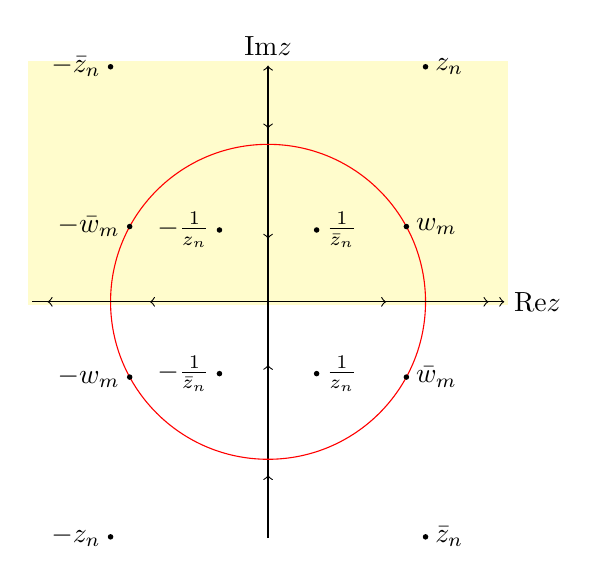
\begin{tikzpicture}[node distance=2cm]
      \filldraw[yellow!20,line width=3] (3,0.01) rectangle (0.01,3);
      \filldraw[yellow!20,line width=3] (-3,0.01) rectangle (-0.01,3);
      \draw[->](-3,0)--(3,0)node[right]{Re$z$};
      \draw[->](0,-3)--(0,3)node[above]{Im$z$};
      \draw[red] (2,0) arc (0:360:2);
      \draw[->](0,0)--(-1.5,0);
      \draw[->](-1.5,0)--(-2.8,0);
      \draw[->](0,0)--(1.5,0);
      \draw[->](1.5,0)--(2.8,0);
      \draw[->](0,2.7)--(0,2.2);
      \draw[->](0,1.6)--(0,0.8);
      \draw[->](0,-2.7)--(0,-2.2);
      \draw[->](0,-1.6)--(0,-0.8);
      \coordinate (A) at (2,2.985);
      \coordinate (B) at (2,-2.985);
      \coordinate (C) at (-0.616996232,0.9120505887);
      \coordinate (D) at (-0.616996232,-0.9120505887);
      \coordinate (E) at (0.616996232,0.9120505887);
      \coordinate (F) at (0.616996232,-0.9120505887);
      \coordinate (G) at (-2,2.985);
      \coordinate (H) at (-2,-2.985);
      \coordinate (J) at (1.7570508075688774,0.956);
      \coordinate (K) at (1.7570508075688774,-0.956);
      \coordinate (L) at (-1.7570508075688774,0.956);
      \coordinate (M) at (-1.7570508075688774,-0.956);
      \fill (A) circle (1pt) node[right] {$z_n$};
      \fill (B) circle (1pt) node[right] {$\bar{z}_n$};
      \fill (C) circle (1pt) node[left] {$-\frac{1}{z_n}$};
      \fill (D) circle (1pt) node[left] {$-\frac{1}{\bar{z}_n}$};
      \fill (E) circle (1pt) node[right] {$\frac{1}{\bar{z}_n}$};
      \fill (F) circle (1pt) node[right] {$\frac{1}{z_n}$};
      \fill (G) circle (1pt) node[left] {$-\bar{z}_n$};
      \fill (H) circle (1pt) node[left] {$-z_n$};
      \fill (J) circle (1pt) node[right] {$w_m$};
      \fill (K) circle (1pt) node[right] {$\bar{w}_m$};
      \fill (L) circle (1pt) node[left] {$-\bar{w}_m$};
      \fill (M) circle (1pt) node[left] {$-w_m$};
   \end{tikzpicture}
   \caption{caption}\label{fig:figure1}
\end{figure}



\clearpage



\begin{figure}
   \subfigure[]{
   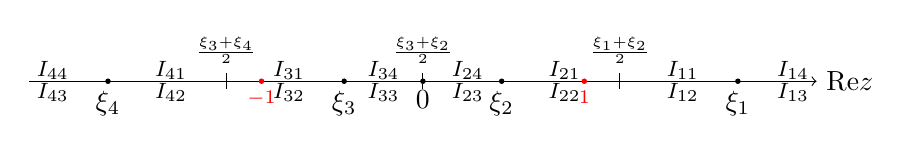
\begin{tikzpicture}
      \draw[->](-5,0)--(5,0)node[right]{ Re$z$};
      \draw(2.5,0)--(2.5,0.1)node[above]{\scriptsize$\frac{\xi_1+\xi_2}{2}$};
      \draw(2.5,0)--(2.5,-0.1);
      \draw(-2.5,0)--(-2.5,0.1)node[above]{\scriptsize$\frac{\xi_3+\xi_4}{2}$};
      \draw(-2.5,0)--(-2.5,-0.1);
      \draw(0,0)--(0,0.1)node[above]{\scriptsize$\frac{\xi_3+\xi_2}{2}$};
      \draw(0,0)--(0,-0.1);
      \coordinate (I) at (0,0);
      \fill (I) circle (1pt) node[below] {$0$};
      \coordinate (A) at (-4,0);
      \fill (A) circle (1pt) node[below] {$\xi_4$};
      \coordinate (b) at (-1,0);
      \fill (b) circle (1pt) node[below] {$\xi_3$};
      \coordinate (e) at (4,0);
      \fill (e) circle (1pt) node[below] {$\xi_1$};
      \coordinate (f) at (1,0);
      \fill (f) circle (1pt) node[below] {$\xi_2$};
      \coordinate (ke) at (4.7,0.1);
      \fill (ke) circle (0pt) node[below] {\footnotesize$I_{13}$};
      \coordinate (k1e) at (4.7,-0.1);
      \fill (k1e) circle (0pt) node[above] {\footnotesize$I_{14}$};
      \coordinate (le) at (3.3,0.1);
      \fill (le) circle (0pt) node[below] {\footnotesize$I_{12}$};
      \coordinate (l1e) at (3.3,-0.1);
      \fill (l1e) circle (0pt) node[above] {\footnotesize$I_{11}$};
      \coordinate (n2) at (0.57,0.1);
      \fill (n2) circle (0pt) node[below] {\footnotesize$I_{23}$};
      \coordinate (n12) at (0.57,-0.1);
      \fill (n12) circle (0pt) node[above] {\footnotesize$I_{24}$};
      \coordinate (m2) at (1.8,0.1);
      \fill (m2) circle (0pt) node[below] {\footnotesize$I_{22}$};
      \coordinate (m12) at (1.8,-0.1);
      \fill (m12) circle (0pt) node[above] {\footnotesize$I_{21}$};
      \coordinate (k) at (-4.7,0.1);
      \fill (k) circle (0pt) node[below] {\footnotesize$I_{43}$};
      \coordinate (k1) at (-4.7,-0.1);
      \fill (k1) circle (0pt) node[above] {\footnotesize$I_{44}$};
      \coordinate (l) at (-3.2,0.1);
      \fill (l) circle (0pt) node[below] {\footnotesize$I_{42}$};
      \coordinate (l1) at (-3.2,-0.1);
      \fill (l1) circle (0pt) node[above] {\footnotesize$I_{41}$};
      \coordinate (n) at (-0.5,0.1);
      \fill (n) circle (0pt) node[below] {\footnotesize$I_{33}$};
      \coordinate (n1) at (-0.5,-0.1);
      \fill (n1) circle (0pt) node[above] {\footnotesize$I_{34}$};
      \coordinate (m) at (-1.7,0.1);
      \fill (m) circle (0pt) node[below] {\footnotesize$I_{32}$};
      \coordinate (m1) at (-1.7,-0.1);
      \fill (m1) circle (0pt) node[above] {\footnotesize$I_{31}$};
      \coordinate (c) at (-2.05,0);
      \fill[red] (c) circle (1pt) node[below] {\scriptsize$-1$};
      \coordinate (d) at (2.05,0);
      \fill[red] (d) circle (1pt) node[below] {\scriptsize$1$};
   \end{tikzpicture}
   \label{pcase1}}
   \subfigure[]{
   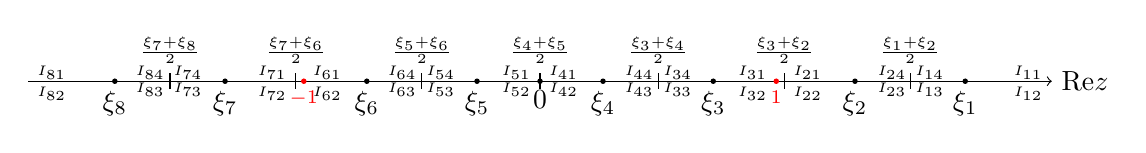
\begin{tikzpicture}
      \draw[->](-6.5,0)--(6.5,0)node[right]{ Re$z$};
      \coordinate (I) at (0,0);
      \fill (I) circle (1pt) node[below] {$0$};
      \coordinate (c) at (-3,0);
      \fill[red] (c) circle (1pt) node[below] {\scriptsize$-1$};
      \coordinate (D) at (3,0);
      \fill[red] (D) circle (1pt) node[below] {\scriptsize$1$};
      \draw(-1.5,0)--(-1.5,0.1)node[above]{\scriptsize$\frac{\xi_5+\xi_6}{2}$};
      \draw(-1.5,0)--(-1.5,-0.1);
      \draw(-4.7,0)--(-4.7,0.1)node[above]{\scriptsize$\frac{\xi_7+\xi_8}{2}$};
      \draw(-4.7,0)--(-4.7,-0.1);
      \draw(-3.1,0)--(-3.1,0.1)node[above]{\scriptsize$\frac{\xi_7+\xi_6}{2}$};
      \draw(-3.1,0)--(-3.1,-0.1);
      \draw(1.5,0)--(1.5,0.1)node[above]{\scriptsize$\frac{\xi_3+\xi_4}{2}$};
      \draw(1.5,0)--(1.5,-0.1);
      \draw(4.7,0)--(4.7,0.1)node[above]{\scriptsize$\frac{\xi_1+\xi_2}{2}$};
      \draw(4.7,0)--(4.7,-0.1);
      \draw(3.1,0)--(3.1,0.1)node[above]{\scriptsize$\frac{\xi_3+\xi_2}{2}$};
      \draw(3.1,0)--(3.1,-0.1);
      \draw(0,0)--(0,0.1)node[above]{\scriptsize$\frac{\xi_4+\xi_5}{2}$};
      \draw(0,0)--(0,-0.1);
      \coordinate (A) at (-5.4,0);
      \fill (A) circle (1pt) node[below] {$\xi_8$};
      \coordinate (b) at (-4,0);
      \fill (b) circle (1pt) node[below] {$\xi_7$};
      \coordinate (C) at (-0.8,0);
      \fill (C) circle (1pt) node[below] {$\xi_5$};
      \coordinate (d) at (-2.2,0);
      \fill (d) circle (1pt) node[below] {$\xi_6$};
      \coordinate (E) at (5.4,0);
      \fill (E) circle (1pt) node[below] {$\xi_1$};
      \coordinate (R) at (4,0);
      \fill (R) circle (1pt) node[below] {$\xi_2$};
      \coordinate (T) at (0.8,0);
      \fill (T) circle (1pt) node[below] {$\xi_4$};
      \coordinate (Y) at (2.2,0);
      \fill (Y) circle (1pt) node[below] {$\xi_3$};
      \coordinate (q) at (6.2,-0.1);
      \fill (q) circle (0pt) node[above] {\tiny$I_{11}$};
      \coordinate (q1) at (6.2,0.05);
      \fill (q1) circle (0pt) node[below] {\tiny$I_{12}$};
      \coordinate (w) at (4.95,-0.1);
      \fill (w) circle (0pt) node[above] {\tiny$I_{14}$};
      \coordinate (w1) at (4.95,0.1);
      \fill (w1) circle (0pt) node[below] {\tiny$I_{13}$};
      \coordinate (e) at (4.47,-0.1);
      \fill (e) circle (0pt) node[above] {\tiny$I_{24}$};
      \coordinate (e1) at (4.47,0.1);
      \fill (e1) circle (0pt) node[below] {\tiny$I_{23}$};
      \coordinate (r) at (3.4,-0.1);
      \fill (r) circle (0pt) node[above] {\tiny$I_{21}$};
      \coordinate (r1) at (3.4,0.05);
      \fill (r1) circle (0pt) node[below] {\tiny$I_{22}$};
      \coordinate (t) at (2.7,-0.1);
      \fill (t) circle (0pt) node[above] {\tiny$I_{31}$};
      \coordinate (t1) at (2.7,0.05);
      \fill (t1) circle (0pt) node[below] {\tiny$I_{32}$};
      \coordinate (y) at (1.75,-0.1);
      \fill (y) circle (0pt) node[above] {\tiny$I_{34}$};
      \coordinate (y1) at (1.75,0.1);
      \fill (y1) circle (0pt) node[below] {\tiny$I_{33}$};
      \coordinate (l) at (1.26,-0.1);
      \fill (l) circle (0pt) node[above] {\tiny$I_{44}$};
      \coordinate (l1) at (1.26,0.1);
      \fill (l1) circle (0pt) node[below] {\tiny$I_{43}$};
      \coordinate (k) at (0.3,-0.1);
      \fill (k) circle (0pt) node[above] {\tiny$I_{41}$};
      \coordinate (k1) at (0.3,0.1);
      \fill (k1) circle (0pt) node[below] {\tiny$I_{42}$};
      \coordinate (q8) at (-6.2,-0.1);
      \fill (q8) circle (0pt) node[above] {\tiny$I_{81}$};
      \coordinate (q18) at (-6.2,0.05);
      \fill (q18) circle (0pt) node[below] {\tiny$I_{82}$};
      \coordinate (w8) at (-4.95,-0.1);
      \fill (w8) circle (0pt) node[above] {\tiny$I_{84}$};
      \coordinate (w18) at (-4.95,0.1);
      \fill (w18) circle (0pt) node[below] {\tiny$I_{83}$};
      \coordinate (e7) at (-4.47,-0.1);
      \fill (e7) circle (0pt) node[above] {\tiny$I_{74}$};
      \coordinate (e17) at (-4.47,0.1);
      \fill (e17) circle (0pt) node[below] {\tiny$I_{73}$};
      \coordinate (7r) at (-3.4,-0.1);
      \fill (7r) circle (0pt) node[above] {\tiny$I_{71}$};
      \coordinate (r17) at (-3.4,0.05);
      \fill (r17) circle (0pt) node[below] {\tiny$I_{72}$};
      \coordinate (t6) at (-2.7,-0.1);
      \fill (t6) circle (0pt) node[above] {\tiny$I_{61}$};
      \coordinate (t16) at (-2.7,0.05);
      \fill (t16) circle (0pt) node[below] {\tiny$I_{62}$};
      \coordinate (y6) at (-1.75,-0.1);
      \fill (y6) circle (0pt) node[above] {\tiny$I_{64}$};
      \coordinate (y16) at (-1.75,0.1);
      \fill (y16) circle (0pt) node[below] {\tiny$I_{63}$};
      \coordinate (l5) at (-1.26,-0.1);
      \fill (l5) circle (0pt) node[above] {\tiny$I_{54}$};
      \coordinate (l15) at (-1.26,0.1);
      \fill (l15) circle (0pt) node[below] {\tiny$I_{53}$};
      \coordinate (k5) at (-0.3,-0.1);
      \fill (k5) circle (0pt) node[above] {\tiny$I_{51}$};
      \coordinate (k15) at (-0.3,0.1);
      \fill (k15) circle (0pt) node[below] {\tiny$I_{52}$};
   \end{tikzpicture}
   \label{phase2}}
   \caption{caption}\label{phase}
\end{figure}



\clearpage



\begin{figure}
   \subfigure[]{
   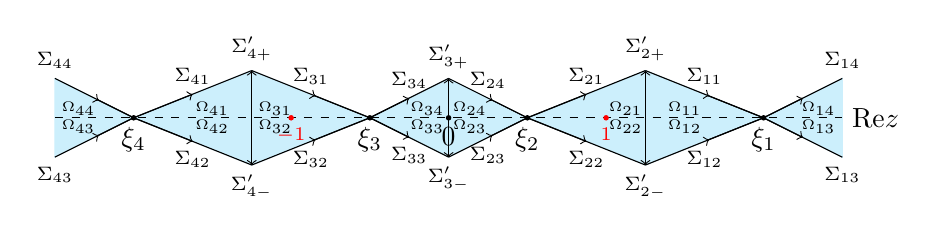
\begin{tikzpicture}
      \draw[cyan!20, fill=cyan!20] (-5,0.5)--(-5,-0.5)--(-4,0)--(-2.5,-0.6)--(-1,0)--(0,-0.5)--(1,0)--(2.5,-0.6)--(4,0)--(5,-0.5)--(5,0.5)--(4,0)--(2.5,0.6)--(1,0)--(0,0.5)--(-1,0)--(-2.5,0.6)--(-4,0)--(-5,0.5);
      \draw(-4,0)--(-5,0.5)node[above]{\scriptsize$\Sigma_{44}$};
      \draw[-<](-4,0)--(-4.5,0.25);
      \draw(-4,0)--(-2.5,0.6);
      \draw[->](-4,0)--(-3.25,-0.3)node[below]{\scriptsize$\Sigma_{42}$};
      \draw(-4,0)--(-5,-0.5)node[below]{\scriptsize$\Sigma_{43}$};
      \draw[->](-4,0)--(-3.25,0.3)node[above]{\scriptsize$\Sigma_{41}$};
      \draw(-4,0)--(-2.5,-0.6);
      \draw[-<](-4,0)--(-4.5,-0.25);
      \draw(-1,0)--(0,0.5);
      \draw[->](-1,0)--(-0.5,0.25)node[above]{\scriptsize$\Sigma_{34}$};
      \draw(-1,0)--(-2.5,0.6);
      \draw[-<](-1,0)--(-1.75,-0.3)node[below]{\scriptsize$\Sigma_{32}$};
      \draw(-1,0)--(0,-0.5);
      \draw[-<](-1,0)--(-1.75,0.3)node[above]{\scriptsize$\Sigma_{31}$};
      \draw(-1,0)--(-2.5,-0.6);
      \draw[->](-1,0)--(-0.5,-0.25)node[below]{\scriptsize$\Sigma_{33}$};
      \draw[dashed](-5,0)--(5,0)node[right]{ Re$z$};
      \draw(1,0)--(0,0.5);
      \draw[-<](1,0)--(0.5,0.25)node[above]{\scriptsize$\Sigma_{24}$};
      \draw(1,0)--(2.5,0.6);
      \draw[->](1,0)--(1.75,-0.3)node[below]{\scriptsize$\Sigma_{22}$};
      \draw(1,0)--(0,-0.5);
      \draw[->](1,0)--(1.75,0.3)node[above]{\scriptsize$\Sigma_{21}$};
      \draw(1,0)--(2.5,-0.6);
      \draw[-<](1,0)--(0.5,-0.25)node[below]{\scriptsize$\Sigma_{23}$};
      \draw(4,0)--(5,0.5)node[above]{\scriptsize$\Sigma_{14}$};
      \draw[->](4,0)--(4.5,0.25);
      \draw(4,0)--(2.5,0.6);
      \draw[-<](4,0)--(3.25,-0.3)node[below]{\scriptsize$\Sigma_{12}$};
      \draw(4,0)--(5,-0.5)node[below]{\scriptsize$\Sigma_{13}$};
      \draw[-<](4,0)--(3.25,0.3)node[above]{\scriptsize$\Sigma_{11}$};
      \draw(4,0)--(2.5,-0.6);
      \draw[->](4,0)--(4.5,-0.25);
      \draw[->](2.5,0)--(2.5,0.6)node[above]{\scriptsize$\Sigma_{2+}'$};
      \draw[->](2.5,0)--(2.5,-0.6)node[below]{\scriptsize$\Sigma_{2-}'$};
      \draw[->](-2.5,0)--(-2.5,0.6)node[above]{\scriptsize$\Sigma_{4+}'$};
      \draw[->](-2.5,0)--(-2.5,-0.6)node[below]{\scriptsize$\Sigma_{4-}'$};
      \draw[->](0,0)--(0,0.5)node[above]{\scriptsize$\Sigma_{3+}'$};
      \draw[->](0,0)--(0,-0.5)node[below]{\scriptsize$\Sigma_{3-}'$};
      \coordinate (I) at (0,0);
      \fill (I) circle (1pt) node[below] {$0$};
      \coordinate (A) at (-4,0);
      \fill (A) circle (1pt) node[below] {$\xi_4$};
      \coordinate (b) at (-1,0);
      \fill (b) circle (1pt) node[below] {$\xi_3$};
      \coordinate (e) at (4,0);
      \fill (e) circle (1pt) node[below] {$\xi_1$};
      \coordinate (f) at (1,0);
      \fill (f) circle (1pt) node[below] {$\xi_2$};
      \coordinate (ke) at (4.7,0.1);
      \fill (ke) circle (0pt) node[below] {\tiny$\Omega_{13}$};
      \coordinate (k1e) at (4.7,-0.1);
      \fill (k1e) circle (0pt) node[above] {\tiny$\Omega_{14}$};
      \coordinate (le) at (3,0.1);
      \fill (le) circle (0pt) node[below] {\tiny$\Omega_{12}$};
      \coordinate (l1e) at (3,-0.1);
      \fill (l1e) circle (0pt) node[above] {\tiny$\Omega_{11}$};
      \coordinate (n2) at (0.27,0.1);
      \fill (n2) circle (0pt) node[below] {\tiny$\Omega_{23}$};
      \coordinate (n12) at (0.27,-0.1);
      \fill (n12) circle (0pt) node[above] {\tiny$\Omega_{24}$};
      \coordinate (m2) at (2.25,0.1);
      \fill (m2) circle (0pt) node[below] {\tiny$\Omega_{22}$};
      \coordinate (m12) at (2.25,-0.1);
      \fill (m12) circle (0pt) node[above] {\tiny$\Omega_{21}$};
      \coordinate (k) at (-4.7,0.1);
      \fill (k) circle (0pt) node[below] {\tiny$\Omega_{43}$};
      \coordinate (k1) at (-4.7,-0.1);
      \fill (k1) circle (0pt) node[above] {\tiny$\Omega_{44}$};
      \coordinate (l) at (-3,0.1);
      \fill (l) circle (0pt) node[below] {\tiny$\Omega_{42}$};
      \coordinate (l1) at (-3,-0.1);
      \fill (l1) circle (0pt) node[above] {\tiny$\Omega_{41}$};
      \coordinate (n) at (-0.27,0.1);
      \fill (n) circle (0pt) node[below] {\tiny$\Omega_{33}$};
      \coordinate (n1) at (-0.27,-0.1);
      \fill (n1) circle (0pt) node[above] {\tiny$\Omega_{34}$};
      \coordinate (m) at (-2.2,0.1);
      \fill (m) circle (0pt) node[below] {\tiny$\Omega_{32}$};
      \coordinate (m1) at (-2.2,-0.1);
      \fill (m1) circle (0pt) node[above] {\tiny$\Omega_{31}$};
      \coordinate (c) at (-2,0);
      \fill[red] (c) circle (1pt) node[below] {\scriptsize$-1$};
      \coordinate (d) at (2,0);
      \fill[red] (d) circle (1pt) node[below] {\scriptsize$1$};
   \end{tikzpicture}
   \label{case1}}
   \subfigure[]{
   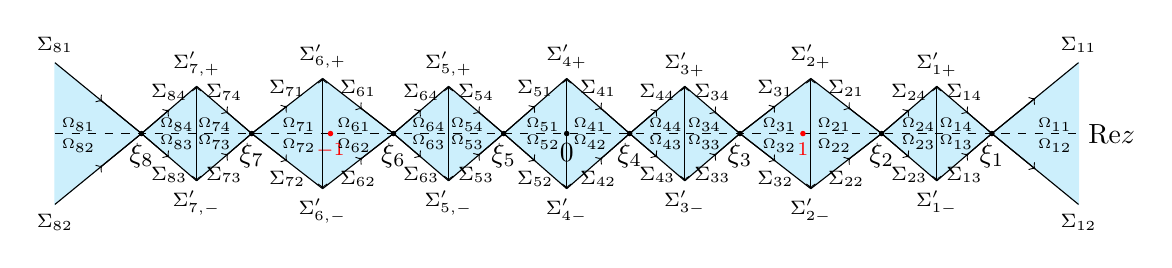
\begin{tikzpicture}
      \draw[cyan!20, fill=cyan!20](-6.5,0.9)--(-6.5,-0.9)--(-5.4,0)--(-4.7,-0.6)--(-4,0)--(-3.1,-0.7)--(-2.2,0)--(-1.5,-0.6)--(-0.8,0)
      --(-0,-0.7)--(0.8,0)--(1.5,-0.6)--(2.2,0)--(3.1,-0.7)--(4,0)--(4.7,-0.6)--(5.4,0)--(6.5,-0.9)--(6.5,0.9)--(5.4,0)--(4.7,0.6)
      --(4,0)--(3.1,0.7)--(2.2,0)--(1.5,0.6)--(0.8,0)--(-0,0.7)--(-0.8,0)--(-1.5,0.6)--(-2.2,0)--(-3.1,0.7)--(-4,0)--(-4.7,0.6)--(-5.4,0)--(-6.5,0.9);
      \draw[dashed](-6.5,0)--(6.5,0)node[right]{ Re$z$};
      \coordinate (I) at (0,0);
      \fill (I) circle (1pt) node[below] {$0$};
      \coordinate (c) at (-3,0);
      \fill[red] (c) circle (1pt) node[below] {\scriptsize$-1$};
      \coordinate (D) at (3,0);
      \fill[red] (D) circle (1pt) node[below] {\scriptsize$1$};
      \draw(-0.8,0)--(-0,0.7);
      \draw[->](-0.8,0)--(-0.4,0.35)node[above]{\scriptsize$\Sigma_{51}$};
      \draw(-0.8,0)--(-1.5,0.6);
      \draw[-<](-0.8,0)--(-1.15,-0.3)node[below]{\scriptsize$\Sigma_{53}$};
      \draw(-0.8,0)--(-0,-0.7);
      \draw[-<](-0.8,0)--(-1.15,0.3)node[above]{\scriptsize$\Sigma_{54}$};
      \draw(-0.8,0)--(-1.5,-0.6);
      \draw[->](-0.8,0)--(-0.4,-0.35)node[below]{\scriptsize$\Sigma_{52}$};
      \draw(-2.2,0)--(-1.5,0.6);
      \draw[-<](-2.2,0)--(-2.65,0.35)node[above]{\scriptsize$\Sigma_{61}$};
      \draw(-2.2,0)--(-1.5,-0.6);
      \draw[->](-2.2,0)--(-1.85,-0.3)node[below]{\scriptsize$\Sigma_{63}$};
      \draw(-2.2,0)--(-3.1,0.7);
      \draw[->](-2.2,0)--(-1.85,0.3)node[above]{\scriptsize$\Sigma_{64}$};
      \draw(-2.2,0)--(-3.1,-0.7);
      \draw[-<](-2.2,0)--(-2.65,-0.35)node[below]{\scriptsize$\Sigma_{62}$};
      \draw(-5.4,0)--(-6.5,0.9)node[above]{\scriptsize$\Sigma_{81}$};
      \draw[-<](-5.4,0)--(-5.95,0.45);
      \draw(-5.4,0)--(-4.7,0.6);
      \draw[->](-5.4,0)--(-5.05,-0.3)node[below]{\scriptsize$\Sigma_{83}$};
      \draw(-5.4,0)--(-6.5,-0.9)node[below]{\scriptsize$\Sigma_{82}$};
      \draw[->](-5.4,0)--(-5.05,0.3)node[above]{\scriptsize$\Sigma_{84}$};
      \draw(-5.4,0)--(-4.7,-0.6);
      \draw[-<](-5.4,0)--(-5.95,-0.45);
      \draw(-4,0)--(-3.1,0.7);
      \draw[->](-4,0)--(-3.55,0.35)node[above]{\scriptsize$\Sigma_{71}$};
      \draw(-4,0)--(-4.7,0.6);
      \draw[-<](-4,0)--(-4.35,-0.3)node[below]{\scriptsize$\Sigma_{73}$};
      \draw(-4,0)--(-3.1,-0.7);
      \draw[-<](-4,0)--(-4.35,0.3)node[above]{\scriptsize$\Sigma_{74}$};
      \draw(-4,0)--(-4.7,-0.6);
      \draw[->](-4,0)--(-3.55,-0.35)node[below]{\scriptsize$\Sigma_{72}$};
      \draw[->](-1.5,0)--(-1.5,0.6)node[above]{\scriptsize$\Sigma_{5,+}'$};
      \draw[->](-1.5,0)--(-1.5,-0.6)node[below]{\scriptsize$\Sigma_{5,-}'$};
      \draw[->](-4.7,0)--(-4.7,0.6)node[above]{\scriptsize$\Sigma_{7,+}'$};
      \draw[->](-4.7,0)--(-4.7,-0.6)node[below]{\scriptsize$\Sigma_{7,-}'$};
      \draw[->](-3.1,0)--(-3.1,0.7)node[above]{\scriptsize$\Sigma_{6,+}'$};
      \draw[->](-3.1,0)--(-3.1,-0.7)node[below]{\scriptsize$\Sigma_{6,-}'$};
      \draw(0.8,0)--(0,0.7);
      \draw[-<](0.8,0)--(0.4,0.35)node[above]{\scriptsize$\Sigma_{41}$};
      \draw(0.8,0)--(1.5,0.6);
      \draw[->](0.8,0)--(1.15,-0.3)node[below]{\scriptsize$\Sigma_{43}$};
      \draw(0.8,0)--(0,-0.7);
      \draw[->](0.8,0)--(1.15,0.3)node[above]{\scriptsize$\Sigma_{44}$};
      \draw(0.8,0)--(1.5,-0.6);
      \draw[-<](0.8,0)--(0.4,-0.35)node[below]{\scriptsize$\Sigma_{42}$};
      \draw(2.2,0)--(1.5,0.6);
      \draw[->](2.2,0)--(2.65,0.35)node[above]{\scriptsize$\Sigma_{31}$};
      \draw(2.2,0)--(1.5,-0.6);
      \draw[-<](2.2,0)--(1.85,-0.3)node[below]{\scriptsize$\Sigma_{33}$};
      \draw(2.2,0)--(3.1,0.7);
      \draw[-<](2.2,0)--(1.85,0.3)node[above]{\scriptsize$\Sigma_{34}$};
      \draw(2.2,0)--(3.1,-0.7);
      \draw[->](2.2,0)--(2.65,-0.35)node[below]{\scriptsize$\Sigma_{32}$};
      \draw(5.4,0)--(6.5,0.9)node[above]{\scriptsize$\Sigma_{11}$};
      \draw[->](5.4,0)--(5.95,0.45);
      \draw(5.4,0)--(4.7,0.6);
      \draw[-<](5.4,0)--(5.05,-0.3)node[below]{\scriptsize$\Sigma_{13}$};
      \draw(5.4,0)--(6.5,-0.9)node[below]{\scriptsize$\Sigma_{12}$};
      \draw[-<](5.4,0)--(5.05,0.3)node[above]{\scriptsize$\Sigma_{14}$};
      \draw(5.4,0)--(4.7,-0.6);
      \draw[->](5.4,0)--(5.95,-0.45);
      \draw(4,0)--(3.1,0.7);
      \draw[-<](4,0)--(3.55,0.35)node[above]{\scriptsize$\Sigma_{21}$};
      \draw(4,0)--(4.7,0.6);
      \draw[->](4,0)--(4.35,-0.3)node[below]{\scriptsize$\Sigma_{23}$};
      \draw(4,0)--(3.1,-0.7);
      \draw[->](4,0)--(4.35,0.3)node[above]{\scriptsize$\Sigma_{24}$};
      \draw(4,0)--(4.7,-0.6);
      \draw[-<](4,0)--(3.55,-0.35)node[below]{\scriptsize$\Sigma_{22}$};
      \draw[->](1.5,0)--(1.5,0.6)node[above]{\scriptsize$\Sigma_{3+}'$};
      \draw[->](1.5,0)--(1.5,-0.6)node[below]{\scriptsize$\Sigma_{3-}'$};
      \draw[->](4.7,0)--(4.7,0.6)node[above]{\scriptsize$\Sigma_{1+}'$};
      \draw[->](4.7,0)--(4.7,-0.6)node[below]{\scriptsize$\Sigma_{1-}'$};
      \draw[->](3.1,0)--(3.1,0.7)node[above]{\scriptsize$\Sigma_{2+}'$};
      \draw[->](3.1,0)--(3.1,-0.7)node[below]{\scriptsize$\Sigma_{2-}'$};
      \draw[->](0,0)--(0,0.7)node[above]{\scriptsize$\Sigma_{4+}'$};
      \draw[->](0,0)--(0,-0.7)node[below]{\scriptsize$\Sigma_{4-}'$};
      \coordinate (A) at (-5.4,0);
      \fill (A) circle (1pt) node[below] {$\xi_8$};
      \coordinate (b) at (-4,0);
      \fill (b) circle (1pt) node[below] {$\xi_7$};
      \coordinate (C) at (-0.8,0);
      \fill (C) circle (1pt) node[below] {$\xi_5$};
      \coordinate (d) at (-2.2,0);
      \fill (d) circle (1pt) node[below] {$\xi_6$};
      \coordinate (E) at (5.4,0);
      \fill (E) circle (1pt) node[below] {$\xi_1$};
      \coordinate (R) at (4,0);
      \fill (R) circle (1pt) node[below] {$\xi_2$};
      \coordinate (T) at (0.8,0);
      \fill (T) circle (1pt) node[below] {$\xi_4$};
      \coordinate (Y) at (2.2,0);
      \fill (Y) circle (1pt) node[below] {$\xi_3$};
      \coordinate (q) at (6.2,-0.1);
      \fill (q) circle (0pt) node[above] {\tiny$\Omega_{11}$};
      \coordinate (q1) at (6.2,0.05);
      \fill (q1) circle (0pt) node[below] {\tiny$\Omega_{12}$};
      \coordinate (w) at (4.95,-0.1);
      \fill (w) circle (0pt) node[above] {\tiny$\Omega_{14}$};
      \coordinate (w1) at (4.95,0.1);
      \fill (w1) circle (0pt) node[below] {\tiny$\Omega_{13}$};
      \coordinate (e) at (4.47,-0.1);
      \fill (e) circle (0pt) node[above] {\tiny$\Omega_{24}$};
      \coordinate (e1) at (4.47,0.1);
      \fill (e1) circle (0pt) node[below] {\tiny$\Omega_{23}$};
      \coordinate (r) at (3.4,-0.1);
      \fill (r) circle (0pt) node[above] {\tiny$\Omega_{21}$};
      \coordinate (r1) at (3.4,0.05);
      \fill (r1) circle (0pt) node[below] {\tiny$\Omega_{22}$};
      \coordinate (t) at (2.7,-0.1);
      \fill (t) circle (0pt) node[above] {\tiny$\Omega_{31}$};
      \coordinate (t1) at (2.7,0.05);
      \fill (t1) circle (0pt) node[below] {\tiny$\Omega_{32}$};
      \coordinate (y) at (1.75,-0.1);
      \fill (y) circle (0pt) node[above] {\tiny$\Omega_{34}$};
      \coordinate (y1) at (1.75,0.1);
      \fill (y1) circle (0pt) node[below] {\tiny$\Omega_{33}$};
      \coordinate (l) at (1.26,-0.1);
      \fill (l) circle (0pt) node[above] {\tiny$\Omega_{44}$};
      \coordinate (l1) at (1.26,0.1);
      \fill (l1) circle (0pt) node[below] {\tiny$\Omega_{43}$};
      \coordinate (k) at (0.3,-0.1);
      \fill (k) circle (0pt) node[above] {\tiny$\Omega_{41}$};
      \coordinate (k1) at (0.3,0.1);
      \fill (k1) circle (0pt) node[below] {\tiny$\Omega_{42}$};
      \coordinate (q8) at (-6.2,-0.1);
      \fill (q8) circle (0pt) node[above] {\tiny$\Omega_{81}$};
      \coordinate (q18) at (-6.2,0.05);
      \fill (q18) circle (0pt) node[below] {\tiny$\Omega_{82}$};
      \coordinate (w8) at (-4.95,-0.1);
      \fill (w8) circle (0pt) node[above] {\tiny$\Omega_{84}$};
      \coordinate (w18) at (-4.95,0.1);
      \fill (w18) circle (0pt) node[below] {\tiny$\Omega_{83}$};
      \coordinate (e7) at (-4.47,-0.1);
      \fill (e7) circle (0pt) node[above] {\tiny$\Omega_{74}$};
      \coordinate (e17) at (-4.47,0.1);
      \fill (e17) circle (0pt) node[below] {\tiny$\Omega_{73}$};
      \coordinate (7r) at (-3.4,-0.1);
      \fill (7r) circle (0pt) node[above] {\tiny$\Omega_{71}$};
      \coordinate (r17) at (-3.4,0.05);
      \fill (r17) circle (0pt) node[below] {\tiny$\Omega_{72}$};
      \coordinate (t6) at (-2.7,-0.1);
      \fill (t6) circle (0pt) node[above] {\tiny$\Omega_{61}$};
      \coordinate (t16) at (-2.7,0.05);
      \fill (t16) circle (0pt) node[below] {\tiny$\Omega_{62}$};
      \coordinate (y6) at (-1.75,-0.1);
      \fill (y6) circle (0pt) node[above] {\tiny$\Omega_{64}$};
      \coordinate (y16) at (-1.75,0.1);
      \fill (y16) circle (0pt) node[below] {\tiny$\Omega_{63}$};
      \coordinate (l5) at (-1.26,-0.1);
      \fill (l5) circle (0pt) node[above] {\tiny$\Omega_{54}$};
      \coordinate (l15) at (-1.26,0.1);
      \fill (l15) circle (0pt) node[below] {\tiny$\Omega_{53}$};
      \coordinate (k5) at (-0.3,-0.1);
      \fill (k5) circle (0pt) node[above] {\tiny$\Omega_{51}$};
      \coordinate (k15) at (-0.3,0.1);
      \fill (k15) circle (0pt) node[below] {\tiny$\Omega_{52}$};
   \end{tikzpicture}
   \label{case2}}
   \caption{caption}\label{FigOmig}
\end{figure}



\clearpage



\begin{figure}
   \centering
   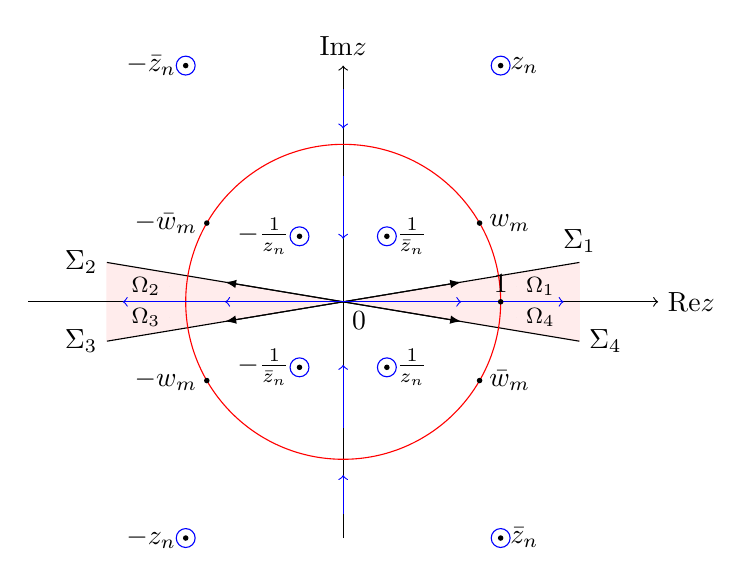
\begin{tikzpicture}[node distance=2cm]
      \draw[pink!30, fill=pink!30] (0,0)--(3,-0.5)--(3,0.5)--(0,0)--(-3,-0.5)--(-3,0.5)--(0,0);
      \draw(0,0)--(3,0.5)node[above]{$\Sigma_1$};
      \draw(0,0)--(-3,0.5)node[left]{$\Sigma_2$};
      \draw(0,0)--(-3,-0.5)node[left]{$\Sigma_3$};
      \draw(0,0)--(3,-0.5)node[right]{$\Sigma_4$};
      \draw[->](-4,0)--(4,0)node[right]{ Re$z$};
      \draw[->](0,-3)--(0,3)node[above]{ Im$z$};
      \draw[-latex](0,0)--(-1.5,-0.25);
      \draw[-latex](0,0)--(-1.5,0.25);
      \draw[-latex](0,0)--(1.5,0.25);
      \draw[-latex](0,0)--(1.5,-0.25);
      \coordinate (C) at (-0.2,2.2);
      \coordinate (D) at (2.2,0.2);
      \fill (D) circle (0pt) node[right] {\footnotesize $\Omega_1$};
      \coordinate (J) at (-2.2,-0.2);
      \fill (J) circle (0pt) node[left] {\footnotesize $\Omega_3$};
      \coordinate (k) at (-2.2,0.2);
      \fill (k) circle (0pt) node[left] {\footnotesize $\Omega_2$};
      \coordinate (k) at (2.2,-0.2);
      \fill (k) circle (0pt) node[right] {\footnotesize $\Omega_4$};
      \coordinate (I) at (0.2,0);
      \fill (I) circle (0pt) node[below] {$0$};
      \draw[red] (2,0) arc (0:360:2);
      \draw[blue] (2,3) circle (0.12);
      \draw[blue][->](0,0)--(-1.5,0);
      \draw[blue][->](-1.5,0)--(-2.8,0);
      \draw[blue][->](0,0)--(1.5,0);
      \draw[blue][->](1.5,0)--(2.8,0);
      \draw[blue][->](0,2.7)--(0,2.2);
      \draw[blue][->](0,1.6)--(0,0.8);
      \draw[blue][->](0,-2.7)--(0,-2.2);
      \draw[blue][->](0,-1.6)--(0,-0.8);
      \coordinate (A) at (2,3);
      \coordinate (B) at (2,-3);
      \coordinate (C) at (-0.5546996232,0.8320505887);
      \coordinate (D) at (-0.5546996232,-0.8320505887);
      \coordinate (E) at (0.5546996232,0.8320505887);
      \coordinate (F) at (0.5546996232,-0.8320505887);
      \coordinate (G) at (-2,3);
      \coordinate (H) at (-2,-3);
      \coordinate (I) at (2,0);
      \draw[blue] (2,-3) circle (0.12);
      \draw[blue] (-0.55469962326,0.8320505887) circle (0.12);
      \draw[blue] (0.5546996232,0.8320505887) circle (0.12);
      \draw[blue] (-0.5546996232,-0.8320505887) circle (0.12);
      \draw[blue] (0.5546996232,-0.8320505887) circle (0.12);
      \draw[blue] (-2,3) circle (0.12);
      \draw[blue] (-2,-3) circle (0.12);
      \coordinate (J) at (1.7320508075688774,1);
      \coordinate (K) at (1.7320508075688774,-1);
      \coordinate (L) at (-1.7320508075688774,1);
      \coordinate (M) at (-1.7320508075688774,-1);
      \fill (A) circle (1pt) node[right] {$z_n$};
      \fill (B) circle (1pt) node[right] {$\bar{z}_n$};
      \fill (C) circle (1pt) node[left] {$-\frac{1}{z_n}$};
      \fill (D) circle (1pt) node[left] {$-\frac{1}{\bar{z}_n}$};
      \fill (E) circle (1pt) node[right] {$\frac{1}{\bar{z}_n}$};
      \fill (F) circle (1pt) node[right] {$\frac{1}{z_n}$};
      \fill (G) circle (1pt) node[left] {$-\bar{z}_n$};
      \fill (H) circle (1pt) node[left] {$-z_n$};
      \fill (I) circle (1pt) node[above] {$1$};
      \fill (J) circle (1pt) node[right] {$w_m$};
      \fill (K) circle (1pt) node[right] {$\bar{w}_m$};
      \fill (L) circle (1pt) node[left] {$-\bar{w}_m$};
      \fill (M) circle (1pt) node[left] {$-w_m$};
   \end{tikzpicture}
   \caption{caption}\label{figR2}
\end{figure}



\clearpage



\begin{figure}
   \subfigure[]{
   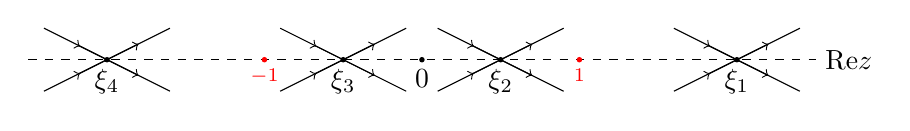
\begin{tikzpicture}
      \draw(-4,0)--(-4.8,0.4);
      \draw[-<](-4,0)--(-4.4,0.2);
      \draw(-4,0)--(-3.2,0.4);
      \draw[->](-4,0)--(-3.6,-0.2);
      \draw(-4,0)--(-4.8,-0.4);
      \draw[->](-4,0)--(-3.6,0.2);
      \draw(-4,0)--(-3.2,-0.4);
      \draw[-<](-4,0)--(-4.4,-0.2);
      \draw(-1,0)--(-0.2,0.4);
      \draw[->](-1,0)--(-0.6,0.2);
      \draw(-1,0)--(-1.8,0.4);
      \draw[-<](-1,0)--(-1.4,-0.2);
      \draw(-1,0)--(-0.2,-0.4);
      \draw[-<](-1,0)--(-1.4,0.2);
      \draw(-1,0)--(-1.8,-0.4);
      \draw[->](-1,0)--(-0.6,-0.2);
      \draw[dashed](-5,0)--(5,0)node[right]{ Re$z$};
      \draw(1,0)--(0.2,0.4);
      \draw[-<](1,0)--(0.6,0.2);
      \draw(1,0)--(0.2,-0.4);
      \draw[->](1,0)--(1.4,-0.2);
      \draw(1,0)--(1.8,0.4);
      \draw[->](1,0)--(1.4,0.2);
      \draw(1,0)--(1.8,-0.4);
      \draw[-<](1,0)--(0.6,-0.2);
      \draw(4,0)--(4.8,0.4);
      \draw[->](4,0)--(4.4,0.2);
      \draw(4,0)--(3.2,0.4);
      \draw[-<](4,0)--(3.6,-0.2);
      \draw(4,0)--(4.8,-0.4);
      \draw[-<](4,0)--(3.6,0.2);
      \draw(4,0)--(3.2,-0.4);
      \draw[->](4,0)--(4.4,-0.2);
      \coordinate (I) at (0,0);
      \fill (I) circle (1pt) node[below] {$0$};
      \coordinate (A) at (-4,0);
      \fill (A) circle (1pt) node[below] {$\xi_4$};
      \coordinate (b) at (-1,0);
      \fill (b) circle (1pt) node[below] {$\xi_3$};
      \coordinate (e) at (4,0);
      \fill (e) circle (1pt) node[below] {$\xi_1$};
      \coordinate (f) at (1,0);
      \fill (f) circle (1pt) node[below] {$\xi_2$};
      \coordinate (c) at (-2,0);
      \fill[red] (c) circle (1pt) node[below] {\scriptsize$-1$};
      \coordinate (d) at (2,0);
      \fill[red] (d) circle (1pt) node[below] {\scriptsize$1$};
   \end{tikzpicture}
   \label{si1}}
   \subfigure[]{
   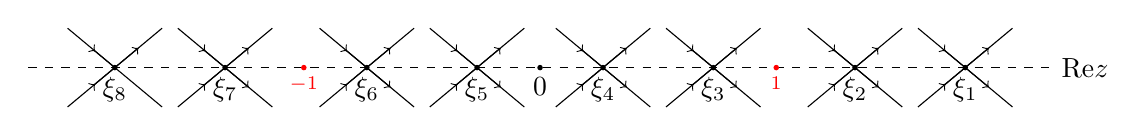
\begin{tikzpicture}
      \draw[dashed](-6.5,0)--(6.5,0)node[right]{ Re$z$};
      \coordinate (I) at (0,0);
      \fill (I) circle (1pt) node[below] {$0$};
      \coordinate (c) at (-3,0);
      \fill[red] (c) circle (1pt) node[below] {\scriptsize$-1$};
      \coordinate (D) at (3,0);
      \fill[red] (D) circle (1pt) node[below] {\scriptsize$1$};
      \draw(-0.8,0)--(-0.2,0.5);
      \draw[->](-0.8,0)--(-0.5,0.25);
      \draw(-0.8,0)--(-1.4,0.5);
      \draw[-<](-0.8,0)--(-1.1,-0.25);
      \draw(-0.8,0)--(-0.2,-0.5);
      \draw[-<](-0.8,0)--(-1.1,0.25);
      \draw(-0.8,0)--(-1.4,-0.5);
      \draw[->](-0.8,0)--(-0.5,-0.25);
      \draw(-2.2,0)--(-1.6,0.5);
      \draw[-<](-2.2,0)--(-2.5,0.25);
      \draw(-2.2,0)--(-1.6,-0.5);
      \draw[->](-2.2,0)--(-1.9,-0.25);
      \draw(-2.2,0)--(-2.8,0.5);
      \draw[->](-2.2,0)--(-1.9,0.25);
      \draw(-2.2,0)--(-2.8,-0.5);
      \draw[-<](-2.2,0)--(-2.5,-0.25);
      \draw(-5.4,0)--(-6,0.5);
      \draw[-<](-5.4,0)--(-5.7,0.25);
      \draw(-5.4,0)--(-4.8,0.5);
      \draw(-5.4,0)--(-6,-0.5);
      \draw[->](-5.4,0)--(-5.1,0.25);
      \draw(-5.4,0)--(-4.8,-0.5);
      \draw[-<](-5.4,0)--(-5.7,-0.25);
      \draw(-4,0)--(-3.4,0.5);
      \draw[->](-4,0)--(-3.7,0.25);
      \draw(-4,0)--(-4.6,0.5);
      \draw[-<](-4,0)--(-4.3,-0.25);
      \draw(-4,0)--(-3.4,-0.5);
      \draw[-<](-4,0)--(-4.3,0.25);
      \draw(-4,0)--(-4.6,-0.5);
      \draw[->](-4,0)--(-3.7,-0.25);
      \draw(0.8,0)--(0.2,0.5);
      \draw[-<](0.8,0)--(0.5,0.25);
      \draw(0.8,0)--(1.4,0.5);
      \draw[->](0.8,0)--(1.1,-0.25);
      \draw(0.8,0)--(0.2,-0.5);
      \draw[->](0.8,0)--(1.1,0.25);
      \draw(0.8,0)--(1.4,-0.5);
      \draw[-<](0.8,0)--(0.5,-0.25);
      \draw(2.2,0)--(1.6,0.5);
      \draw[->](2.2,0)--(2.5,0.25);
      \draw(2.2,0)--(1.6,-0.5);
      \draw[-<](2.2,0)--(1.9,-0.25);
      \draw(2.2,0)--(2.8,0.5);
      \draw[-<](2.2,0)--(1.9,0.25);
      \draw(2.2,0)--(2.8,-0.5);
      \draw[->](2.2,0)--(2.5,-0.25);
      \draw(5.4,0)--(6,0.5);
      \draw[->](5.4,0)--(5.7,0.25);
      \draw(5.4,0)--(4.8,0.5);
      \draw[-<](5.4,0)--(5.1,-0.25);
      \draw(5.4,0)--(6,-0.5);
      \draw[-<](5.4,0)--(5.1,0.25);
      \draw(5.4,0)--(4.8,-0.5);
      \draw[->](5.4,0)--(5.7,-0.25);
      \draw(4,0)--(3.4,0.5);
      \draw[-<](4,0)--(3.7,0.25);
      \draw(4,0)--(4.6,0.5);
      \draw[->](4,0)--(4.3,-0.25);
      \draw(4,0)--(3.4,-0.5);
      \draw[->](4,0)--(4.3,0.25);
      \draw(4,0)--(4.6,-0.5);
      \draw[-<](4,0)--(3.7,-0.25);
      \coordinate (A) at (-5.4,0);
      \fill (A) circle (1pt) node[below] {$\xi_8$};
      \coordinate (b) at (-4,0);
      \fill (b) circle (1pt) node[below] {$\xi_7$};
      \coordinate (C) at (-0.8,0);
      \fill (C) circle (1pt) node[below] {$\xi_5$};
      \coordinate (d) at (-2.2,0);
      \fill (d) circle (1pt) node[below] {$\xi_6$};
      \coordinate (E) at (5.4,0);
      \fill (E) circle (1pt) node[below] {$\xi_1$};
      \coordinate (R) at (4,0);
      \fill (R) circle (1pt) node[below] {$\xi_2$};
      \coordinate (T) at (0.8,0);
      \fill (T) circle (1pt) node[below] {$\xi_4$};
      \coordinate (Y) at (2.2,0);
      \fill (Y) circle (1pt) node[below] {$\xi_3$};
   \end{tikzpicture}
   \label{si2}}
   \caption{caption}\label{sigma0}
\end{figure}



\clearpage



\begin{figure}
   \centering
   \subfigure[]{
   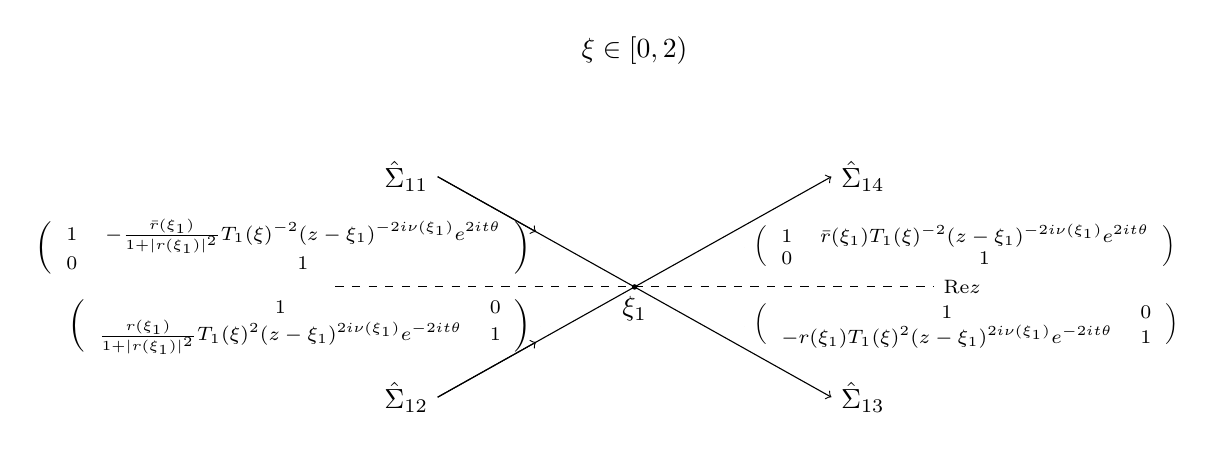
\begin{tikzpicture}[node distance=2cm]
      \draw[](0,2.7)node[above]{$\xi\in[0,2)$};
      \draw[->](0,0)--(2.5,1.4)node[right]{$\hat{\Sigma}_{14}$};
      \draw(0,0)--(-2.5,1.4)node[left]{$\hat{\Sigma}_{11}$};
      \draw(0,0)--(-2.5,-1.4)node[left]{$\hat{\Sigma}_{12}$};
      \draw[->](0,0)--(2.5,-1.4)node[right]{$\hat{\Sigma}_{13}$};
      \draw[dashed](-3.8,0)--(3.8,0)node[right]{\scriptsize Re$z$};
      \draw[->](-2.5,-1.4)--(-1.25,-0.7);
      \draw[->](-2.5,1.4)--(-1.25,0.7);
      \coordinate (A) at (-1.2,0.5);
      \coordinate (B) at (-1.2,-0.5);
      \coordinate (G) at (1.4,0.5);
      \coordinate (H) at (1.4,-0.5);
      \coordinate (I) at (0,0);
      \fill (A) circle (0pt) node[left] {\scriptsize$\left(
      \begin{array}{cc}
         1 & -\frac{\bar{r}(\xi_1)}{1+|r(\xi_1)|^2}T_1(\xi)^{-2}(z-\xi_1)^{-2i\nu(\xi_1)}e^{2it\theta}\\
         0 & 1
      \end{array}
      \right)$};
      \fill (B) circle (0pt) node[left] {\scriptsize$\left(
      \begin{array}{cc}
         1 & 0\\
         \frac{r(\xi_1)}{1+|r(\xi_1)|^2}T_1(\xi)^{2}(z-\xi_1)^{2i\nu(\xi_1)}e^{-2it\theta} & 1
      \end{array}
      \right)$};
      \fill (G) circle (0pt) node[right] {\scriptsize$\left(
      \begin{array}{cc}
         1& \bar{r}(\xi_1)T_1(\xi)^{-2}(z-\xi_1)^{-2i\nu(\xi_1)}e^{2it\theta}\\
         0&1
      \end{array}
      \right)$};
      \fill (H) circle (0pt) node[right] {\scriptsize$\left(
      \begin{array}{cc}
         1 & 0\\
         -r(\xi_1)T_1(\xi)^{2}(z-\xi_1)^{2i\nu(\xi_1)}e^{-2it\theta} & 1
      \end{array}
      \right)$};
      \fill (I) circle (1pt) node[below] {$\xi_1$};
   \end{tikzpicture}
   }
   \subfigure[]{
   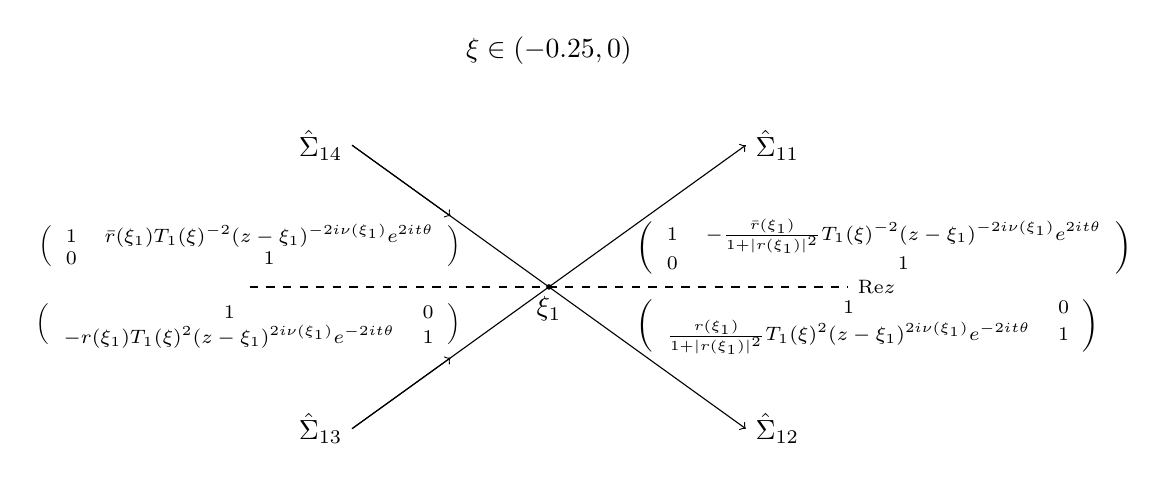
\begin{tikzpicture}[node distance=2cm]
      \draw[](0,2.7) node[above]{$\xi\in(-0.25,0)$};
      \draw[->](0,0)--(2.5,1.8)node[right]{$\hat{\Sigma}_{11}$};
      \draw(0,0)--(-2.5,1.8)node[left]{$\hat{\Sigma}_{14}$};
      \draw(0,0)--(-2.5,-1.8)node[left]{$\hat{\Sigma}_{13}$};
      \draw[->](0,0)--(2.5,-1.8)node[right]{$\hat{\Sigma}_{12}$};
      \draw[dashed](-3.8,0)--(3.8,0)node[right]{\scriptsize Re$z$};
      \draw[->](-2.5,-1.8)--(-1.25,-0.9);
      \draw[->](-2.5,1.8)--(-1.25,0.9);
      \coordinate (A) at (1,0.5);
      \coordinate (B) at (1,-0.5);
      \coordinate (G) at (-1,0.5);
      \coordinate (H) at (-1,-0.5);
      \coordinate (I) at (0,0);
      \fill (A) circle (0pt) node[right] {\scriptsize$\left(
      \begin{array}{cc}
         1 & -\frac{\bar{r}(\xi_1)}{1+|r(\xi_1)|^2}T_1(\xi)^{-2}(z-\xi_1)^{-2i\nu(\xi_1)}e^{2it\theta}\\
         0 & 1
      \end{array}
      \right)$};
      \fill (B) circle (0pt) node[right] {\scriptsize$\left(
      \begin{array}{cc}
         1 & 0\\
         \frac{r(\xi_1)}{1+|r(\xi_1)|^2}T_1(\xi)^{2}(z-\xi_1)^{2i\nu(\xi_1)}e^{-2it\theta} & 1
      \end{array}
      \right)$};
      \fill (G) circle (0pt) node[left] {\scriptsize$\left(
      \begin{array}{cc}
         1& \bar{r}(\xi_1)T_1(\xi)^{-2}(z-\xi_1)^{-2i\nu(\xi_1)}e^{2it\theta}\\
         0&1
      \end{array}
      \right)$};
      \fill (H) circle (0pt) node[left] {\scriptsize$\left(
      \begin{array}{cc}
         1 & 0\\
         -r(\xi_1)T_1(\xi)^{2}(z-\xi_1)^{2i\nu(\xi_1)}e^{-2it\theta} & 1
      \end{array}
      \right)$};
      \fill (I) circle (1pt) node[below] {$\xi_1$};
   \end{tikzpicture}
   }
   \caption{caption}\label{figS0}
\end{figure}



\clearpage



\begin{figure}
   \centering
   \subfigure[]{
   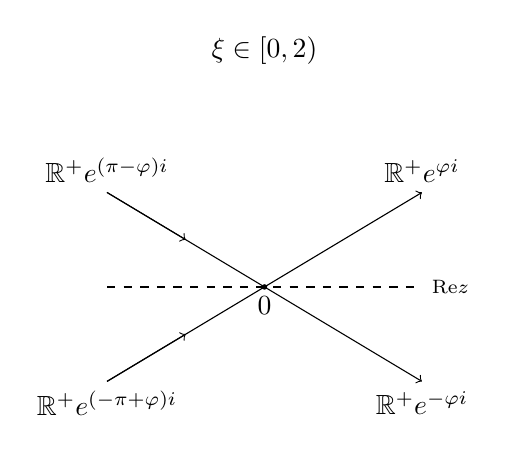
\begin{tikzpicture}[node distance=2cm]
      \draw[](0,2.7)node[above]{$\xi\in[0,2)$};
      \draw[->](0,0)--(2,1.2)node[above]{$\mathbb{R}^+e^{\varphi i}$};
      \draw(0,0)--(-2,1.2)node[above]{$\mathbb{R}^+e^{(\pi-\varphi)i}$};
      \draw(0,0)--(-2,-1.2)node[below]{$\mathbb{R}^+e^{(-\pi+\varphi)i}$};
      \draw[->](0,0)--(2,-1.2)node[below]{$\mathbb{R}^+e^{-\varphi i}$};
      \draw[dashed](-2,0)--(2,0)node[right]{\scriptsize Re$z$};
      \draw[->](-2,-1.2)--(-1,-0.6);
      \draw[->](-2,1.2)--(-1,0.6);
      \coordinate (A) at (-1.2,0.5);
      \coordinate (B) at (-1.2,-0.5);
      \coordinate (G) at (1.4,0.5);
      \coordinate (H) at (1.4,-0.5);
      \coordinate (I) at (0,0);
      \fill (I) circle (1pt) node[below] {$0$};
   \end{tikzpicture}
   }
   \subfigure[]{
   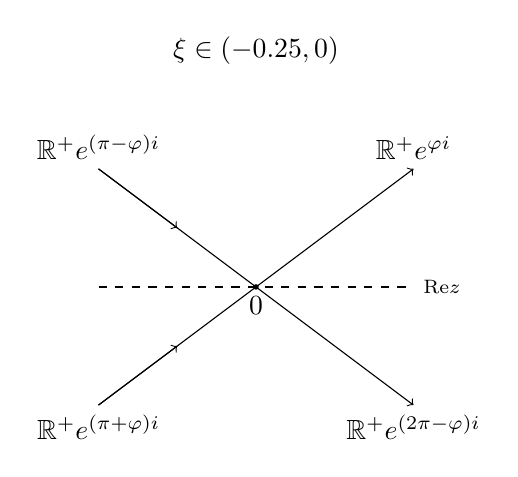
\begin{tikzpicture}[node distance=2cm]
      \draw[](0,2.7) node[above]{$\xi\in(-0.25,0)$};
      \draw[->](0,0)--(2,1.5)node[above]{$\mathbb{R}^+e^{\varphi i}$};
      \draw(0,0)--(-2,1.5)node[above]{$\mathbb{R}^+e^{(\pi-\varphi)i}$};
      \draw(0,0)--(-2,-1.5)node[below]{$\mathbb{R}^+e^{(\pi+\varphi)i}$};
      \draw[->](0,0)--(2,-1.5)node[below]{$\mathbb{R}^+e^{(2\pi-\varphi)i}$};
      \draw[dashed](-2,0)--(2,0)node[right]{\scriptsize Re$z$};
      \draw[->](-2,-1.5)--(-1,-0.75);
      \draw[->](-2,1.5)--(-1,0.75);
      \coordinate (A) at (1,0.5);
      \coordinate (B) at (1,-0.5);
      \coordinate (G) at (-1,0.5);
      \coordinate (H) at (-1,-0.5);
      \coordinate (I) at (0,0);
      \fill (I) circle (1pt) node[below] {$0$};
   \end{tikzpicture}
   }
   \caption{caption}\label{sigpc}
\end{figure}



\clearpage



\begin{figure}
   \centering
   \subfigure[]{
   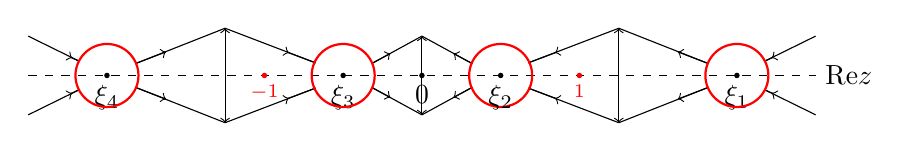
\begin{tikzpicture}
      \draw(4.35,0.18)--(5,0.5);
      \draw[-<](4.35,0.18)--(4.5,0.25);
      \draw(3.64,0.15)--(2.5,0.6);
      \draw[->](3.64,-0.15)--(3.25,-0.3);
      \draw(4.35,-0.18)--(5,-0.5);
      \draw[->](3.64,0.15)--(3.25,0.3);
      \draw(3.64,-0.15)--(2.5,-0.6);
      \draw[-<](4.35,-0.18)--(4.5,-0.25);
      \draw(-4.35,0.18)--(-5,0.5);
      \draw[-<](-4.35,0.18)--(-4.5,0.25);
      \draw(-3.64,0.15)--(-2.5,0.6);
      \draw[->](-3.64,-0.15)--(-3.25,-0.3);
      \draw(-4.35,-0.18)--(-5,-0.5);
      \draw[->](-3.64,0.15)--(-3.25,0.3);
      \draw(-3.64,-0.15)--(-2.5,-0.6);
      \draw[-<](-4.35,-0.18)--(-4.5,-0.25);
      \draw(-0.64,0.15)--(0,0.5);
      \draw[->](-0.64,0.15)--(-0.4,0.28);
      \draw(-1.35,0.16)--(-2.5,0.6);
      \draw[-<](-1.35,-0.16)--(-1.75,-0.31);
      \draw(-0.64,-0.15)--(0,-0.5);
      \draw[-<](-1.35,0.16)--(-1.75,0.31);
      \draw(-1.35,-0.16)--(-2.5,-0.6);
      \draw[->](-0.64,-0.15)--(-0.4,-0.28);
      \draw[dashed](-5,0)--(5,0)node[right]{ Re$z$};
      \draw(0.64,0.15)--(0,0.5);
      \draw[->](0.64,0.15)--(0.4,0.28);
      \draw(1.35,0.16)--(2.5,0.6);
      \draw[-<](1.35,-0.16)--(1.75,-0.31);
      \draw(0.64,-0.15)--(0,-0.5);
      \draw[-<](1.35,0.16)--(1.75,0.31);
      \draw(1.35,-0.16)--(2.5,-0.6);
      \draw[->](0.64,-0.15)--(0.4,-0.28);
      \draw[->](2.5,0)--(2.5,0.6);
      \draw[->](2.5,0)--(2.5,-0.6);
      \draw[->](-2.5,0)--(-2.5,0.6);
      \draw[->](-2.5,0)--(-2.5,-0.6);
      \draw[->](0,0)--(0,0.5);
      \draw[->](0,0)--(0,-0.5);
      \coordinate (I) at (0,0);
      \fill (I) circle (1pt) node[below] {$0$};
      \coordinate (A) at (-4,0);
      \fill (A) circle (1pt) node[below] {$\xi_4$};
      \coordinate (b) at (-1,0);
      \fill (b) circle (1pt) node[below] {$\xi_3$};
      \coordinate (e) at (4,0);
      \fill (e) circle (1pt) node[below] {$\xi_1$};
      \coordinate (f) at (1,0);
      \draw[thick,red](1,0) circle (0.4);
      \fill (f) circle (1pt) node[below] {$\xi_2$};
      \draw[thick,red](4,0) circle (0.4);
      \draw[thick,red](-1,0) circle (0.4);
      \draw[thick,red](-4,0) circle (0.4);
      \coordinate (c) at (-2,0);
      \fill[red] (c) circle (1pt) node[below] {\scriptsize$-1$};
      \coordinate (d) at (2,0);
      \fill[red] (d) circle (1pt) node[below] {\scriptsize$1$};
   \end{tikzpicture}
   }
   \subfigure[]{
   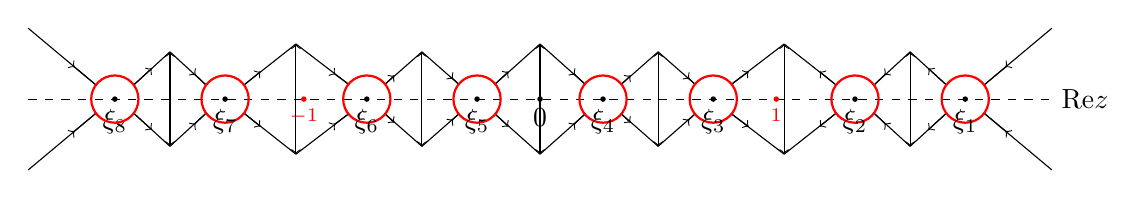
\begin{tikzpicture}
      \draw[dashed](-6.5,0)--(6.5,0)node[right]{ Re$z$};
      \coordinate (I) at (0,0);
      \fill (I) circle (1pt) node[below] {$0$};
      \coordinate (c) at (-3,0);
      \fill[red] (c) circle (1pt) node[below] {\scriptsize$-1$};
      \coordinate (D) at (3,0);
      \fill[red] (D) circle (1pt) node[below] {\scriptsize$1$};
      \draw(-0.575,0.187)--(-0,0.7);
      \draw[->](-0.575,0.187)--(-0.4,0.35);
      \draw(-1.03,0.186)--(-1.5,0.6);
      \draw[-<](-1.03,-0.186)--(-1.15,-0.3);
      \draw(-0.575,-0.187)--(-0,-0.7);
      \draw[-<](-1.03,0.186)--(-1.15,0.3);
      \draw(0.575,0.187)--(0,0.7);
      \draw[-<](0.575,0.187)--(0.4,0.35);
      \draw(1.03,0.186)--(1.5,0.6);
      \draw[->](1.03,-0.186)--(1.15,-0.3);
      \draw(0.575,-0.187)--(0,-0.7);
      \draw[->](1.03,0.186)--(1.15,0.3);
      \draw(1.03,-0.186)--(1.5,-0.6);
      \draw[-<](0.575,-0.187)--(0.4,-0.35);
      \draw(-1.03,-0.186)--(-1.5,-0.6);
      \draw[->](-0.575,-0.187)--(-0.4,-0.35);
      \draw(-1.97,0.187)--(-1.5,0.6);
      \draw[-<](-2.43,0.187)--(-2.65,0.35);
      \draw(-1.97,-0.187)--(-1.5,-0.6);
      \draw[->](-1.97,-0.187)--(-1.85,-0.3);
      \draw(-2.43,0.187)--(-3.1,0.7);
      \draw[->](-1.97,0.187)--(-1.85,0.3);
      \draw(-2.43,-0.187)--(-3.1,-0.7);
      \draw[-<](-2.43,-0.187)--(-2.65,-0.35);
      \draw(1.97,0.187)--(1.5,0.6);
      \draw[->](2.43,0.187)--(2.65,0.35);
      \draw(1.97,-0.187)--(1.5,-0.6);
      \draw[-<](1.97,-0.187)--(1.85,-0.3);
      \draw(2.43,0.187)--(3.1,0.7);
      \draw[-<](1.97,0.187)--(1.85,0.3);
      \draw(2.43,-0.187)--(3.1,-0.7);
      \draw[->](2.43,-0.187)--(2.65,-0.35);
      \draw(-5.64,0.18)--(-6.5,0.9);
      \draw[-<](-5.64,0.18)--(-5.96,0.446);
      \draw(-5.16,0.18)--(-4.7,0.6);
      \draw[->](-5.16,-0.18)--(-4.93,-0.39);
      \draw(-5.64,-0.18)--(-6.5,-0.9);
      \draw[->](-5.16,0.18)--(-4.93,0.39);
      \draw(-5.16,-0.18)--(-4.7,-0.6);
      \draw[-<](-5.64,-0.18)--(-5.96,-0.446);
      \draw(-3.75,0.187)--(-3.1,0.7);
      \draw[->](-3.75,0.187)--(-3.55,0.35);
      \draw(-4.25,0.187)--(-4.7,0.6);
      \draw[-<](-4.25,-0.187)--(-4.42,-0.35);
      \draw(-3.75,-0.187)--(-3.1,-0.7);
      \draw[-<](-4.25,0.187)--(-4.42,0.35);
      \draw(-4.25,-0.187)--(-4.7,-0.6);
      \draw[->](-3.75,-0.187)--(-3.55,-0.35);
      \draw(3.75,0.187)--(3.1,0.7);
      \draw[->](3.75,0.187)--(3.55,0.35);
      \draw(4.25,0.187)--(4.7,0.6);
      \draw[-<](4.25,-0.187)--(4.42,-0.35);
      \draw(3.75,-0.187)--(3.1,-0.7);
      \draw[-<](4.25,0.187)--(4.42,0.35);
      \draw(4.25,-0.187)--(4.7,-0.6);
      \draw[->](3.75,-0.187)--(3.55,-0.35);
      \draw[->](-1.5,0)--(-1.5,0.6);
      \draw[->](-1.5,0)--(-1.5,-0.6);
      \draw[->](-4.7,0)--(-4.7,0.6);
      \draw[->](-4.7,0)--(-4.7,-0.6);
      \draw[->](-3.1,0)--(-3.1,0.7);
      \draw[->](-3.1,0)--(-3.1,-0.7);
      \draw(5.64,0.18)--(6.5,0.9);
      \draw[-<](5.64,0.18)--(5.96,0.446);
      \draw(5.16,0.18)--(4.7,0.6);
      \draw[->](5.16,-0.18)--(4.93,-0.39);
      \draw(5.64,-0.18)--(6.5,-0.9);
      \draw[->](5.16,0.18)--(4.93,0.39);
      \draw(5.16,-0.18)--(4.7,-0.6);
      \draw[-<](5.64,-0.18)--(5.96,-0.446);
      \draw[->](1.5,0)--(1.5,0.6);
      \draw[->](1.5,0)--(1.5,-0.6);
      \draw[->](4.7,0)--(4.7,0.6);
      \draw[->](4.7,0)--(4.7,-0.6);
      \draw[->](3.1,0)--(3.1,0.7);
      \draw[->](3.1,0)--(3.1,-0.7);
      \draw[->](0,0)--(0,0.7);
      \draw[->](0,0)--(0,-0.7);
      \coordinate (A) at (-5.4,0);
      \fill (A) circle (1pt) node[below] {$\xi_8$};
      \draw[thick,red](-5.4,0) circle (0.3);
      \coordinate (b) at (-4,0);
      \draw[thick,red](-4,0) circle (0.3);
      \fill (b) circle (1pt) node[below] {$\xi_7$};
      \coordinate (C) at (-0.8,0);
      \draw[thick,red](-0.8,0) circle (0.3);
      \fill (C) circle (1pt) node[below] {$\xi_5$};
      \coordinate (d) at (-2.2,0);
      \draw[thick,red](-2.2,0) circle (0.3);
      \fill (d) circle (1pt) node[below] {$\xi_6$};
      \coordinate (E) at (5.4,0);
      \draw[thick,red](5.4,0) circle (0.3);
      \fill (E) circle (1pt) node[below] {$\xi_1$};
      \coordinate (R) at (4,0);
      \draw[thick,red](4,0) circle (0.3);
      \fill (R) circle (1pt) node[below] {$\xi_2$};
      \coordinate (T) at (0.8,0);
      \draw[thick,red](0.8,0) circle (0.3);
      \fill (T) circle (1pt) node[below] {$\xi_4$};
      \coordinate (Y) at (2.2,0);
      \draw[thick,red](2.2,0) circle (0.3);
      \fill (Y) circle (1pt) node[below] {$\xi_3$};
   \end{tikzpicture}
   }
   \caption{caption}\label{figE}
\end{figure}



\clearpage



\begin{figure}
   \begin{center}
      \begin{tikzpicture}[node distance=2cm]
         \draw[->](-4,0)--(4,0)node[right]{Re$z$};
         \draw[->](0,-3)--(0,3)node[above]{Im$z$};
         \draw[dashed] (2,0) arc (0:360:2);
         \coordinate (A) at (0,0);
         \coordinate (B) at (2,0);
         \coordinate (C) at (-2,0);
         \coordinate (G) at (-2.2,2.2);
         \coordinate (H) at (0,-2);
         \coordinate (I) at (0,2);
         \coordinate (J) at (1.414213562373095,1.414213562373095);
         \coordinate (K) at (1.414213562373095,-1.414213562373095);
         \coordinate (L) at (-1.414213562373095,1.414213562373095);
         \coordinate (M) at (-1.414213562373095,-1.414213562373095);
         \fill[blue] (A) circle (1.5pt) node[below right]  {\textcolor{black}{ $0$}  };
         \fill[green] (H) circle (1.5pt) node[below right] {\textcolor{black}{$-i$}};
         \fill[green] (I) circle (1.5pt) node[above right] {\textcolor{black}{$i$}};
         \fill[red] (J) circle (1.5pt) node[right] {\textcolor{black}{$z_n$}};
         \fill[red] (K) circle (1.5pt) node[right] {\textcolor{black}{$z_n^*$}};
         \fill[red] (L) circle (1.5pt) node[left] {\textcolor{black}{$-z_n^*$}};
         \fill[red] (M) circle (1.5pt) node[left] {\textcolor{black}{$-z_n$}};
         \fill[blue] (B) circle (1.5pt) node[below right] {\textcolor{black}{$1$}};
         \fill[blue] (C) circle (1.5pt) node[below left] {\textcolor{black}{$-1$}};
         \label{zplane2}
      \end{tikzpicture}
      \caption{caption}\label{discrete spectrum}
   \end{center}
\end{figure}



\clearpage



\begin{figure}
   \begin{center}
      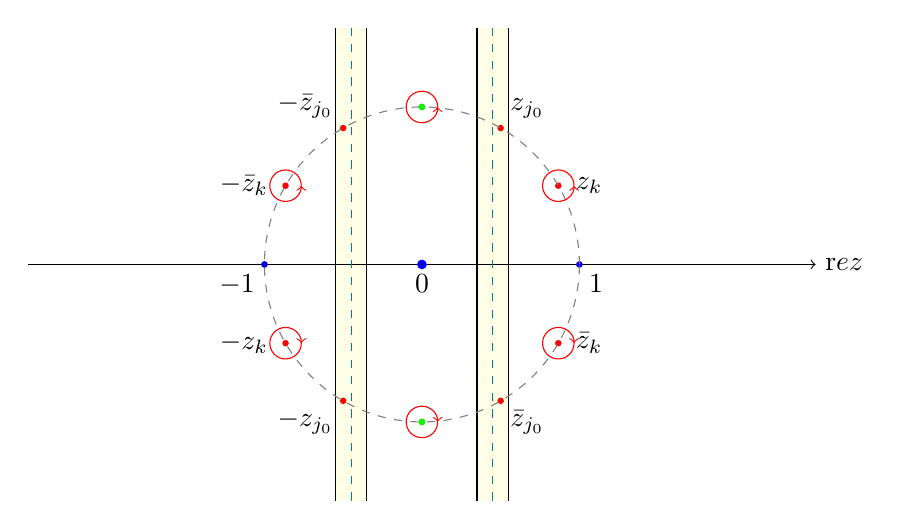
\begin{tikzpicture}[node distance=2cm]\label{Sigma1}
         \filldraw[yellow!10,line width=0.4] (0.7,-3) rectangle (1.1,3);
         \filldraw[yellow!10,line width=0.2] (-1.1,-3) rectangle (-0.7,3);
         \draw[->](-5,0)--(5,0)node[right]{${\mathrm re} z$};
         \draw (1.1,-3)--(1.1,3);
         \draw(0.7,-3)--(0.7,3);
         \draw (-1.1,-3)--(-1.1,3);
         \draw(-0.7,-3)--(-0.7,3);
         \draw[dashed,teal](0.9,-3)--(0.9,3);
         \draw[dashed,teal](-0.9,-3)--(-0.9,3);
         \node[below] at (0,0) {$0$};
         \node[shape=circle,fill=blue,scale=0.2] at (0,0) {$0$};
         \foreach \x [count=\p] in {0,...,11} {
         \node[shape=circle,fill=red, scale=0.25] (\p) at (-\x*30:2) {};};
                              % \foreach \x [count=\p] in {0,...,5} {
                                %   \draw (-\x*60:2.4) ;
                                 %  \draw (-30-\x*60:2.4) ;};
         \node[shape=circle,fill=blue, scale=0.25]  at (0:2) {};
         \node[shape=circle,fill=blue, scale=0.25]  at (-6*30:2) {};
         \node[right] at (1.83205,1) {$z_k$};
         \node[right] at (1.83205,-1) {$\bar{z}_k$};
         \node[left] at (-1.83205,1) {$-\bar{z}_k$};
         \node[left] at (-1.83205,-1) {$-z_k$};
         \node[above right] at (2*30:2) {$z_{j_0}$};
         \node[below right] at (-2*30:2) {$\bar{z}_{j_0}$};
         \node[above left] at (4*30:2) {$-\bar{z}_{j_0}$};
         \node[below left] at (-4*30:2) {$-z_{j_0}$};
         \draw [dashed, gray](1) arc (0:360:2);
         \draw[->,red] (1.93205,-1) arc(360:0:0.2);
         \draw[->,red] (1.93205,1) arc(0:360:0.2);
         \draw[->,red] (0.2,2) arc(0:360:0.2);
         \draw[->,red] (0.2,-2) arc(360:0:0.2);
         \draw[->,red] (-1.53205,1) arc(0:360:0.2);
         \draw[->,red] (-1.53205,-1) arc(360:0:0.2);
         \node[below left] at (-2,0) {$-1$};
         \node[below right] at (2,0) {$1$};
         \coordinate (H) at (0,-2);
         \coordinate (I) at (0,2);
         \fill[green] (H) circle (1.2pt) node[below right] {};
         \fill[green] (I) circle (1.2pt) node[above right] {};
      \end{tikzpicture}
                  %\flushleft{\footnotesize {\bf Figure $\ref{Sigma1}$} The dotted lines are ${\mathrm re} z=\pm\xi_0$. We divide the discrete spectrum into three set: $\triangle\setminus\Lambda$, $\nabla\setminus\Lambda$ and $\Lambda$ and reserve the poles in $\Lambda$. }
      \caption{caption}\label{Sigma1}
   \end{center}
\end{figure}



\clearpage



\begin{figure}
   \begin{center}
      \begin{tikzpicture}[node distance=2cm]
         \filldraw[yellow!10,line width=2] (0,0)--(5,1)--(5,0)--(0,0);
         \node[black]at (3.5,0.3){$\Omega_1$} ;
         \filldraw[yellow!10,line width=2] (0,0)--(-5,1)--(-5,0)--(0,0);
         \node[black]at (-3.5,0.3){$\Omega_2$} ;
         \filldraw[blue!10,line width=2] (0,0)--(5,-1)--(5,0)--(0,0);
         \filldraw[blue!10,line width=2] (0,0)--(-5,-1)--(-5,0)--(0,0);
         \node[black]at (-3.5,-0.3){$\Omega_3$} ;
         \node[black]at (3.5,-0.3){$\Omega_4$} ;
         \draw[->,dashed](-5,0)--(5,0)node[right]{${\mathrm re} z$};
         \draw (1.1,-3)--(1.1,3);
         \draw(0.7,-3)--(0.7,3);
         \draw (-1.1,-3)--(-1.1,3);
         \draw(-0.7,-3)--(-0.7,3);
         \draw[dashed,teal](0.9,-3)--(0.9,3);
         \draw[dashed,teal](-0.9,-3)--(-0.9,3);
         \draw[](0,0)--(5,1)node[above,black]{$\Sigma_1$};
         \draw[](0,0)--(-5,-1)node[below,black]{$\Sigma_3$};
         \draw[](0,0)--(-5,1)node[above,black]{$\Sigma_2$};
         \draw[](0,0)--(5,-1)node[below,black]{$\Sigma_4$};
         \node[below] at (0,0) {$0$};
         \node[shape=circle,fill=blue,scale=0.15] at (0,0) {$0$};
         \foreach \x [count=\p] in {0,...,11} {
         \node[shape=circle,fill=red, scale=0.25]  at (-\x*30:2) {};};
         \node[shape=circle,fill=blue, scale=0.25]  at (0:2) {};
         \node[shape=circle,fill=blue, scale=0.25]  at (-6*30:2) {};
         \node[right] at (1.93205,1) {$z_k$};
         \node[right] at (1.93205,-1) {$\bar{z}_k$};
         \node[left] at (-1.93205,1) {$-\bar{z}_k$};
         \node[left] at (-1.93205,-1) {$-z_k$};
         \node[above][right] at (2*30:2) {$z_{j_0}$};
         \node[below][right] at (-2*30:2) {$\bar{z}_{j_0}$};
         \node[above][left] at (4*30:2) {$-\bar{z}_{j_0}$};
         \node[below][left] at (-4*30:2) {$-z_{j_0}$};
         \draw [dashed, gray](1) arc (0:360:2);
         \draw[->,red] (1.93205,-1) arc(360:0:0.2);
         \draw[->,red] (1.93205,1) arc(0:360:0.2);
         \draw[->,red] (0.2,2) arc(0:360:0.2);
         \draw[->,red] (0.2,-2) arc(360:0:0.2);
         \draw[->,red] (-1.53205,1) arc(0:360:0.2);
         \draw[->,red] (-1.53205,-1) arc(360:0:0.2);
         \coordinate (H) at (0,-2);
         \coordinate (I) at (0,2);
         \fill[green] (H) circle (1.2pt) node[below right] {};
         \fill[green] (I) circle (1.2pt) node[above right] {};
      \end{tikzpicture}
      \caption{caption}\label{Sigma3}
   \end{center}
\end{figure}



\clearpage



\begin{figure}
   \centering
   \begin{tikzpicture}
      \draw (-5,0)--(5,0);
      \node [below] at (3,0) {$z_0$};
      \node [below] at (-3,0) {$-z_0$};
      \filldraw (3,0) circle (1pt);
      \filldraw (-3,0) circle (1pt);
      \draw [red] (0,1)--(2,1/3);
      \draw (2,1/3)--(5,-2/3);
      \draw [red] (0,1)--(-2,1/3);
      \draw (-2,1/3)--(-5,-2/3);
      \draw [red] (0,-1)--(2,-1/3);
      \draw (2,-1/3)--(5,2/3);
      \draw [red] (0,-1)--(-2,-1/3);
      \draw (-2,-1/3)--(-5,2/3);
      \draw (3.4,0) arc (0:22:0.4);
      \node [right] at (3.3,0.1) {$\tiny\alpha$};
      \node [above] at (4.2,1/2) {$\bar{L}$};
      \node [below] at (4.2,-1/2) {$L$};
      \node [above,red] at (0,1) {$L_\epsilon$};
      \node [below,red] at (0,-1) {$\bar{L}_\epsilon$};
   \end{tikzpicture}
   \caption{caption}\label{deformedContour}
\end{figure}



\clearpage



\begin{figure}
   \centering
   \begin{tikzpicture}
      \draw (-5,0)--(5,0);
      \node [below] at (3,0) {$z_0$};
      \node [below] at (-3,0) {$-z_0$};
      \filldraw (3,0) circle (1pt);
      \filldraw (-3,0) circle (1pt);
      \draw [red,->] (0,1)--(2,1/3);
      \draw (2,1/3)--(5,-2/3);
      \draw [red] (0,1)--(-2,1/3);
      \draw [<-](-2,1/3)--(-5,-2/3);
      \draw [red,->] (0,-1)--(2,-1/3);
      \draw (2,-1/3)--(5,2/3);
      \draw [red] (0,-1)--(-2,-1/3);
      \draw [<-](-2,-1/3)--(-5,2/3);
      \draw [<-] (4,1/3)--(4.5,1/2);
      \draw [<-] (4,-1/3)--(4.5,-1/2);
      \draw [->] (-4,1/3)--(-4.5,1/2);
      \draw [->] (-4,-1/3)--(-4.5,-1/2);
      \draw (3.4,0) arc (0:22:0.4);
      \node [right] at (3.3,0.1) {$\tiny\alpha$};
      \node [above] at (4.2,1/2) {$\bar{L}$};
      \node [below] at (4.2,-1/2) {$L$};
      \node [above,red] at (0,1) {$L_\epsilon$};
      \node [below,red] at (0,-1) {$\bar{L}_\epsilon$};
      \node [above] at (5.1,0.1) {$\Omega_1$};
      \node [below] at (0,-0.3) {$\Omega_2$};
      \node [above] at (-5.1,0.1) {$\Omega_3$};
      \node [below] at (5.1,-0.1) {$\Omega_4$};
      \node [above] at (0,0.3) {$\Omega_5$};
      \node [below] at (-5.1,-0.1) {$\Omega_6$};
      \node [above] at (0.2,1.3) {$\Omega_7$};
      \node [below] at (0.2,-1.5) {$\Omega_8$};
                  %orienations
                  %\draw (0,1)->(2,1/3);
   \end{tikzpicture}
   \caption{caption}\label{deformRigen}
\end{figure}



\clearpage



\begin{figure}
   \centering
   \begin{tikzpicture}
      \draw (-5,0)--(5,0);
      \node [below] at (3,0) {$z_0$};
      \node [below] at (-3,0) {$-z_0$};
      \filldraw (3,0) circle (1pt);
      \filldraw (-3,0) circle (1pt);
      \draw [red,->] (0,1)--(2,1/3);
      \draw (2,1/3)--(5,-2/3);
      \draw [red] (0,1)--(-2,1/3);
      \draw [<-](-2,1/3)--(-5,-2/3);
      \draw [red,->] (0,-1)--(2,-1/3);
      \draw (2,-1/3)--(5,2/3);
      \draw [red] (0,-1)--(-2,-1/3);
      \draw [<-](-2,-1/3)--(-5,2/3);
      \draw [<-] (4,1/3)--(4.5,1/2);
      \draw [<-] (4,-1/3)--(4.5,-1/2);
      \draw [->] (-4,1/3)--(-4.5,1/2);
      \draw [->] (-4,-1/3)--(-4.5,-1/2);
      \draw (3.4,0) arc (0:22:0.4);
      \node [right]at (1,0.85)  {$w^e=R+h_2$};
      \node[right ] at (1,-0.95)  {$w^e=\overline{R+h_2}$};
      \node [right ]at (4.5,-0.4) {$w^e=R$};
      \node [right ]at (4.5,0.34) {$w^e=\bar{R}$};
      \node [right] at (3.3,0.1) {$\tiny\alpha$};
      \node [above] at (0,0) {$w^e=h_1(\bar{h}_1)$};
      \node [above] at (4.2,1/2) {$\bar{L}$};
      \node [below] at (4.2,-1/2) {$L$};
      \node [above,red] at (0,1) {$L_\epsilon$};
      \node [below,red] at (0,-1) {$\bar{L}_\epsilon$};
                  %     \node [above] at (5.1,0.1) {$\Omega_1$};
                  %     \node [below] at (0,-0.3) {$\Omega_2$};
                  %     \node [above] at (-5.1,0.1) {$\Omega_3$};
                  %     \node [below] at (5.1,-0.1) {$\Omega_4$};
                  %     \node [above] at (0,0.3) {$\Omega_5$};
                  %     \node [below] at (-5.1,-0.1) {$\Omega_6$};
                  %     \node [above] at (0.2,1.3) {$\Omega_7$};
                  %     \node [below] at (0.2,-1.5) {$\Omega_8$};
                  %orienations
                  %\draw (0,1)->(2,1/3);
   \end{tikzpicture}
   \caption{caption}\label{fig:truncate errors}
\end{figure}



\clearpage



\begin{figure}
   \centering
   \begin{tikzpicture}
                  %  \draw (-5,0)--(5,0);
      \node [below] at (3,0) {$z_0$};
      \node [below] at (-3,0) {$-z_0$};
      \filldraw (3,0) circle (1pt);
      \filldraw (-3,0) circle (1pt);
                  %\draw [red,->] (0,1)--(2,1/3);
      \draw (2,1/3)--(5,-2/3);
                  %\draw [red] (0,1)--(-2,1/3);
      \draw [<-](-2,1/3)--(-5,-2/3);
                  %  \draw [red,->] (0,-1)--(2,-1/3);
      \draw (2,-1/3)--(5,2/3);
                  %  \draw [red] (0,-1)--(-2,-1/3);
      \draw [<-](-2,-1/3)--(-5,2/3);
      \draw [<-] (4,1/3)--(4.5,1/2);
      \draw [<-] (4,-1/3)--(4.5,-1/2);
      \draw [->] (-4,1/3)--(-4.5,1/2);
      \draw [->] (-4,-1/3)--(-4.5,-1/2);
      \draw [->] (2,1/3)--(2.5,1/6);
      \draw [->] (2,-1/3)--(2.5,-1/6);
      \node [below] at (4,-1/2){$\Sigma'_B$};
      \node [below] at (-4,-1/2){$\Sigma'_A$};
      \node at (0,1) {$\Sigma'$};
   \end{tikzpicture}
   \caption{caption}\label{splitedCrosses}
\end{figure}



\clearpage



\begin{figure}
   \centering
   \begin{tikzpicture}[scale=0.6]
                  % coordinates
      \draw [<->](-2,-2)--(2,2);
      \draw (-3,-3)--(3,3);
      \draw [<->](-2,2)--(2,-2);
      \draw (-3,3)--(3,-3);
      \node [below] at (0,0) {0};
      \node  [right] at (3,3) {$\Sigma_A^2$};
      \node  [right] at (3,-3) {$\Sigma_A^1$};
      \node  [left] at (-3,3) {$\Sigma_A^3$};
      \node  [left] at (-3,-3) {$\Sigma_A^4$};
   \end{tikzpicture}
   \caption{caption}\label{fig:sigma_A}
\end{figure}



\clearpage



\begin{figure}
   \centering
   \begin{tikzpicture}[scale=0.6]
                  % coordinates
      \draw [<-<](-2,-2)--(2,2);
      \draw (-3,-3)--(3,3);
      \draw [<-<](-2,2)--(2,-2);
                  %  \draw [-<](0,0)--(2,2);
      \draw (-3,3)--(3,-3);
      \node [below] at (0,0) {0};
      \draw [<-<] (-2,0)--(2,0);
      \draw [-](-4,0)--(4,0);
      \node [right] at (2,1) {$\Omega_1^e$};
      \node [] at (0,2) {$\Omega_2^e$};
      \node [left] at (-2,1) {$\Omega_3^e$};
      \node [left] at (-2,-1) {$\Omega_4^e$};
      \node [] at (0,-2) {$\Omega_5^e$};
      \node [right] at (2,-1) {$\Omega_6^e$};
                  %  \node [right] at (2,1) {$\Omega_1$};
                  %  \node  [right] at (3,3) {$\Sigma_A^2$};
                  %  \node  [right] at (3,-3) {$\Sigma_A^1$};
                  %  \node  [left] at (-3,3) {$\Sigma_A^3$};
                  %  \node  [left] at (-3,-3) {$\Sigma_A^4$};
   \end{tikzpicture}
   \caption{caption}\label{fig:sigma_e}
\end{figure}



\clearpage



\begin{figure}
   \vspace*{-23mm}
   \begin{picture}
      (150,160)(-70,100)
      \setlength{\unitlength}{0.60mm}
      \linethickness{0,9pt}
      \put(30.00,123.00){\makebox(0,0)[cc]{$E_0$}}\put(30.00,76.00){\makebox(0,0)[cc]{$E^*_0$}}
      \put(30.00,120.00){\line(0,-1){40.00}}
      \put(45.00,114.00){\line(0,-1){28.00}}
      \put(60.00,125.00){\line(0,-1){50.00}}
      \put(80.00,114.00){\line(0,-1){28.00}}
      \put(110.00,110.00){\line(0,-1){20.00}}
      \put(150.00,118.00){\makebox(0,0)[cc]{$E_N$}}\put(150.00,81.00){\makebox(0,0)[cc]{$E^*_N$}}
      \put(150.00,115.00){\line(0,-1){30.00}}\put(150.00,110.0){\vector(0,-1){3.00}}\put(150.00, 90.0){\vector(0,-1){3.00}}
      \put(180.00,95.00){\makebox(0,0)[cc]{$\lambda=\mathrm{Re} z$}}
      \put(78.00,118.00){\makebox(0,0)[cc]{$E_j$}}
      \put(78.00,80.00){\makebox(0,0)[cc]{$E^*_j$}}
      \put(10.00,100.00){\vector(1,0){170.00}}
      \linethickness{1,2pt}
      \put(70.00,100.00){\vector(1,0){3.00}}\put(90.00,100.00){\vector(1,0){3.00}}
      \put(30.00,110.0){\vector(0,-1){3.00}}\put(30.00,90.0){\vector(0,-1){3.00}}
      \put(45.00,105.0){\vector(0,-1){3.00}}\put(45.00,95.0){\vector(0,-1){3.00}}
      \put(60.00,115.0){\vector(0,-1){3.00}}\put(60.00,85.0){\vector(0,-1){3.00}}
      \put(80.00,110.0){\vector(0,-1){3.00}}\put(80.00,95.0){\vector(0,-1){3.00}}
      \put(110.00,105.0){\vector(0,-1){3.00}}\put(110.00,95.0){\vector(0,-1){3.00}}
   \end{picture}
   \vskip-1cm \caption{caption}\label{fig1}
\end{figure}



\clearpage



\begin{figure}
   \begin{picture}
      (150,160)(-70,100)
      \setlength{\unitlength}{0.60mm}
      \linethickness{1,20pt}
      \put(10.00,100.00){\vector(1,0){170.00}}
      \linethickness{1,50pt}\put(70.00,100.00){\vector(1,0){7.00}}
      \put(30.00,120.00){\line(1,0){20.00}}
      \put(50.00,120.00){\line(1,1){20.00}}\put(60.00,130.00){\vector(1,1){7.00}}\put(60.00,70.00){\vector(-1,1){7.00}}
      \put(70.00,140.00){\line(1,0){20.00}}
      \put(90.00,140.00){\line(1,-1){10.00}}
      \put(100.00,130.00){\line(1,0){25.00}}
      \put(125.00,130.00){\line(1,-1){20.00}}
      \put(30.00,80.00){\line(1,0){20.00}}
      \put(50.00,80.00){\line(1,-1){20.00}}
      \put(70.00,60.00){\line(1,0){20.00}}
      \put(90.00,60.00){\line(1,1){10.00}}
      \put(100.00,70.00){\line(1,0){25.00}}
      \put(125.00,70.00){\line(1,1){20.00}}
      \put(145.00,90.00){\line(0,1){20.00}}
      \put(30.00,125.00){\makebox(0,0)[cc]{$E_0$}}\put(30.00,74.00){\makebox(0,0)[cc]{$\hat E_6=E^*_0$}}
      \put(150.00,115.00){\makebox(0,0)[cc]{$\tilde E$}}\put(150.00,85.00){\makebox(0,0)[cc]{$\tilde E^*$}}
      \put(115.00,135.00){\makebox(0,0)[cc]{$\Sigma_2$}}
      \put(90.00,132.00){\makebox(0,0)[cc]{$\Gamma_2$}}
      \put(95.00,145.00){\makebox(0,0)[cc]{$\hat E_1$}}
      \put(100.00,125.00){\makebox(0,0)[cc]{$E_2$}}
      \put(125.00,125.00){\makebox(0,0)[cc]{$\hat E_2$}}
      \put(180.00,95.00){\makebox(0,0)[cc]{$\lambda=\mathrm{Re} z$}}
   \end{picture}
   \caption{caption}\label{fig3}
\end{figure}



\clearpage



\begin{figure}
   \begin{center}
      \begin{tikzpicture}[scale=1.3,decoration={markings,mark=at position .67 with {\arrow[black,line width=0.8mm]{>}
         ;}}]
         \draw[->](-3.5,0)--(2,0) node[right]{$\Re z$};
         \draw[->](0,-3)--(0,3) node[above]{$\Im z$};
         
         \draw[postaction={decorate}, very thick] (1.9,-3)..controls (0.2,0)..(1.9,3) node[near end, right]{$\Gamma_0$};
         \draw[postaction={decorate}, very thick, rotate around={120:(0,0)}] (1.9,-3)..controls (0.2,0)..(1.9,3) node[near end, above]{$\Gamma_1$};
         \draw[postaction={decorate}, very thick, rotate around={-120:(0,0)}] (1.9,-3)..controls (0.2,0)..(1.9,3) node[near end, left]{$\Gamma_2$};
      \end{tikzpicture}
   \end{center}
   \caption{Contours $\Gamma_0$, $\Gamma_1$, $\Gamma_2$ for the case of a cubic potential ($d=2$)}
   \label{fig:contoursGamma}
\end{figure}



\clearpage



\begin{figure}
   \begin{center}
      \begin{tikzpicture}[scale=1.3,decoration={markings,mark=at position .67 with {\arrow[black,line width=0.8mm]{>}
         ;}}]
                  %\draw[->](-3,0)--(2.5,0) node[right]{$\Re z$};
                  %\draw[->](0,-3)--(0,3) node[above]{$\Im z$};
         
         \draw[postaction={decorate}, very thick] (0,0)--(1,0) node[right]{$x^*$};
         \draw[postaction={decorate}, very thick, rotate around={120:(0,0)}] (0,0)--(1,0) node[right]{$\omega x^*$};
         \draw[postaction={decorate}, very thick, rotate around={-120:(0,0)}] (0,0)--(1,0) node[right]{$\omega^2 x^*$};
         
         \draw[postaction={decorate}, very thick] (1,0)--(2.2,2) node[near end, right]{$\Gamma_1$};
         \draw[postaction={decorate}, very thick] (1,0)--(2.2,-2) node[near end, right]{$\Gamma_2$};
         
         \draw[postaction={decorate}, very thick, rotate around={120:(0,0)}] (1,0)--(2.2,2) node[near end, above]{$\Gamma_2$};
         \draw[postaction={decorate}, very thick, rotate around={120:(0,0)}] (1,0)--(2.2,-2) node[near end, left]{$\Gamma_0$};
         
         \draw[postaction={decorate}, very thick, rotate around={-120:(0,0)}] (1,0)--(2.2,2) node[near end, left]{$\Gamma_0$};
         \draw[postaction={decorate}, very thick, rotate around={-120:(0,0)}] (1,0)--(2.2,-2) node[near end, below]{$\Gamma_1$};
         
         \draw(0.2,0) node[above]{$\Sigma_1$};
         \draw(0,0) node[left]{$0$};
      \end{tikzpicture}
   \end{center}
   \caption{caption}
   \label{fig:deformedGamma}
\end{figure}



\clearpage



\begin{figure}
   \begin{center}
      \begin{tikzpicture}[scale=1.3,decoration={markings,mark=at position .67 with {\arrow[black,line width=0.8mm]{>}
         ;}}]
                  %\draw[->](-3,0)--(2.5,0) node[right]{$\Re z$};
                  %\draw[->](0,-3)--(0,3) node[above]{$\Im z$};
         
         \draw[postaction={decorate}, very thick] (0,0)--(1,0) node[below]{$x^*$};
         \draw[very thick] (0,0)--(1.5,0) node[right]{$\widehat{x}$};
         \draw[postaction={decorate}, very thick, rotate around={120:(0,0)}] (0,0)--(1,0) node[right]{$\omega x^*$};
         \draw[very thick, rotate around ={120:(0,0)}] (1,0)--(1.5,0) node[above]{$\omega \widehat{x}$};
         \draw[postaction={decorate}, very thick, rotate around={-120:(0,0)}] (0,0)--(1,0) node[right]{$\omega^2 x^*$};
         \draw[very thick, rotate around ={-120:(0,0)}] (1,0)--(1.5,0) node[below]{$\omega^2 \widehat{x}$};
         
         \draw[postaction={decorate},very thick,rotate around={-90:(1.5,0)}] (1.5,0) parabola (3.5,1.5);
         \draw[postaction={decorate},very thick,rotate around={90:(1.5,0)}] (1.5,0) parabola (3.5,-1.5);
         
         \draw[postaction={decorate},very thick,rotate around={30:(-0.75,1.3)}] (-0.75,1.3) parabola (1.25,2.8);
         \draw[postaction={decorate},very thick,rotate around={210:(-0.75,1.3)}] (-0.75,1.3) parabola (1.25,-0.2);
         \draw[postaction={decorate},very thick,rotate around={-210:(-0.75,-1.3)}] (-0.75,-1.3) parabola (1.25,0.2);
         \draw[postaction={decorate},very thick,rotate around={-30:(-0.75,-1.3)}] (-0.75,-1.3) parabola (1.25,-2.8);
         
         \draw(2.5,1.6) node[right]{$C_0^+$}; 
         \draw(2.5,-1.6) node[right]{$C_0^-$};
         
         \draw[rotate around={120:(0,0)}] (2.5,1.6) node[above]{$C_1^+$}; 
         \draw[rotate around={120:(0,0)}] (2.5,-1.6) node[left]{$C_1^-$};
         
         \draw[rotate around={-120:(0,0)}] (2.5,1.6) node[left]{$C_2^+$}; 
         \draw[rotate around={-120:(0,0)}] (2.5,-1.6) node[below]{$C_2^-$};
         
         \draw(0.2,0) node[above]{$\Sigma_1$};
         \draw(0,0) node[left]{$0$};
         
         \filldraw(1,0) circle (1pt);
         \filldraw[rotate around={120:(0,0)}](1,0) circle (1pt);
         \filldraw[rotate around={-120:(0,0)}](1,0) circle (1pt);
      \end{tikzpicture}
   \end{center}
   \caption{Deformed contours $\Gamma_0$, $\Gamma_1$, $\Gamma_2$.
   All contours are oriented away from~$0$.}
   \label{fig:deformedGamma}
\end{figure}



\clearpage



\begin{figure}
   \begin{center}
      \begin{tikzpicture}[scale=1.3,decoration={markings,mark=at position .67 with {\arrow[black,line width=0.8mm]{>}
         ;}}]
         
         \draw[postaction={decorate}, very thick] (0,0)--(1,0) node[below]{$x^*$};
         \draw[very thick] (0,0)--(1.5,0) node[right]{$\widehat{x}$};
         \draw[postaction={decorate}, very thick, rotate around={120:(0,0)}] (0,0)--(1,0) node[right]{$\omega x^*$};
         \draw[very thick, rotate around ={120:(0,0)}] (1,0)--(1.5,0); % node[above]{$\omega \widehat{x}$};
         \draw[postaction={decorate}, very thick, rotate around={-120:(0,0)}] (0,0)--(1,0) node[right]{$\omega^2 x^*$};
         \draw[very thick, rotate around ={-120:(0,0)}] (1,0)--(1.5,0); % node[below]{$\omega^2 \widehat{x}$};
         
         \draw[postaction={decorate}, very thick] (0,0)--(-3,0) node[near end, above]{$\Sigma_2$};
         \draw[postaction={decorate}, very thick, rotate around={120:(0,0)}] (0,0)--(-3,0) node[near end, left]{$\Sigma_2$};
         \draw[postaction={decorate}, very thick, rotate around={-120:(0,0)}] (0,0)--(-3,0) node[near end, left]{$\Sigma_2$};
         
         \draw(3,0) node{$S_0$}; \draw(2,2) node{$S_0$};  \draw(2,-2) node{$S_0$}; 
         \draw(-1.5,2.5) node{$S_1$}; \draw[rotate around={120:(0,0)}] (2,2) node{$S_1$}; 
         \draw[rotate around={120:(0,0)}] (2,-2) node{$S_1$};
         \draw(-1.5,-2.5) node{$S_2$}; \draw[rotate around={-120:(0,0)}] (2,2) node{$S_2$}; 
         \draw[rotate around={-120:(0,0)}] (2,-2) node{$S_2$};
         
         \draw[postaction={decorate},very thick,rotate around={-90:(1.5,0)}] (1.5,0) parabola (3.5,1.5);
         \draw[postaction={decorate},very thick,rotate around={90:(1.5,0)}] (1.5,0) parabola (3.5,-1.5);
         
         \draw[postaction={decorate},very thick,rotate around={30:(-0.75,1.3)}] (-0.75,1.3) parabola (1.25,2.8);
         \draw[postaction={decorate},very thick,rotate around={210:(-0.75,1.3)}] (-0.75,1.3) parabola (1.25,-0.2);
         \draw[postaction={decorate},very thick,rotate around={-210:(-0.75,-1.3)}] (-0.75,-1.3) parabola (1.25,0.2);
         \draw[postaction={decorate},very thick,rotate around={-30:(-0.75,-1.3)}] (-0.75,-1.3) parabola (1.25,-2.8);
         
         \draw(2.5,1.6) node[right]{$C_0^+$}; 
         \draw(2.5,-1.6) node[right]{$C_0^-$};
         
         \draw[rotate around={120:(0,0)}] (2.5,1.6) node[above]{$C_1^+$}; 
         \draw[rotate around={120:(0,0)}] (2.5,-1.6) node[left]{$C_1^-$};
         
         \draw[rotate around={-120:(0,0)}] (2.5,1.6) node[left]{$C_2^+$}; 
         \draw[rotate around={-120:(0,0)}] (2.5,-1.6) node[below]{$C_2^-$};
         
                  %\draw(0.5,0) node[above]{$\Sigma_1$};
                  %\draw(0,0) node[left]{$0$};
         
         \filldraw(1,0) circle (1pt);
         \filldraw[rotate around={120:(0,0)}](1,0) circle (1pt);
         \filldraw[rotate around={-120:(0,0)}](1,0) circle (1pt);
      \end{tikzpicture}
   \end{center}
   \caption{Contour $\Gamma_X$ for the RH problem for $X$ and the sectors $S_0$, $S_1$ and $S_2$.}
   \label{fig:contourGammaX}
\end{figure}



\clearpage



\begin{figure}
   \begin{center}
      \begin{tikzpicture}[scale=1.3,decoration={markings,mark=at position .67 with {\arrow[black,line width=0.8mm]{>}
         ;}}]
         
         \draw[very thick] (0,0)--(1,0) node[below]{$x^*$};
         \draw[very thick] (0,0)--(1.5,0); % node[right]{$\widehat{x}$};
         \draw[very thick, rotate around ={120:(0,0)}] (0,0)--(1.5,0); % node[above]{$\omega \widehat{x}$};
         \draw[very thick, rotate around ={-120:(0,0)}] (0,0)--(1.5,0); % node[below]{$\omega^2 \widehat{x}$};
         
         \draw[postaction={decorate}, very thick] (0,0)--(-3,0);
         \draw[postaction={decorate}, very thick, rotate around={120:(0,0)}] (0,0)--(-3,0);
         \draw[postaction={decorate}, very thick, rotate around={-120:(0,0)}] (0,0)--(-3,0);
         
         \draw[postaction={decorate},very thick,rotate around={-90:(1.5,0)}] (1.5,0) parabola (3.5,1.5);
         \draw[postaction={decorate},very thick,rotate around={90:(1.5,0)}] (1.5,0) parabola (3.5,-1.5);
         
         \draw[postaction={decorate},very thick,rotate around={30:(-0.75,1.3)}] (-0.75,1.3) parabola (1.25,2.8);
         \draw[postaction={decorate},very thick,rotate around={210:(-0.75,1.3)}] (-0.75,1.3) parabola (1.25,-0.2);
         \draw[postaction={decorate},very thick,rotate around={-210:(-0.75,-1.3)}] (-0.75,-1.3) parabola (1.25,0.2);
         \draw[postaction={decorate},very thick,rotate around={-30:(-0.75,-1.3)}] (-0.75,-1.3) parabola (1.25,-2.8);
         
         \draw(2.5,1.6) node[right]{$C_0^+$}; 
         \draw(2.5,-1.6) node[right]{$C_0^-$};
         \draw[rotate around={120:(0,0)}] (2.5,1.6) node[above]{$C_1^+$}; 
         \draw[rotate around={120:(0,0)}] (2.5,-1.6) node[left]{$C_1^-$};
         
         \draw[rotate around={-120:(0,0)}] (2.5,1.6) node[left]{$C_2^+$}; 
         \draw[rotate around={-120:(0,0)}] (2.5,-1.6) node[below]{$C_2^-$};
         
         \draw[postaction={decorate},very thick](0.25,0.4)--(0.4,0.4)--(0.6,0.35)--(0.8,0.2)--(1,0);
         \draw[postaction={decorate},very thick](0.25,-0.4)--(0.4,-0.4)--(0.6,-0.35)--(0.8,-0.2)--(1,0);
         \draw[postaction={decorate},very thick, rotate around={120:(0,0)}](0.25,0.4)--(0.4,0.4)--(0.6,0.35)--(0.8,0.2)--(1,0);
         \draw[postaction={decorate},very thick, rotate around={120:(0,0)}](0.25,-0.4)--(0.4,-0.4)--(0.6,-0.35)--(0.8,-0.2)--(1,0);
         \draw[postaction={decorate},very thick, rotate around={-120:(0,0)}](0.25,0.4)--(0.4,0.4)--(0.6,0.35)--(0.8,0.2)--(1,0);
         \draw[postaction={decorate},very thick, rotate around={-120:(0,0)}](0.25,-0.4)--(0.4,-0.4)--(0.6,-0.35)--(0.8,-0.2)--(1,0);
         
         \draw[postaction={decorate},  very thick] (0.2,0)--(2,2.4);
         \draw[postaction={decorate}, very thick] (0.2,0)--(2,-2.4);
         \draw[postaction={decorate},  very thick, rotate around={120:(0,0)}] (0.2,0)--(2,2.4);
         \draw[postaction={decorate},  very thick, rotate around={120:(0,0)}] (0.2,0)--(2,-2.4);
         \draw[postaction={decorate},  very thick, rotate around={-120:(0,0)}] (0.2,0)--(2,2.4);
         \draw[postaction={decorate},  very thick, rotate around={-120:(0,0)}] (0.2,0)--(2,-2.4);
         
         \draw(0.3,0.17) node[right]{\tiny $L_1^+$};
         \draw(0.3,-0.18) node[right]{\tiny $L_1^-$};
         \draw(-0.4,0.17) node[above]{\tiny $L_1^+$};
         \draw(-0.1,0.35) node[above]{\tiny $L_1^-$};
         \draw(-0.15,-0.35) node[below]{\tiny $L_1^+$};
         \draw(-0.4,-0.17) node[below]{\tiny $L_1^-$};
         
         \draw(1.4,2.5) node[left]{$L_2^+$};
         \draw(1.8,2.2) node[left]{$L_2^-$};
         \draw(-2.8,0.0) node[below]{$L_2^+$};
         \draw(-2.8,0.5) node[below]{$L_2^-$};
         \draw(1.8,-2.2) node[left]{$L_2^+$};
         \draw(1.4,-2.5) node[left]{$L_2^-$};
         \filldraw(1,0) circle (1pt);
         \filldraw[rotate around={120:(0,0)}](1,0) circle (1pt);
         \filldraw[rotate around={-120:(0,0)}](1,0) circle (1pt);
      \end{tikzpicture}
   \end{center}
   \caption{caption}
   \label{fig:lenses}
\end{figure}



\clearpage



\begin{figure}
   \begin{center}
      \begin{tikzpicture}[scale=1.3,decoration={markings,mark=at position .67 with {\arrow[black,line width=0.8mm]{>}
         ;}}]
         
                  %\draw[very thick] (0,0)--(1,0) node[below]{$x^*$};
         \draw[very thick] (1.2,0)--(1.5,0); % node[right]{$\widehat{x}$};
         \draw[very thick, rotate around ={120:(0,0)}] (1.2,0)--(1.5,0); % node[above]{$\omega \widehat{x}$};
         \draw[very thick, rotate around ={-120:(0,0)}] (1.2,0)--(1.5,0); % node[below]{$\omega^2 \widehat{x}$};
         
                  %\draw[postaction={decorate}, very thick] (0,0)--(-3,0);
                  %\draw[postaction={decorate}, very thick, rotate around={120:(0,0)}] (0,0)--(-3,0);
                  %\draw[postaction={decorate}, very thick, rotate around={-120:(0,0)}] (0,0)--(-3,0);
         
         \draw[postaction={decorate},very thick,rotate around={-90:(1.5,0)}] (1.5,0) parabola (3.5,1.5);
         \draw[postaction={decorate},very thick,rotate around={90:(1.5,0)}] (1.5,0) parabola (3.5,-1.5);
         
         \draw[postaction={decorate},very thick,rotate around={30:(-0.75,1.3)}] (-0.75,1.3) parabola (1.25,2.8);
         \draw[postaction={decorate},very thick,rotate around={210:(-0.75,1.3)}] (-0.75,1.3) parabola (1.25,-0.2);
         \draw[postaction={decorate},very thick,rotate around={-210:(-0.75,-1.3)}] (-0.75,-1.3) parabola (1.25,0.2);
         \draw[postaction={decorate},very thick,rotate around={-30:(-0.75,-1.3)}] (-0.75,-1.3) parabola (1.25,-2.8);
         
         \draw(2.5,1.6) node[right]{$C_0^+$}; 
         \draw(2.5,-1.6) node[right]{$C_0^-$};
         \draw[rotate around={120:(0,0)}] (2.5,1.6) node[above]{$C_1^+$}; 
         \draw[rotate around={120:(0,0)}] (2.5,-1.6) node[left]{$C_1^-$};
         
         \draw[rotate around={-120:(0,0)}] (2.5,1.6) node[left]{$C_2^+$}; 
         \draw[rotate around={-120:(0,0)}] (2.5,-1.6) node[below]{$C_2^-$};
         
         \draw[very thick](0.24,0.4)--(0.4,0.4)--(0.6,0.35)--(0.8,0.2)--(0.89,0.11); 
         \draw[very thick](0.24,-0.4)--(0.4,-0.4)--(0.6,-0.35)--(0.8,-0.2)--(0.89,-0.11); 
         \draw[very thick, rotate around={120:(0,0)}](0.24,0.4)--(0.4,0.4)--(0.6,0.35)--(0.8,0.2)--(0.89,0.11); 
         \draw[very thick, rotate around={120:(0,0)}](0.24,-0.4)--(0.4,-0.4)--(0.6,-0.35)--(0.8,-0.2)--(0.89,-0.11); 
         \draw[very thick, rotate around={-120:(0,0)}](0.24,0.4)--(0.4,0.4)--(0.6,0.35)--(0.8,0.2)--(0.89,0.11); 
         \draw[very thick, rotate around={-120:(0,0)}](0.24,-0.4)--(0.4,-0.4)--(0.6,-0.35)--(0.8,-0.2)--(0.89,-0.11); 
         
         \draw[postaction={decorate},  very thick] (0.2,0)--(2,2.4);
         \draw[postaction={decorate}, very thick] (0.2,0)--(2,-2.4);
         \draw[postaction={decorate},  very thick, rotate around={120:(0,0)}] (0.2,0)--(2,2.4);
         \draw[postaction={decorate},  very thick, rotate around={120:(0,0)}] (0.2,0)--(2,-2.4);
         \draw[postaction={decorate},  very thick, rotate around={-120:(0,0)}] (0.2,0)--(2,2.4);
         \draw[postaction={decorate},  very thick, rotate around={-120:(0,0)}] (0.2,0)--(2,-2.4);
         
                  %\filldraw(1,0) circle (1pt);
                  %\filldraw[rotate around={120:(0,0)}](1,0) circle (1pt);
                  %\filldraw[rotate around={-120:(0,0)}](1,0) circle (1pt);
         
         \draw[very thick](1,0) circle (5pt);
         \draw[very thick,rotate around={120:(0,0)}](1,0) circle (5pt);
         \draw[very thick,rotate around={-120:(0,0)}](1,0) circle (5pt);
      \end{tikzpicture}
   \end{center}
   \caption{Contour $\Gamma_R$ for the RH problem for $R$.}
   \label{fig:contourR}
\end{figure}



\clearpage



\begin{figure}
   \center
   \begin{tikzpicture}
      \coordinate [label=0: Im $k$] ()at (0,2.8);
      \coordinate [label=0: Re $k$] ()at (3,-0.2);
      \coordinate [label=0:] ()at (2,0.1);
      \coordinate [label=0:] ()at (-2.6,0.1);
      \path [fill=pink] (-3.5,2.5)--(3.5,2.5) to
      (3.5,0)--(-3.5,0);
      \coordinate [label=0: $\mathbb{C}^{+}$] ()at (1,1);
      \coordinate [label=0: $\mathbb{C}^{-}$] ()at (1,-1);
      \draw[->, ] (3,0)--(3.5,0);
      \draw[->,] (0,2)--(0,2.5);
      \draw[thin](0,2)--(0,-2.3);
      \draw[thin](3.5,0)--(-3.5,0);
   \end{tikzpicture}
   \caption{caption}\label{1t}
\end{figure}



\clearpage



\begin{figure}
   \centering
   \begin{tabular}{c c}
      \begin{tikzpicture}[scale=0.75]
         \path [fill=gray!30](-3,0) -- (-2,4) -- (3,4) -- (0,0)--(-3,0);
         \draw [thick](-3,0) -- (-2,4);
         \draw [thick](0,0) -- (3,4);
         \draw [help lines][->] (-4,0) -- (4,0);
         \draw [help lines][->] (-3.8,-0.2) -- (-3.8,4);
         \draw [fill] (-3,0) circle [radius=0.025];
         \draw [fill] (0,0) circle [radius=0.025];
         \node [below] at (-3,0) {$x_1$};
         \node [below] at (0,0) {$x_2$};
         \node [below] at (4,0) {$x$};
         \node [left] at (-4,4) {$t$};
         \node [above] at (-2,4) {$\scriptstyle{x-v_1 t = x_1}$};
         \node [above] at (3,4) {$\scriptstyle{x-v_2 t = x_2}$};
      \end{tikzpicture}
      & 
      \qquad
      \begin{tikzpicture}[scale=0.75]
         \path [fill=gray!30](-2,-0.2) -- (-2,4) -- (2,4) -- (2,-0.2)--(-2,-0.2);
         \draw[thick](-2,-0.2) -- (-2,4);
         \draw[thick](2,-0.2) -- (2,4);
         \draw[help lines][->] (-4,0.0) -- (4,0.0);
         %\draw[fill] (-2,0) circle [radius=0.025];
         %\draw[fill] (2,0) circle [radius=0.025];
         %% Soliton nodes
         \draw[fill] (3,.4) circle [radius=0.04];
         \draw[fill] (2.3,3) circle [radius=0.04];
         \draw[fill] (1.3,2) circle [radius=0.04];
         \draw[fill] (-.2,.5) circle [radius=0.04];
         \draw[fill] (-.8,1.8) circle [radius=0.04];
         \draw[fill] (-1.3,.3) circle [radius=0.04];
         \draw[fill] (-2.4,3.3) circle [radius=0.04];
         \draw[fill] (-3,.5) circle [radius=0.04];
         \draw[fill] (-3,2.4) circle [radius=0.04];
         %% soliton node labels
         \node [left] at (3,.4) {$\scriptstyle{z_1}$};
         \node [right] at (2.3,3) {$\scriptstyle{z_8}$};
         \node [left] at (1.3,2) {$\scriptstyle{z_5}$};
         \node [left] at (-.2,.5) {$\scriptstyle{z_2}$};
         \node [left] at (-.8,1.8) {$\scriptstyle{z_6}$};
         \node [left] at (-1.3,.3) {$\scriptstyle{z_3}$};
         \node [left] at (-2.4,3.3) {$\scriptstyle{z_9}$};
         \node [left] at (-3,.5) {$\scriptstyle{z_4}$};
         \node [left] at (-3,2.4) {$\scriptstyle{z_7}$};
         %% exterior figure labels
         \node [below] at (-2,0) {$\scriptstyle{-v_2/2 }$};
         \node [below] at (1.9,0) {$\scriptstyle{-v_1/2  }$};
         \node [right] at (4,.0) {$\Re z$};
         \node [right] at (-4,3.7) {$C$};
      \end{tikzpicture}
      \\
   \end{tabular}
   \caption{caption}
\end{figure}



\clearpage



\begin{figure}
   \centering
   \begin{tikzpicture}
      %\draw[help lines] (-6,-6) grid (6,6);
      \path [fill=gray!30] (0,0) -- (-4,4) -- (-6,4) -- (-6,-4) -- (-4,-4) -- (0,0);
      \path [fill=gray!30] (0,0) -- (4,4) -- (6,4) -- (6,-4) -- (4,-4) -- (0,0);
      \draw [help lines] (-6,0) -- (6,0);
      \draw [thick][->] (-4,4) -- (-2,2);
      \draw [thick] [->](-2,2)--(2,-2);
      \draw [thick] (2,-2) -- (4,-4);
      \draw [thick][->] (-4,-4) -- (-2,-2);
      \draw [thick][->] (-2,-2)--(2,2);
      \draw [thick] (2,2) -- (4,4);
      \draw[color=white, fill=white] (1.5,1.4) circle [radius=.2];
      \draw[color=white, fill=white] (1.5,-1.4) circle [radius=.2];
      \draw[color=white, fill=white] (-3.5,2.5) circle [radius=.2];
      \draw[color=white, fill=white] (-3.5,-2.5) circle [radius=.2];
      \draw[color=white, fill=white] (3,2) circle [radius=.2];
      \draw[color=white, fill=white] (3,-2) circle [radius=.2];
      \node at (3.5,3) {$\Sigma_{1}$};
      \node at (-3.5,3) {$\Sigma_{2}$};
      \node at (-3.5,-3) {$\Sigma_{3}$};
      \node at (3.5,-3) {$\Sigma_{4}$};
      \node [right] at (6,0) {$\Re{z}$};
      \draw [fill] (0,0) circle [radius=0.025];
      \node [below] at (0,0) {$\xi$};
      \node at (1,.4) {$\Omega_{1}$};
      \node at (0,1.08) {$\Omega_{2}$};
      \node at (-1,.4) {$\Omega_{3}$};
      \node at (-1,-.4) {$\Omega_{4}$};
      \node at (0,-1.08) {$\Omega_{5}$};
      \node at (1,-.4) {$\Omega_{6}$};
      \node at (4,1) {$W^{2} = \stril[0] {-\dbar R_1 e^{2it \theta}} $ };
      \node at (-4,1) {$W^{2} = \striu[0]{ -\dbar R_3 e^{-2it \theta}} $ };
      \node at (-4,-1) {$W^{2} = \stril[0]{ \dbar R_4 e^{2it \theta}} $ };
      \node at (4,-1) {$W^{2} = \striu[0]{ \dbar R_6 e^{-2it \theta }} $};
   \end{tikzpicture}
   \caption{caption}\label{fig:M2def}
\end{figure}



\clearpage



\begin{figure}
   \centering
   \begin{tikzpicture}
      \draw [help lines] (-2,0) -- (2,0);
      \draw [thick][->] (-2,2) -- (-1,1);
      \draw [thick] [->](-2,2)--(1,-1);
      \draw [thick] (-2,2) -- (2,-2);
      \draw [thick][->] (-2,-2) -- (-1,-1);
      \draw [thick][->] (-2,-2)--(1,1);
      \draw [thick] (-2,-2) -- (2,2);
      \node at (2.3,2) {$\Sigma_{1}$};
      \node at (-2.3,2) {$\Sigma_{2}$};
      \node at (-2.3,-2) {$\Sigma_{3}$};
      \node at (2.3,-2) {$\Sigma_{4}$};
      \node [right] at (2,0) {$\Re{\zeta}$};
      \draw [fill] (0,0) circle [radius=0.025];
      \node [below] at (0,-0.1) {$0$};
      \node at (1,.4) {$\Omega_{1}$};
      \node at (0,1.08) {$\Omega_{2}$};
      \node at (-1,.4) {$\Omega_{3}$};
      \node at (-1,-.4) {$\Omega_{4}$};
      \node at (0,-1.08) {$\Omega_{5}$};
      \node at (1,-.4) {$\Omega_{6}$};
   \end{tikzpicture}
   \caption{caption}
\end{figure}



\clearpage



\begin{figure}
   \centering
   \begin{tikzpicture}
      \draw (0,0)--(4,0);
      % \node [above] at (-1,2) {$\theta'=0$};
      % \draw [->](-1,2)--(0,0.1);
      \draw [fill] (0,0) circle [radius=0.05];
      \node [below] at (0,0) {$O$};
      % \node [below] at (2,0) {$I_{j+}$};
      % \node [below] at (-2,0) {$I_{j-}$};
      \draw [line width=0.3 mm] (0,0)--(4,1.5);
      \path [fill=gray,opacity=0.3] (0,0)--(3.8,0)--(3.8,3.8*3/8)--(0,0);
      % \draw (0.5,0) arc (0:27:0.4) ;
      % \node [right] at (0.5,0.1) { $\alpha$};
      \node [above] at (3.8,1.5) {$\Sigma_{1}$};
      \node [above] at (3,0.4) {$\Omega_+$};
      
      \draw [line width=0.3 mm] (0,0)--(4,-1.5);
      \path [fill=gray,opacity=0.6] (0,0)--(3.8,0)--(3.8,-3.8*3/8)--(0,0);
      \node [below] at (3.8,-1.5) {$\Sigma_{2}$};
      \node [below] at (3,-0.4) {$\Omega_-$};
      % \draw (-0.5,0) arc (180:180-27:0.4) ;
      \node [above] at (-1,1) {$\Omega$};
   \end{tikzpicture}
   \caption{Contour deformation}
   \label{idea of dbar steepest descent}
\end{figure}



\clearpage



\begin{figure}
   \centering
   \begin{tikzpicture}
      \draw (-4,0)--(4,0);
      \node [above] at (-1,2) {$\theta'=0$};
      \draw [->](-1,2)--(0,0.1);
      \draw [fill] (0,0) circle [radius=0.05];
      \node [below] at (0,0) {$z_j$};
      \node [below] at (2,0) {$I_{j+}$};
      \node [below] at (-2,0) {$I_{j-}$};
      \draw [line width=0.3 mm] (0,0)--(4,1.5);
      \path [fill=gray,opacity=0.3] (0,0)--(3.8,0)--(3.8,3.8*3/8)--(0,0);
      \draw (0.5,0) arc (0:27:0.4) ;
      \node [right] at (0.5,0.1) { $\alpha$};
      \node [above] at (3.8,1.5) {$\Sigma_{j,1}$};
      
      \draw [line width=0.3 mm] (0,0)--(-4,1.5);
      \path [fill=gray,opacity=0.6] (0,0)--(-3.8,0)--(-3.8,3.8*3/8)--(0,0);
      \draw (-0.5,0) arc (180:180-27:0.4) ;
      \node [above] at (-3.8,1.5) {$\Sigma_{j,2}$};
      
      \draw [line width=0.3 mm] (0,0)--(-4,-1.5);
      \path [fill=gray,opacity=0.3] (0,0)--(-3.8,0)--(-3.8,-3.8*3/8)--(0,0);
      \draw (-0.5,0) arc (180:180+27:0.4) ;
      \node [below] at (-3.8,-1.5) {$\Sigma_{j,3}$};
      
      \draw [line width=0.3 mm] (0,0)--(4,-1.5);
      \path [fill=gray,opacity=0.6] (0,0)--(3.8,0)--(3.8,-3.8*3/8)--(0,0);
      \node [below] at (3.8,-1.5) {$\Sigma_{j,4}$};
      %\draw (0.5,0) arc (0:-27:0.4) ;
      
      \node at (3,0.65) {$\Omega_{j,1}$} ;
      \node at (-3,0.65) {$\Omega_{j,3}$} ;
      \node at (-3,-0.65) {$\Omega_{j,4}$} ;
      \node at (3,-0.65) {$\Omega_{j,6}$} ;
      \node at (0,0.95) {$\Omega_{j,2}$} ;
      \node at (0,-0.95) {$\Omega_{j,5}$} ;
   \end{tikzpicture}
   \caption{Notations for studying signatures of $\Im(\theta(z))$ near $z_j$}
   \label{notation for Im theta}
\end{figure}



\clearpage



\begin{figure}
   \centering
   \begin{tikzpicture}
      \draw (-6,0)--(6,0);
      \draw [fill] (-4,0) circle [radius=0.05] node [below] {$z_j$};
      \draw [fill] (4,0) circle [radius=0.05] node [below] {$z_{j+1}$};
      \draw [fill] (0,0) circle [radius=0.05] node [below] {$z_{j+\frac{1}{2}}$};
      \draw (-4,0)--(0,2)--(4,0);
      \path [fill=gray,opacity=0.3] (-4,0)--(0,2)--(4,0)--(-4,0);
      \draw [red,line width=0.3 mm] (0,2)--(0,0);
      \draw [->] (2,2)--(0.1,1.5) ;
      \node [right] at (2,2) {$\Sigma_{j+\frac{1}{2}}$};
      \node at (-2,0.4) {$\Omega_{j,1}$};
      \node at (2,0.4) {$\Omega_{j+1,3}$};
      \node at (-4,1.2) {$\Omega_{j,2}$};
      \node at (4,1.2) {$\Omega_{j+1,2}$};
      \node [above] at (-2,1){$\Sigma_{j,1}$};
      \node [above] at (2,1){$\Sigma_{j+1,2}$};
   \end{tikzpicture}
   \caption{Jumps in a small triangular region.}
   \label{sigma j 1/2}
\end{figure}



\clearpage



\begin{figure}
   \centering
   \begin{tikzpicture}
      \draw [dashed,color=gray,opacity=0.3,line width=0.35 mm] (-6,0)--(6,0);
      \draw (-6,1/2)--(-2,-1.5);
      \draw (-6,-1/2)--(-2,1.5);
      \draw [dashed,color=gray,opacity=0.3,line width=0.35 mm](-2,-1.5)--(0,-2.5);
      \draw [dashed,color=gray,opacity=0.3,line width=0.35 mm](-2,1.5)--(0,2.5);
      \draw (6,-1/2)--(2,1.5);
      \draw (6,1/2)--(2,-1.5);
      \draw [dashed,color=gray,opacity=0.3,line width=0.35 mm](2,1.5)--(0,2.5);
      \draw [dashed,color=gray,opacity=0.3,line width=0.35 mm](2,-1.5)--(0,-2.5);
      \draw [dashed,color=gray,opacity=0.3,line width=0.35 mm](0,2.5)--(0,-2.5);
      \node [below] at (-5,-0.2) {$z_j$} ;
      \node [below] at (5,-0.2) {$z_{j+1}$};
      \node [above] at (-3.4,0.8) {$\Sigma_{j,1}^o$};
      \node [above] at (3.4,0.8) {$\Sigma_{j+1,2}^o$};
      \node [below] at (-3.4,-0.8) {$\Sigma_{j,4}^o$};
      \node [below] at (3.4,-0.9) {$\Sigma_{j+1,3}^o$};
   \end{tikzpicture}
   \caption{New contours, dashed line segments are those deleted parts.}
   \label{truncated contours}
\end{figure}



\clearpage



\begin{figure}
   \centering
   \begin{tikzpicture}
      \path [draw=blue,line width=0.3 mm,postaction={on each segment={mid arrow=red}}]
      (-3,0)--(-0.05,0)--(-0.05,1.5)--(-3,0);
      \path [draw=green,line width=0.3 mm,postaction={on each segment={mid arrow=red}}]
      (0.05,0)--(3,0)--(0.05,1.5)--(0.05,0);
      \draw [line width=0.2 mm](-4,0)--(4,0);
   \end{tikzpicture}
\end{figure}



\clearpage



\begin{figure}
   \centering
   \tikzset{every picture/.style={line width=0.75pt}} %set default line width to 0.75pt        
   \begin{tikzpicture}[x=0.75pt,y=0.75pt,yscale=-1,xscale=1]
      %uncomment if require: \path (0,480); %set diagram left start at 0, and has height of 480
      
      %Straight Lines [id:da033751413755709114] 
      \draw    (351,68.5) -- (351,95.5) ;
      \draw [shift={(351,97.5)}, rotate = 270] [color={rgb, 255:red, 0; green, 0; blue, 0 }  ][line width=0.75]    (10.93,-3.29) .. controls (6.95,-1.4) and (3.31,-0.3) .. (0,0) .. controls (3.31,0.3) and (6.95,1.4) .. (10.93,3.29)   ;
      %Straight Lines [id:da18304813914789442] 
      \draw    (352,125.5) -- (352,159.5) ;
      \draw [shift={(352,161.5)}, rotate = 270] [color={rgb, 255:red, 0; green, 0; blue, 0 }  ][line width=0.75]    (10.93,-3.29) .. controls (6.95,-1.4) and (3.31,-0.3) .. (0,0) .. controls (3.31,0.3) and (6.95,1.4) .. (10.93,3.29)   ;
      %Straight Lines [id:da08124002810273079] 
      \draw    (351,187.5) -- (351,219.5) ;
      \draw [shift={(351,221.5)}, rotate = 270] [color={rgb, 255:red, 0; green, 0; blue, 0 }  ][line width=0.75]    (10.93,-3.29) .. controls (6.95,-1.4) and (3.31,-0.3) .. (0,0) .. controls (3.31,0.3) and (6.95,1.4) .. (10.93,3.29)   ;
      %Straight Lines [id:da5217021068995016] 
      \draw    (259,221.5) -- (485,222.5) ;
      %Straight Lines [id:da8364406338125938] 
      \draw    (259,221.5) -- (259.95,259.5) ;
      \draw [shift={(260,261.5)}, rotate = 268.57] [color={rgb, 255:red, 0; green, 0; blue, 0 }  ][line width=0.75]    (10.93,-3.29) .. controls (6.95,-1.4) and (3.31,-0.3) .. (0,0) .. controls (3.31,0.3) and (6.95,1.4) .. (10.93,3.29)   ;
      %Straight Lines [id:da7120737338973813] 
      \draw    (485,222.5) -- (485,259.5) ;
      \draw [shift={(485,261.5)}, rotate = 270] [color={rgb, 255:red, 0; green, 0; blue, 0 }  ][line width=0.75]    (10.93,-3.29) .. controls (6.95,-1.4) and (3.31,-0.3) .. (0,0) .. controls (3.31,0.3) and (6.95,1.4) .. (10.93,3.29)   ;
      %Straight Lines [id:da9031479502675461] 
      \draw    (485,292.5) -- (485.94,323.5) ;
      \draw [shift={(486,325.5)}, rotate = 268.26] [color={rgb, 255:red, 0; green, 0; blue, 0 }  ][line width=0.75]    (10.93,-3.29) .. controls (6.95,-1.4) and (3.31,-0.3) .. (0,0) .. controls (3.31,0.3) and (6.95,1.4) .. (10.93,3.29)   ;
      %Straight Lines [id:da8841466640758846] 
      \draw    (487,354.5) -- (487.93,380.5) ;
      \draw [shift={(488,382.5)}, rotate = 267.95] [color={rgb, 255:red, 0; green, 0; blue, 0 }  ][line width=0.75]    (10.93,-3.29) .. controls (6.95,-1.4) and (3.31,-0.3) .. (0,0) .. controls (3.31,0.3) and (6.95,1.4) .. (10.93,3.29)   ;
      %Straight Lines [id:da1714904266864925] 
      \draw    (488,404.5) -- (489.86,430.51) ;
      \draw [shift={(490,432.5)}, rotate = 265.90999999999997] [color={rgb, 255:red, 0; green, 0; blue, 0 }  ][line width=0.75]    (10.93,-3.29) .. controls (6.95,-1.4) and (3.31,-0.3) .. (0,0) .. controls (3.31,0.3) and (6.95,1.4) .. (10.93,3.29)   ;
      %Curve Lines [id:da33641820418844515] 
      \draw    (472,449.5) .. controls (434.38,430.69) and (418.32,313.87) .. (456.82,282.43) ;
      \draw [shift={(458,281.5)}, rotate = 503.13] [color={rgb, 255:red, 0; green, 0; blue, 0 }  ][line width=0.75]    (10.93,-3.29) .. controls (6.95,-1.4) and (3.31,-0.3) .. (0,0) .. controls (3.31,0.3) and (6.95,1.4) .. (10.93,3.29)   ;
      %Curve Lines [id:da14429246801857087] 
      \draw    (263,289.5) .. controls (302,323.5) and (420,305.5) .. (460,275.5) ;
      %Straight Lines [id:da5788083203930596] 
      \draw    (360,306.5) -- (277.91,331.91) ;
      \draw [shift={(276,332.5)}, rotate = 342.8] [color={rgb, 255:red, 0; green, 0; blue, 0 }  ][line width=0.75]    (10.93,-3.29) .. controls (6.95,-1.4) and (3.31,-0.3) .. (0,0) .. controls (3.31,0.3) and (6.95,1.4) .. (10.93,3.29)   ;
      %Curve Lines [id:da9826744196105175] 
      \draw    (595,234.5) .. controls (557.57,251.25) and (525.96,253.44) .. (525.02,289.81) ;
      \draw [shift={(525,291.5)}, rotate = 270] [color={rgb, 255:red, 0; green, 0; blue, 0 }  ][line width=0.75]    (10.93,-3.29) .. controls (6.95,-1.4) and (3.31,-0.3) .. (0,0) .. controls (3.31,0.3) and (6.95,1.4) .. (10.93,3.29)   ;
      %Curve Lines [id:da14112929848257583] 
      \draw    (595,234.5) .. controls (652.13,331.03) and (569.55,326.66) .. (541.25,353.26) ;
      \draw [shift={(540,354.5)}, rotate = 313.96000000000004] [color={rgb, 255:red, 0; green, 0; blue, 0 }  ][line width=0.75]    (10.93,-3.29) .. controls (6.95,-1.4) and (3.31,-0.3) .. (0,0) .. controls (3.31,0.3) and (6.95,1.4) .. (10.93,3.29)   ;
      %Curve Lines [id:da9949936335253704] 
      \draw    (595,234.5) .. controls (688.53,270.32) and (635.54,350.69) .. (586.74,402.72) ;
      \draw [shift={(586,403.5)}, rotate = 313.3] [color={rgb, 255:red, 0; green, 0; blue, 0 }  ][line width=0.75]    (10.93,-3.29) .. controls (6.95,-1.4) and (3.31,-0.3) .. (0,0) .. controls (3.31,0.3) and (6.95,1.4) .. (10.93,3.29)   ;
      
      % Text Node
      \draw (350.5,50.25) node   [align=left] {
      \begin{minipage}[lt]
         {55.08pt}\setlength\topsep{0pt}
         $ $$\displaystyle m^{[ 0]} =m$
      \end{minipage}
      };
      % Text Node
      \draw (366,110) node   [align=left] {
      \begin{minipage}[lt]
         {88pt}\setlength\topsep{0pt}
         $\displaystyle m^{[1]} =m^{[ 0]} \delta ^{\sigma _{3}}$
      \end{minipage}
      };
      % Text Node
      \draw (353,71.5) node [anchor=north west][inner sep=0.75pt]   [align=left] {Conjugation};
      % Text Node
      \draw (367,180) node   [align=left] {
      \begin{minipage}[lt]
         {88pt}\setlength\topsep{0pt}
         $\displaystyle m^{[ 2]} =m^{[ 1]} O( z)$
      \end{minipage}
      };
      % Text Node
      \draw (354,128.5) node [anchor=north west][inner sep=0.75pt]   [align=left] {Open lenses};
      % Text Node
      \draw (353,190.5) node [anchor=north west][inner sep=0.75pt]   [align=left] {Mixed $\displaystyle \overline{\partial }$-RHP};
      % Text Node
      \draw (224,263) node [anchor=north west][inner sep=0.75pt]   [align=left] {$\displaystyle \overline{\partial }$-Problem};
      % Text Node
      \draw (489,279.75) node   [align=left] {
      \begin{minipage}[lt]
         {35.36pt}\setlength\topsep{0pt}
         $\displaystyle m_{RHP}^{[ 2]}$
      \end{minipage}
      };
      % Text Node
      \draw (545.5,308.75) node   [align=left] {
      \begin{minipage}[lt]
         {82.28pt}\setlength\topsep{0pt}
         Remove $\displaystyle \Sigma _{j+1/2}$
      \end{minipage}
      };
      % Text Node
      \draw (492.5,339.75) node   [align=left] {
      \begin{minipage}[lt]
         {27.88pt}\setlength\topsep{0pt}
         $\displaystyle \tilde{m}^{[ 2]}$
      \end{minipage}
      };
      % Text Node
      \draw (499,393.13) node   [align=left] {
      \begin{minipage}[lt]
         {34pt}\setlength\topsep{0pt}
         $\displaystyle \hat{m}^{[ 2]}$
      \end{minipage}
      };
      % Text Node
      \draw (531,368.25) node   [align=left] {
      \begin{minipage}[lt]
         {58.48pt}\setlength\topsep{0pt}
         Localization
      \end{minipage}
      };
      % Text Node
      \draw (500.5,446.25) node   [align=left] {
      \begin{minipage}[lt]
         {31.96pt}\setlength\topsep{0pt}
         $\displaystyle m^{[ 3]}$
      \end{minipage}
      };
      % Text Node
      \draw (496,407) node [anchor=north west][inner sep=0.75pt]   [align=left] {{\scriptsize Reduce phase \& separate contributions}};
      % Text Node
      \draw (426.5,435.75) node [font=\small]   [align=left] {
      \begin{minipage}[lt]
         {49.64pt}\setlength\topsep{0pt}
         Existence
      \end{minipage}
      };
      % Text Node
      \draw (400.5,338.25) node  [font=\small] [align=left] {
      \begin{minipage}[lt]
         {60.52pt}\setlength\topsep{0pt}
         Small norm\\
         (for large $\displaystyle t$)
      \end{minipage}
      };
      % Text Node
      \draw (264,363) node   [align=left] {
      \begin{minipage}[lt]
         {128pt}\setlength\topsep{0pt}
         $\displaystyle E=m^{[ 2]}\left( m_{RHP}^{[ 2]}\right)^{-1}$
      \end{minipage}
      };
      % Text Node
      \draw (279,304) node [anchor=north west][inner sep=0.75pt]   [align=left] {\textcolor[rgb]{0.94,0.05,0.05}{Error}};
      % Text Node
      \draw (583,214) node [anchor=north west][inner sep=0.75pt]   [align=left] {\textcolor[rgb]{0.94,0.05,0.05}{Error}};
      % Text Node
      \draw (570.5,223.25) node  [font=\footnotesize] [align=left] {
      \begin{minipage}[lt]
         {42.84pt}\setlength\topsep{0pt}
         $\displaystyle \mathcal{O}\left( t^{-1}\right)$
      \end{minipage}
      };
      % Text Node
      \draw (254,312.75) node  [font=\footnotesize] [align=left] {
      \begin{minipage}[lt]
         {46.24pt}\setlength\topsep{0pt}
         $\displaystyle \mathcal{O}\left( t^{-3/4}\right)$
      \end{minipage}
      };
   \end{tikzpicture}
   \caption{Steps of the $\dbar$-steepest method.}
   \label{fig:steps}
\end{figure}


\clearpage


\begin{figure}
   \centering
   \begin{tikzpicture}
      \path [draw=black,postaction={on each segment={mid arrow=red}}] (-5,0)--(-2,0)--(2,0)--(5,0);
      \node[circle, fill=red, scale=0.3]  at (2,0) {};
      \node[circle, fill=red, scale=0.3]  at (-2,0) {};
      \node[below left] at (2,0) {\small $\xi_0$};
      \node[below right] at (-2,0) {\small $-\xi_0$};
      \path [draw=blue,postaction={on each segment={mid arrow=red}}] (2,0) -- (4.8,2); 
      \path [draw=blue,postaction={on each segment={mid arrow=red}}] (2,0) -- (4.8,-2); 
      \path [draw=blue,postaction={on each segment={mid arrow=red}}] (-4.8,2)--(-2,0) ; 
      \path [draw=blue,postaction={on each segment={mid arrow=red}}] (-4.8,-2)--(-2,0); 
      \node [right] at (4.2,1.5) {$\Sigma_1$};
      \node [left] at (-4.2,1.5) {$\Sigma_2$};
      \node [left] at (-4.2,-1.5) {$\Sigma_3$};
      \node [right] at (4.2,-1.5) {$\Sigma_4$};
      \node [below] at (0,0) {$\Sigma_0$};
      \node [right] at (3.2,0.5) {$\Omega_1$};
      \node [above] at (0,0.5) {$\Omega_2$};
      \node [left] at (-3.2,0.5) {$\Omega_3$};
      \node [left] at (-3.2,-0.5) {$\Omega_4$};
      \node [below] at (0,-1.2) {$\Omega_5$};
      \node [right] at (3.2,-0.5) {$\Omega_6$};
   \end{tikzpicture}
   \caption{Contour for $\dbar$-RHP.}
   \label{painleve region contours}
\end{figure}



\clearpage



\begin{figure}
   \centering
   \begin{tikzpicture}
      \path [draw=black,postaction={on each segment={mid arrow=red}}] (-2,0)--(2,0);
      \node[circle, fill=red, scale=0.3]  at (2,0) {};
      \node[circle, fill=red, scale=0.3]  at (-2,0) {};
      \node[below left] at (2.2,0) {\small $|\xi_0|$};
      \node[below right] at (-2.2,0) {\small $-|\xi_0|$};
      \path [draw=blue,postaction={on each segment={mid arrow=red}}] (2,0) -- (4.8,2); 
      \path [draw=green,postaction={on each segment={mid arrow=red}}] (0,0) -- (2.8,2); 
      \path [draw=blue,postaction={on each segment={mid arrow=red}}] (2,0) -- (4.8,-2); 
      \path [draw=green,postaction={on each segment={mid arrow=red}}] (0,0) -- (2.8,-2); 
      \path [draw=blue,postaction={on each segment={mid arrow=red}}] (-4.8,2)--(-2,0) ; 
      \path [draw=blue,postaction={on each segment={mid arrow=red}}] (-4.8,-2)--(-2,0); 
      \path [draw=green,postaction={on each segment={mid arrow=red}}] (-2.8,2)--(0,0) ; 
      \path [draw=green,postaction={on each segment={mid arrow=red}}] (-2.8,-2)--(0,0); 
      \node [right] at (4.2,1.5) {$\Sigma_1$};
      \node [right] at (2.2,1.5) {$\Sigma_1^{[5]}$};
      \node [left] at (-4.2,1.5) {$\Sigma_2$};
      \node [left] at (-2.2,1.5) {$\Sigma_2^{[5]}$};
      \node [left] at (-4.2,-1.5) {$\Sigma_3$};
      \node [left] at (-2.2,-1.5) {$\Sigma_3^{[5]}$};
      \node [right] at (4.2,-1.5) {$\Sigma_4$};
      \node [right] at (2.2,-1.5) {$\Sigma_4^{[5]}$};
       % \node [below] at (0,0) {$\Sigma_0$};
       % \node [right] at (3.2,0.5) {$\Omega_1$};
       % \node [above] at (0,0.5) {$\Omega_2$};
       % \node [left] at (-3.2,0.5) {$\Omega_3$};
       % \node [left] at (-3.2,-0.5) {$\Omega_4$};
       % \node [below] at (0,-1.2) {$\Omega_5$};
       % \node [right] at (3.2,-0.5) {$\Omega_6$};
   \end{tikzpicture}
   \caption{Contour for $m^{[4]}$(Green part).}
   \label{Countors for Painleve II hierarchy}
\end{figure}

\end{document}